%
%%%%%%%%%%%%%%%%%%%%%%%%%%%%%%%%%%%%%%%%%%%%%%%%%%%%%%%%%%%%%%%%%%%%%%%%%%%%%%%
%\chapter{The Multivariate Analysis}\label{ch:mva}
\chapter{Identification of double \emph{\textbf{b}}-hadron jets}\label{ch:mva}
%%%%%%%%%%%%%%%%%%%%%%%%%%%%%%%%%%%%%%%%%%%%%%%%%%%%%%%%%%%%%%%%%%%%%%%%%%%%%%%
%

After the evaluation of the best discriminating variables, a tagging algorithm, capable of efficiently identifying single $b$-jets while rejecting merged $b$-jets, can be constructed using several different approaches. In this chapter we present the results of a multivariate likelihood method. Compared to single variable or 2-dimensional cuts analyses, with this technique the sensitivity is largely improved because several variables are combined to achieve the maximum separation power.  

%------------------------------------------------------------------------
\section{Multivariate methods}\label{sec:mvamethods}
%------------------------------------------------------------------------

Multivariate data analysis refers to a statistical technique used to analyze data that %arises from 
 is composed of more than one variable.  Classification is done through learning algorithms that make use of training events,  for which the desired output is known, to determine the mapping function that describes a decision boundary. The following multivariate methods were explored: % using a simulated sample of dijet events generated with {\sc Pythia}:

\begin{itemize}\addtolength{\itemsep}{-0.4\baselineskip}
\item
Likelihood ratio estimators (LLR)
\item
Neural networks (NN)
\item
Boosted decision trees (BDTs)
%\item
%Fisher discriminants
\end{itemize}

A description of each of these methods is presented in the next sections.

\subsubsection{Likelihood ratio estimators}

%From TMVA Users Guide
The method of LLR consists of building a model out of probability density functions (PDF) that reproduce the distributions of the input variables for signal and background. 
The likelihood ratio $y_{L}(i)$ for event $i$ is defined by:
%
\begin{equation}
y_{L}(i) = \frac{L_S(i)}{L_S(i)+L_B(i)},
\end{equation}
%
where $L_s$ and $L_B$ are the likelihoods of event $i$ under the signal and background hypothesis respectively.
In the case of poorly correlated variables, the likelihoods  %  for being of signal type 
are obtained by multiplying the probability densities of all input variables and normalising this by the sum of the signal and background likelihoods, %, which are assumed to be independent, 
%
\begin{equation}
L_{S(B)}(i) = \prod^{n_{var}}_{k=1}  p_{S(B),k}(x_k(i)),
\end{equation}
%
%Because correlations among the variables are ignored, this PDE approach is also called “naive Bayes estimator”.
and where $p_{S(B),k}(x_k(i))$ is the signal (background) PDF for the $k$th input variable $x_k$. All the PDFs are normalized to one. 

The parametric form of the PDFs is generally unknown, however it is possible to empirically approximate its shape % from the training data 
by nonparametric functions. Nonparametric models differ from parametric models in that the model structure is not specified a priori but is instead determined from the data sample used for training.  A histogram is a simple example of a nonparametric estimate of a probability distribution.   The nonparametric functions can be chosen individually for each variable and can be either polynomial splines of various degrees fitted to binned histograms\footnote{A spline is a sufficiently smooth polynomial function that is piecewise-defined, and possesses a high degree of smoothness at the places where the polynomial pieces connect. It is often referred to as polynomial interpolation. } or unbinned kernel density estimators (KDE). 
The basic idea in the KDE approach is to extract the PDF from the trainig events themselves, $x_i$ with $i=1,...,N$, via %to model the distribution of a sample of events as 
the sum of individual equal-area Gaussian kernels, $G$, for each event.
%The idea behind the latter approach is to estimate the shape of a PDF by the sum over smeared training events. 
For a PDF $p(x)$ of a variable $x$, one finds~\cite{KDE},
%
\begin{equation}
p(x) = \frac{1}{N h} \sum^N_{i=i} G(\frac{x-x_i}{h}) = \frac{1}{N} \sum^N_{i=i} G_h(x-x_i),
\end{equation}
%
where $N$ is the number of training events, $G_h(t) = G(t/h)h$ is the kernel function,  %and $h$ is the bandwidth of the kernel (also termed the \emph{smoothing parameter}). %For the present implementation a Gaussian form of $K$ is used.  
and the extent of each event's contribution, $h$, can be kept constant for the entire training sample or be calculated adaptively as a function of the local densitiy of events. $h$ is termed the ``bandwidth'' of the kernel or, also, the ``smoothing parameter''.  The optimum non-adaptive (NA) bandwidth, $h_{\mbox{\small{NA}}}$, for a Gaussian kernel function, can be shown to be
%
\begin{equation}
h_{\mbox{\small{NA}}} = (\frac{4}{3})^{1/5} \sigma_x N^{-1/5}
\end{equation}
%
where $\sigma_x$ is the RMS of the variable $x$. The adaptive (A) approach uses as input the result of the non-adaptive KDE, but also takes into account the local event density.  The adaptive bandwidth $h_{\mbox{A}}$ then becomes a function of $p(x)$
%
\begin{equation}
h_{\mbox{\small{A}}} = \frac{h_{\mbox{\small{NA}}}}{\sqrt{p(x)}}.
\end{equation}
%
The adaptive approach improves the shape estimation in regions with low event density.

Instead of unbinned training data, the KDE approach we implemented uses a finely-binned histogram as input, which allows to significantly speed up the algorithm. The calculation of the optimal bandwidth is the first step. Subsequently, the smothed high-binned histogram estimating the PDF shape is created by looping over the bins of the input histogram and summing up the corresponding kernel functions using $h_{\mbox{\small{A}}}$ ($h_{\mbox{\small{NA}}}$) in de case of the non-adaptive (adaptive) mode. This output is the final estimate for the PDF. 

The smoothness of the kernel density estimate is evident compared to the discreteness of a histogram; kernel density estimates converge faster to the true underlying density for continuous random variables.


A generalization of the LLR estimator to $n_{var}$ dimensions, where $n_{var}$ is the number of correlated input variables, exist in the theory today.  If the multidimensional PDF for a signal and background were known, this classifier would exploit the full information, and would hence be optimal. In practice however, huge training samples are necessary to sufficiently populate the phase space\footnote{Due to correlations between the input variables, only a sub-space of the full phase space may be populated.}. Kernel estimation methods may be used to approximate the shape of the PDF for finite training samples. 

A simple probability density estimator denoted as Projective likelihood estimator \emph{range search}, or PDE-RS, has been suggested in Ref.~\cite{Carli:2002jp}. The PDE for a given test event is obtained by counting the number of training events that occur in the ``vecinity'' of the test event. The classification of the test event as being either signal or background type can be conducted %on the basis of the majority of the nearest training events. 
by a local estimate of the probability density of it belonging to either class.
The $n_{var}$-dimensional volume that encloses the ``vecinity'' is user-defined and  %can be 
adaptive: the volume is defined in each dimension with respect to the RMS of that dimension, estimated from the training sample. Although the adaptive volume adjustment is flexible and should perform better, it significantly increases the computing time of the PDE-RS discriminant.

One of the shortcomings of the original PDE-RS implementation is its sensitivity to the exact
location of the sampling volume boundaries: an infinitesimal change in the boundary placement
can include or exclude a training event. Kernel functions mitigate these problems by weighting each event within the volume as a function of its distance to the test event. 

PDE-RS can yield competitive performance if the number of input variables is
not too large and the statistics of the training sample is ample; on the other hand, it is a slowly responding classifier.


\subsubsection{Neural networks}

%From TMVA Users Guide
An artificial Neural Network (NN) is a nonlinear discriminant. It is, most generally speaking, a simulated collection of interconnected neurons, with each neuron producing a certain response at a given set of input signals. It can be viewed as a mapping from a space of input variables $x_1,...,x_{n_{var}}$ onto, in the case of a signal-versus-background discimination problem, a one-dimensional output variable. The behaviour of an artificial neural network is determined by the layout of the neurons, the weights of the inter-neuron connections, and by the response of the neurons to the input, described by the neuron response function.  % $\rho$.  
The neuron response function maps the neuron input (in $R^n$) onto the neuron output ($R$); often it can be separated into a synapse function ($R^n \rightarrow R$) and a neuron activation function ($R \rightarrow R$). The neuron activation function can be a either a $linear$, $sigmoid$, $tanh$, or a $radial$ function.

While in principle a neural network with $n$ neurons can have $n^2$ directional connections, the complexity can be reduced by organising the neurons in layers and only allowing direct connections from a given layer to the following one. This kind of neural network is termed multi-layer perceptron. The first layer of a multilayer perceptron is the input layer, the last one the output layer, and all others are hidden layers. For a classification problem with $n_{var}$ input variables the input layer consists of $n_{var}$ neurons that hold the input values, $x_1,...,x_{n_{var}}$, and one neuron in the output layer that holds the output variable, the neural net estimator $y_{NN}$ .
%The neuron response function ρ maps the neuron input i1 , . . . , in onto the neuron output (Fig. 16). Often it can be separated into a Rn → R synapse function κ, and a R → R neuron activation function α, so that ρ = α ◦ κ




\subsubsection{Decision trees}

%Decision trees % (BDT)~\cite{QUINLAN1999497} is a binary tree structured classifier. 
%are classifiers that allow a straightforward interpretation as they can be visualized by a simple two-dimensional tree structure. They are in this respect similar to rectangular cuts. 
% However, whereas a cut-based analysis is able to select only one hypercube as region of phase space, the decision tree is able to split the phase space into a large number of hypercubes, each of which is identified as either ``signal-like'' or ``background-like''.
A decision tree  is a binary tree structured classifier similar to the one sketched in Fig.~\ref{fig:BDTsketch}. 
The training, building or growing of a decision tree is the process that defines the splitting criteria
for each node. The training starts with the root node, where an initial splitting criterion for the
full training sample is determined. The split results in two subsets of training events that each go
through the same algorithm of determining the next splitting iteration. This procedure is repeated
until the whole tree is built. At each node, the split is determined by finding the variable and
corresponding cut value that provides the best separation between signal and background.
%The process continues until a stop criterion is fulfilled.  
The phase space is split this way into many regions that are eventually identified as ``signal-like'' or ``background-like'', depending on the majority of training events that end up in the final \emph{leaf} node. The boosting of a decision tree extends this concept from one tree to several trees which form a \emph{forest}.
Boosting increases the statistical stability of the classifier and typically also improves the separation performance compared to a single decision tree~\cite{QUINLAN1999497}. %However, the advantage of the straightforward interpretation of the decision tree is lost.
%Decision trees are also insensitive to the inclusion of poorly discriminating input variables. While for artificial neural networks it is typically more difficult to deal with such additional variables, the decision tree training algorithm will basically ignore non-discriminating variables as for each node splitting only the best discriminating variable is used. 


\begin{figure}[tp]
\centering
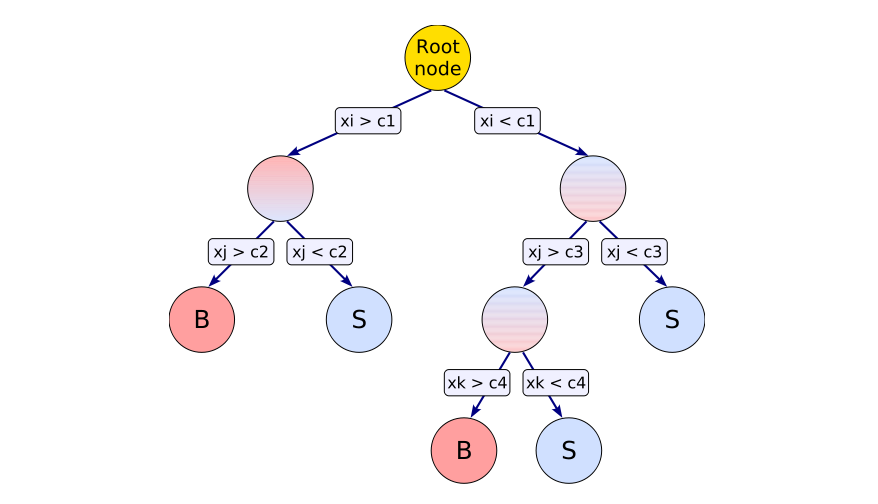
\includegraphics[width=0.7\textwidth]{BDT.png}
\caption{Schematic view of a decision tree. Starting from the \emph{root node}, a sequence  of binary splits using the discriminating variable $x_i$ is applied to the data. The leaf nodes at the bottom end of the tree are labeled ``S'' for signal and ``B'' for background depending on the majority of events that end up in the respective nodes~\cite{Hocker:2007ht}.} % Image taken from Reference~\cite{Hocker:2007ht}.}
\label{fig:BDTsketch}
\end{figure}



\section{The double $b$-hadron jet tagger}

Three variables were selected for training the multivariate methods described in the previous section, based on discrimination power, correlation and pile-up dependence: the jet track multiplicity, the track-jet width and the $\Delta R$ between the axes of two $k_t$ subjets in the jet.  Signal and background datasets were given to the multivariate methods as input, containing a list of the $b$-tagged jets with the information of their $\pt$ and values for the chosen tracking variables.
%Event samples of single and merged $b$-jets, with the information of the value of the selected variables plus their correlations  
 Other variables such as $\tau_2$ or $\max\{\Delta R(trk,trk)\}$ were also tested leading to no gain in performance.


\subsubsection{Selection of an MVA method}

A sub-set of the dijet Monte Carlo sample was used for training the methods in the context of the Toolkit for Multivariate Data Analysis, TMVA \cite{Hocker:2007ht}, written in C++ language.  After the event and jet selections, described in Section~\ref{sec:EventSelection}, were performed, the $b$-tagged jets were classified as signal (single $b$-jets) or background (merged $b$). 

%Based on discrimination power, correlation and pile-up dependence, three variables were selected for the training: the jet track multiplicity, the track-jet width and the $\Delta R$ between the axes of two $k_t$ subjets in the jet.  Signal and background datasets were given to the multivariate methods as input, containing a list of the $b$-tagged jets with the information of their $\pt$ and values for the chosen tracking variables.
%%Event samples of single and merged $b$-jets, with the information of the value of the selected variables plus their correlations  
% Other variables such as $\tau_2$ or $\max\{\Delta R(trk,trk)\}$ were also tested leading to no gain in performance.

%Different training options were evaluated for the likelihood and Neural Network classifiers. 
Two different likelihood configurations were evaluated: the simple likelihood ratio estimator,  using an adaptive Gaussian KDE strategy for the estimation of the PDFs of the input variables; and the more sophisticated PDE-RS approach, adopting an adaptive mode for the volume search.  The multidimentional PDE-RS classifier offered no gain in discrimination with respect to the more simpler likelihood method, with the further disadvange of being more time consuming.  The likelihood method shows good performance, and, given the low correlation of the input variables accross $\pt$, constitutes an adequate method for single-merged discrimination with a fast training step.

An Multi-layer perceptron (MLP) neural net, with two hidden layers of $n_{var}$ and $n_{var}-1$ neurons respectively, was also trained ($n_{var}=3$).  Two different neuron activation functions were tested, $tanh$ and $sigmoid$, with the latter showing better performance.  The initial NN training was carried out in 600 cycles, also termed ``epochs'', for a fast implementation of the method. Although, faster, this configuration led to an irregularly shaped output. This was only fixed with a 3000-epoch training.  

The Boosted Decision Tree (BDT) approach was implemented with 400 trees in the BDT forest. Due to the simplicity of the method where each training step (node splitting) involves only a one-dimensional cut optimisation, little tuning was required in order to obtain reasonably good results.

Examples of the distributions of the final output for these methods, evaluated in an orthogonal sample of simulated dijet events, are displayed in Fig.~\ref{fig:diffmethodsPerfBins} for a medium $\pt$ bin.  %The testing sample satisfies the same selection used for the training sample.
 %When building a network two rules should be kept in mind. The first is the theorem by Weierstrass, which if applied to neural nets, ascertains that for a multilayer perceptron a single hidden layer is  sufficient to approximate a given continuous correlation function to any precision, provided that a sufficiently large number of neurons is used in the hidden layer. If the available computing power and the size of the training data sample suffice, one can increase the number of neurons in the hidden layer until the optimal performance is reached.

The outputs of the explored MVA discriminants are different in terms of shape and range, although the latter could be rearranged with a suitable variable transformation.  In spite of these distinct features the performances of the different methods agree within statistics, see Fig.~\ref{fig:diffmethodsPerfBins}.  
The performance of a classifier algorithm can be assessed by a curve of rejection of merged $b$-jets, ($1/\epsilon_{bkg}$), as a function of single $b$-jet efficiency, $\epsilon_{sig}$; where $\epsilon_{bkg}$ ($\epsilon_{sig}$) is the probability that a double (single) $b$-hadron jet passes the single $b$-jet tagger. The different points in the curve are obtained by varying the likelihood value above which a jet was classified as single (see Section~\ref{sec:btaggingalgos}).

As opposed to NN discriminants with large number of training cycles, the training and the application of the likelihood are very fast operations that are suitable for very large data sets and tuning of the training parameters. Although also very fast, a shortcoming of decision trees is their instability with respect to statistical fluctuations in the training sample from which the tree structure is derived. If two input variables exhibit similar separation power, a fluctuation in the training sample may cause the tree growing algorithm to decide to split on one variable, while the other variable could have been selected without that fluctuation. In such a case the whole tree structure is altered below this node, possibly resulting also in a substantially different classifier response~\cite{Hocker:2007ht}. It is for these reasons that the likelihood classifier is the selected method for our tagger.

\begin{figure}[tp]
\centering
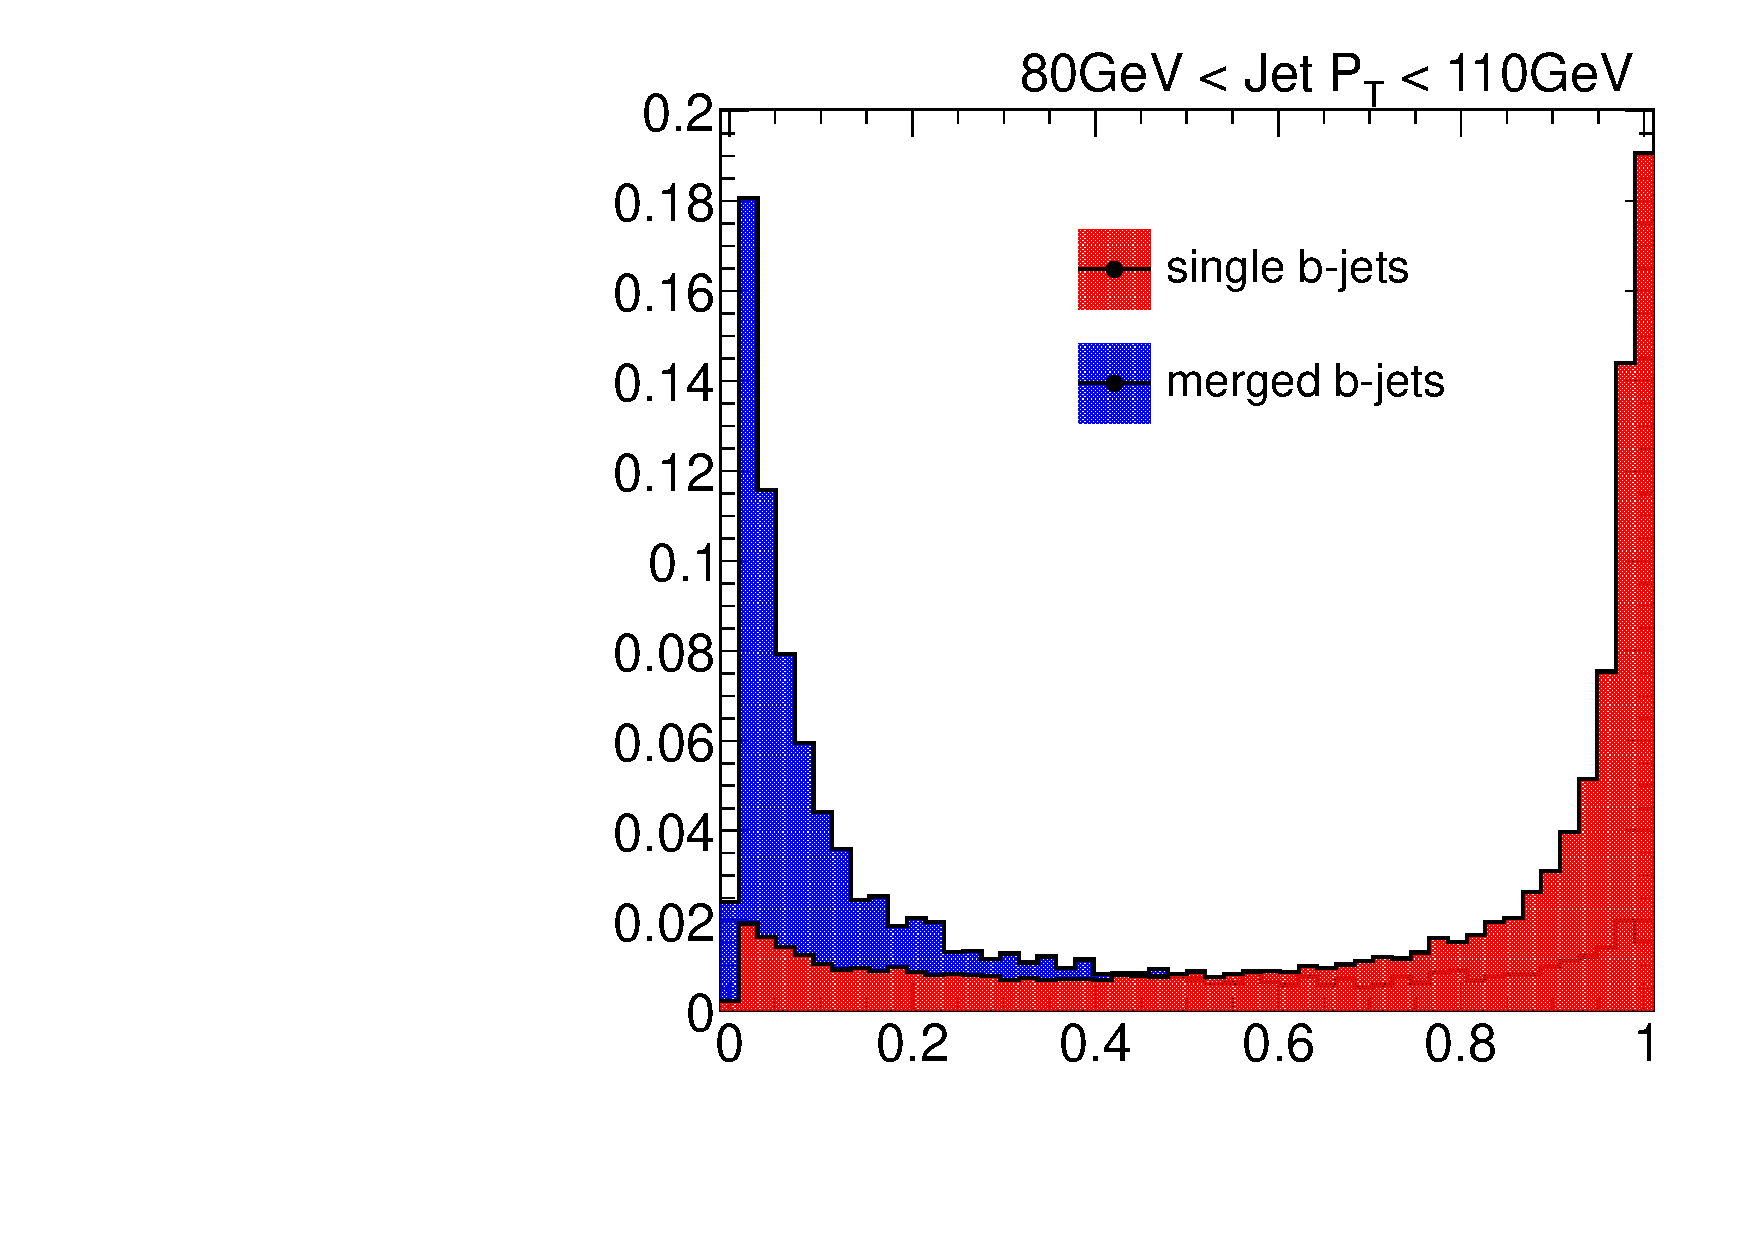
\includegraphics[width=0.32\textwidth]{FIGS/Likelihood/NNoutput080_LihoodKDE.pdf}
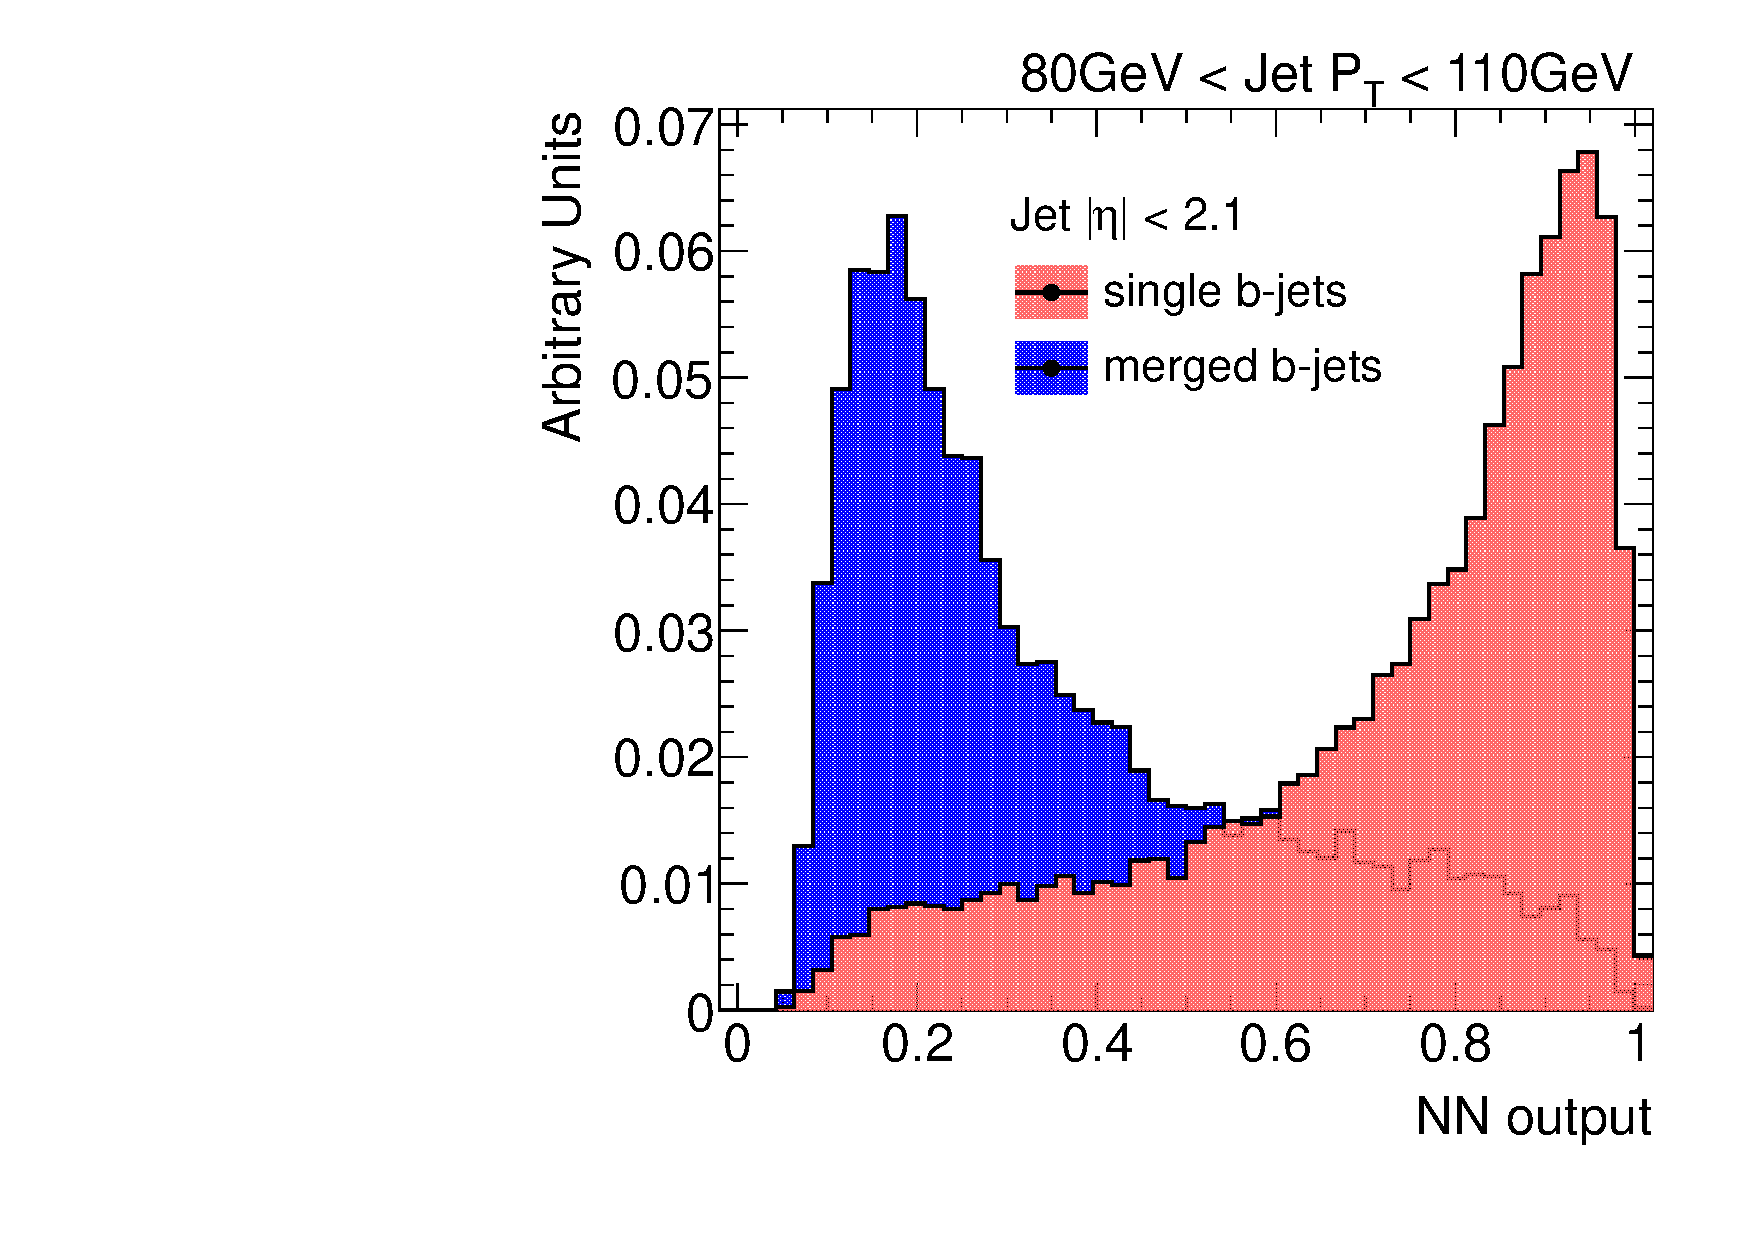
\includegraphics[width=0.32\textwidth]{FIGS/Likelihood/NNoutput080_MLP.pdf}
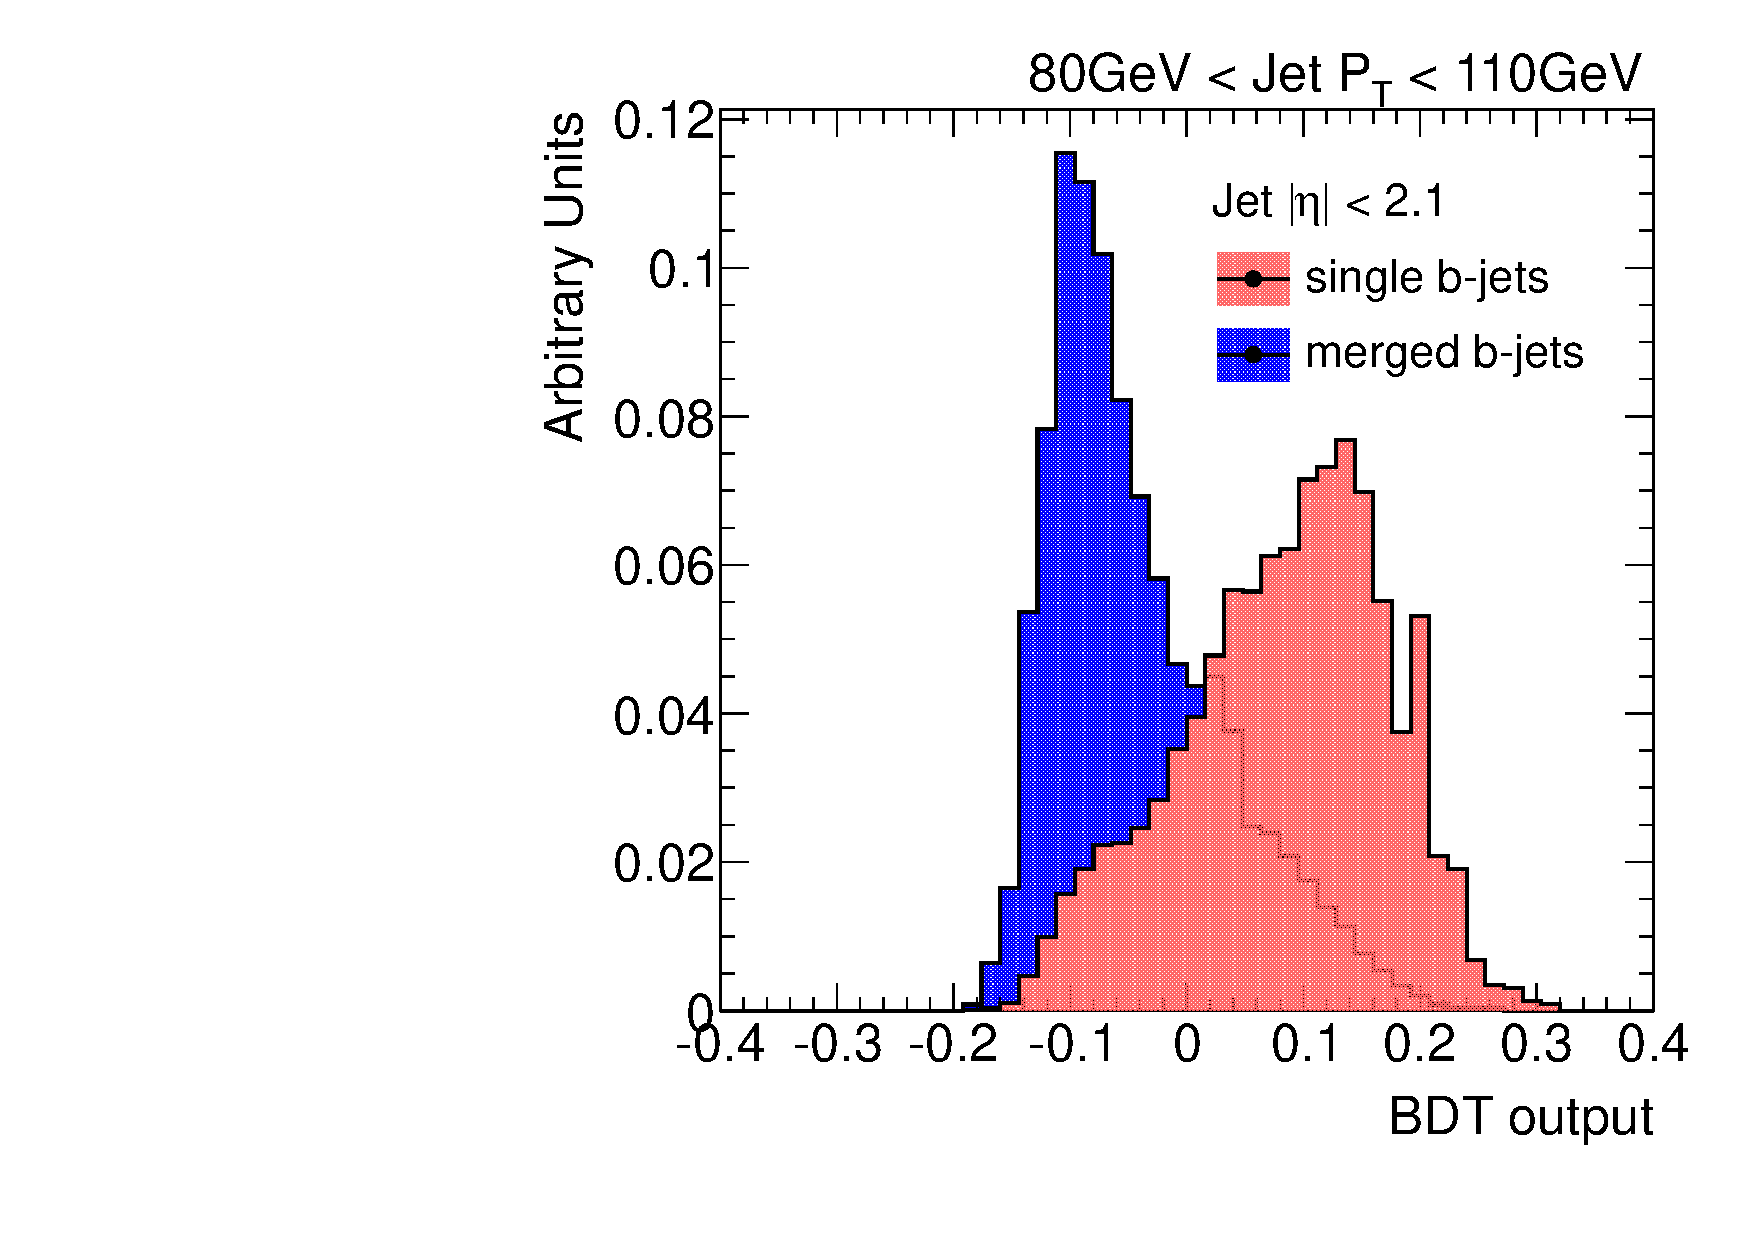
\includegraphics[width=0.32\textwidth]{FIGS/Likelihood/NNoutput080_BDT.pdf}
\caption{Distribution of the MVA discriminant outputs for the Likelihood (a), Neural Network (b) and Boosted Decision Trees (c) classifiers, for single and merged $b$-jets between 80~GeV and 110~GeV.}
\label{fig:diffmethodsBins}
\end{figure}


\begin{figure}[tp]
\centering
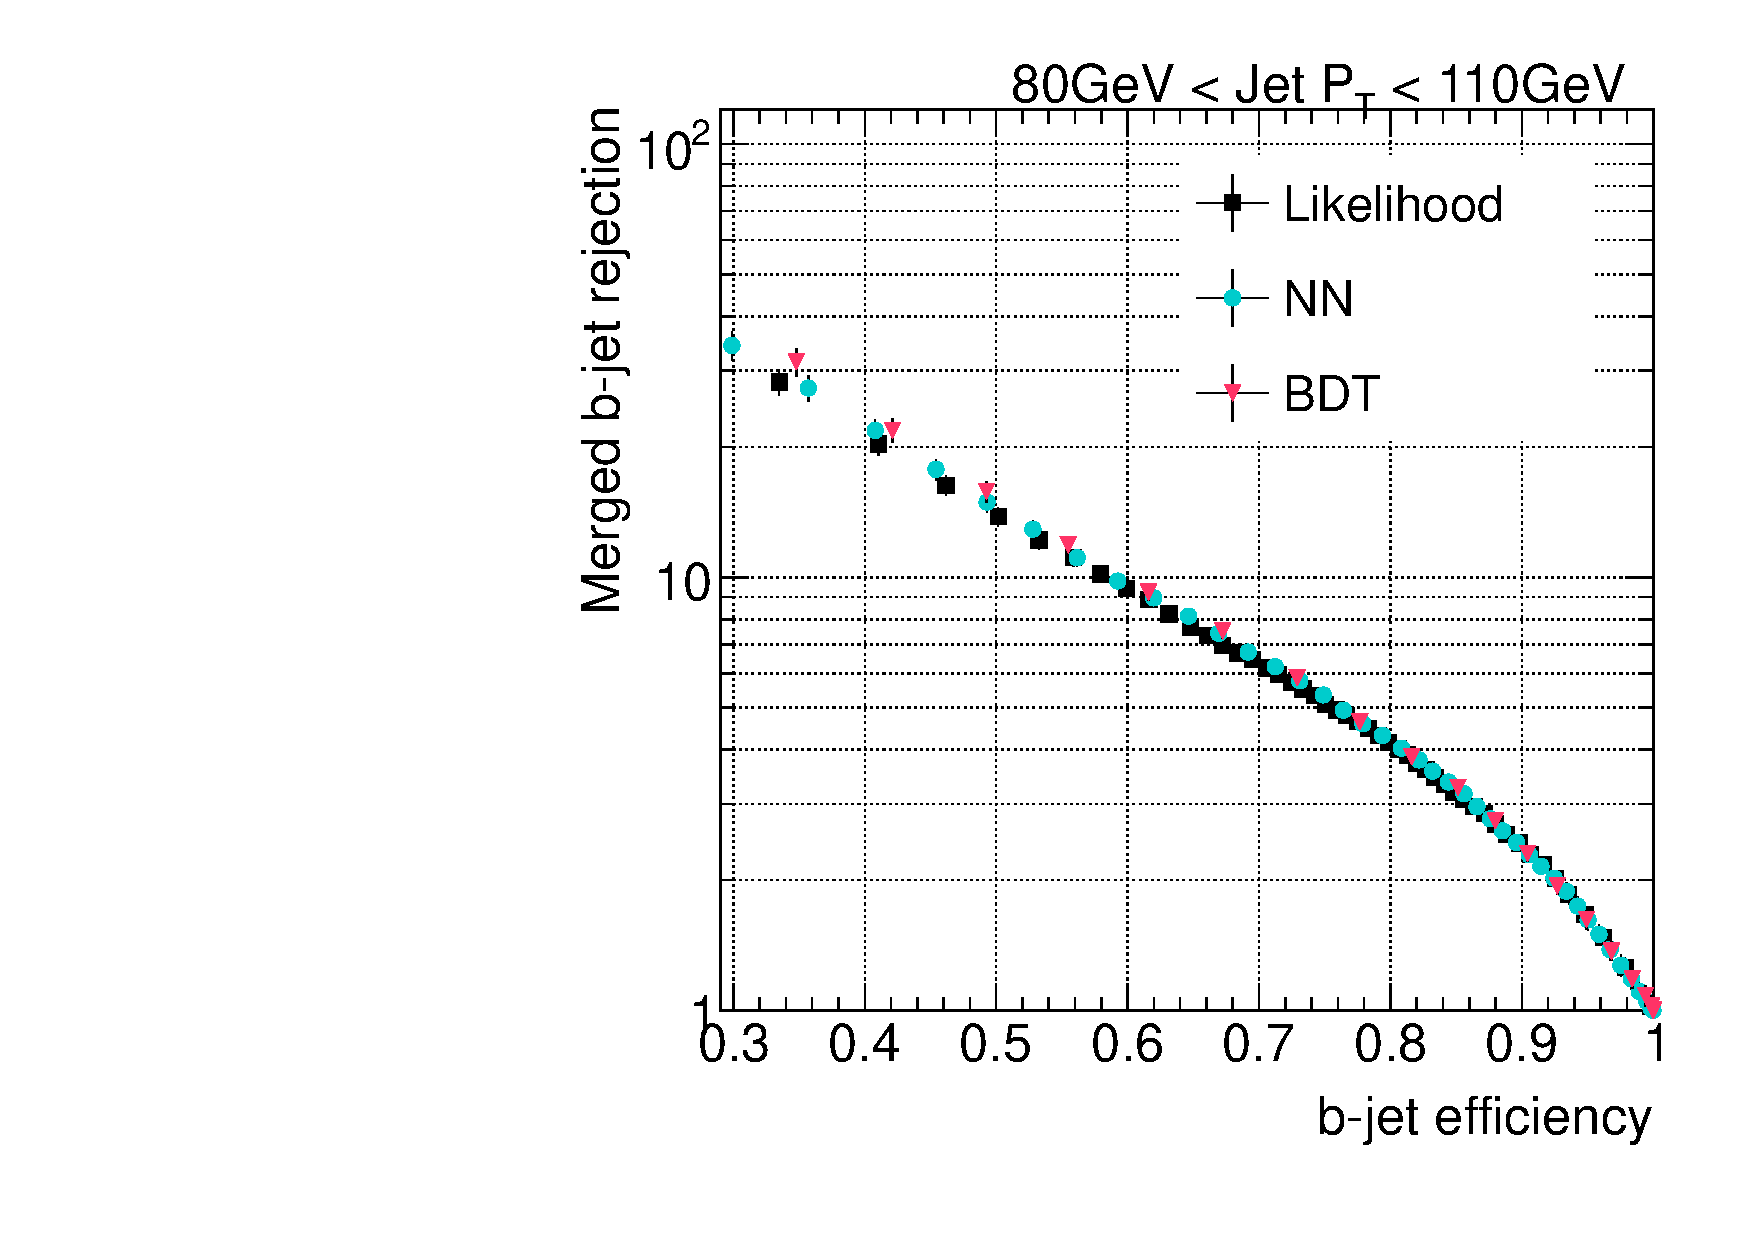
\includegraphics[width=0.49\textwidth]{FIGS/TEMPFigs/MVA_differentMethods/bins/MVAs_RejvsEff80.pdf}
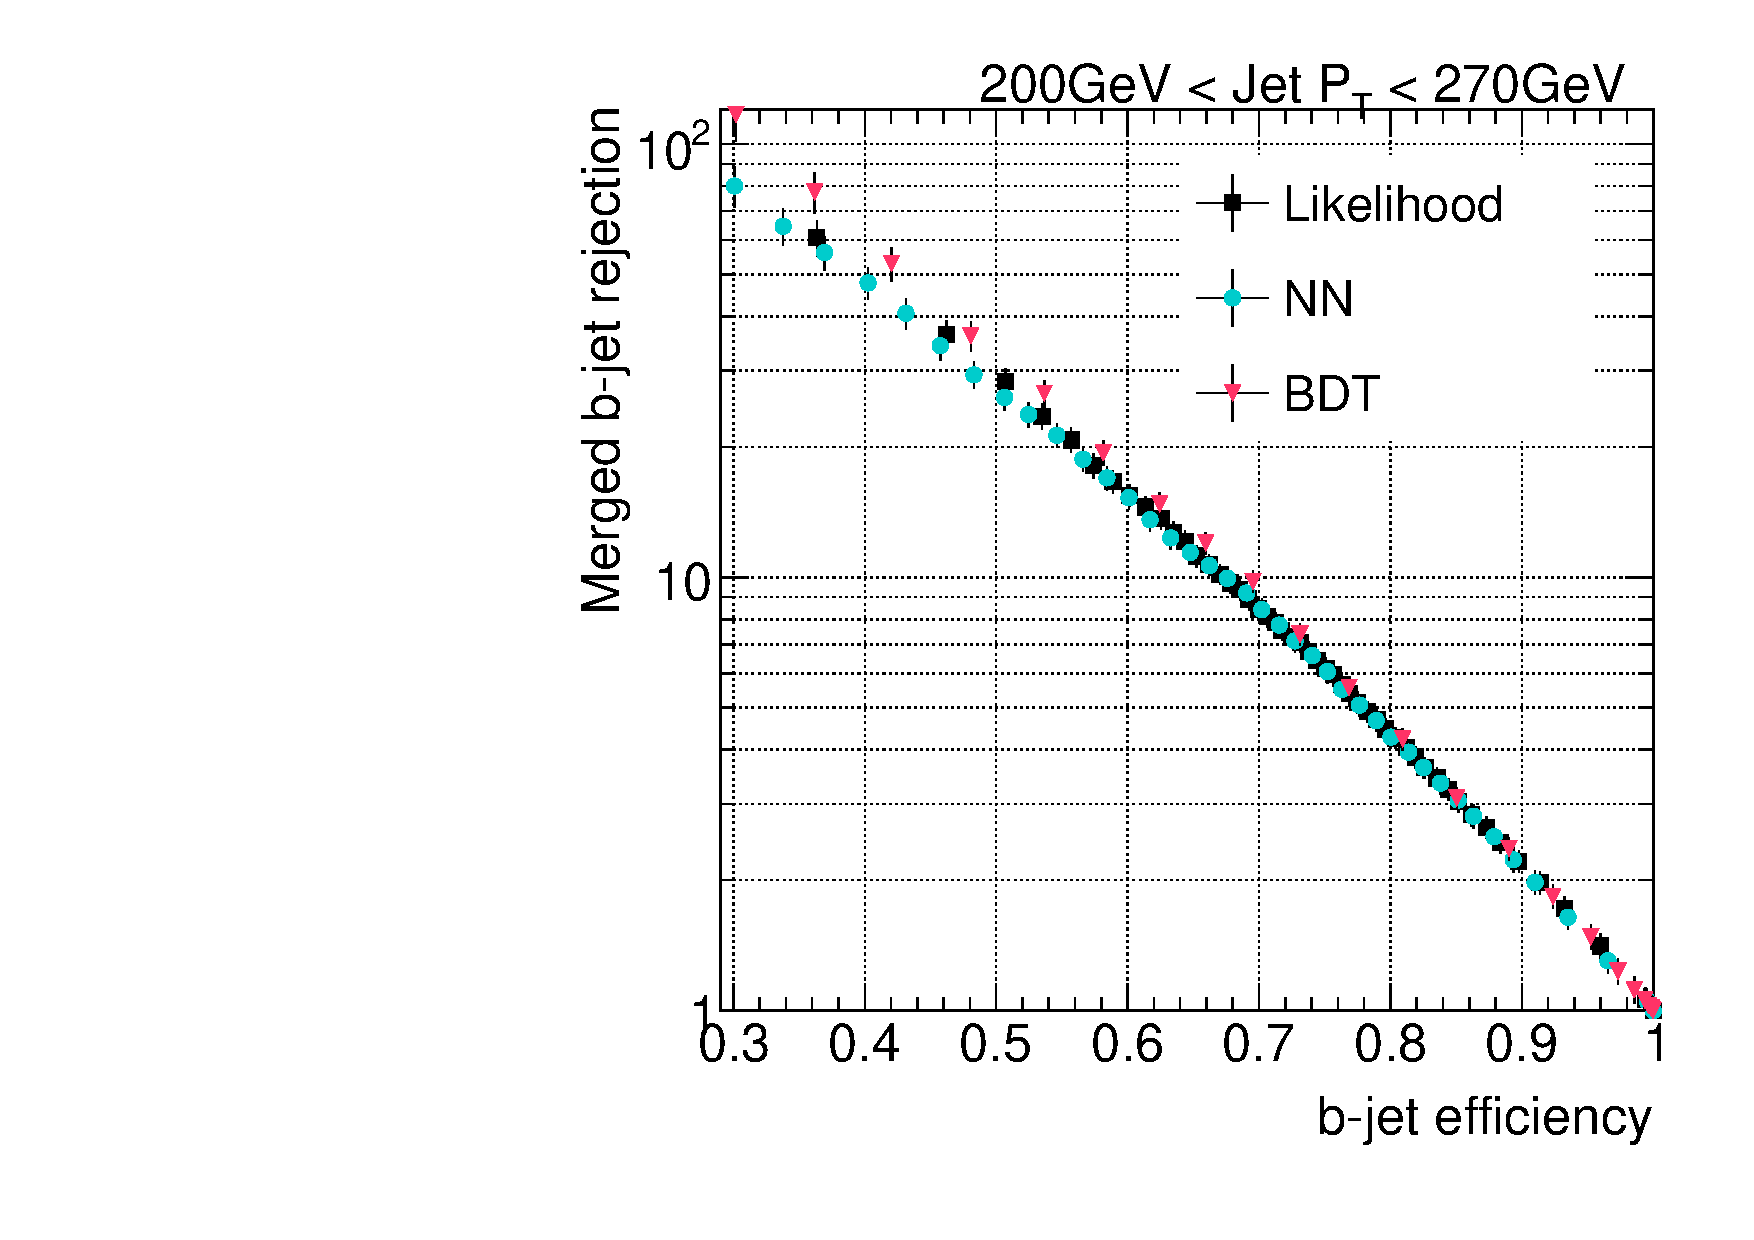
\includegraphics[width=0.49\textwidth]{FIGS/TEMPFigs/MVA_differentMethods/bins/MVAs_RejvsEff200.pdf}
\caption{Rejection of merged $b$-jets as a function of single $b$-jet efficiency for the the different MVA methods evaluated for medium and high jet $\pt$.}
\label{fig:diffmethodsPerfBins}
\end{figure}



%------------------------------------------------------------------------
%\section{$\bm{ g\rightarrow b\bar{b}}$ likelihood training and performance}
%\section{$g\rightarrow b\bar{b}$ likelihood training and performance}
%\section{Likelihood training and performance}
\section{Results obtained}
%------------------------------------------------------------------------

%PEAKS AT 0 - 1
%If a data-mining problem offers a large number of input variables, or variables with excellent separation power, the likelihood response yL is often strongly peaked at 0 (background) and 1 (signal). Such a response is inconvenient for the use in subsequent analysis steps. TMVA therefore allows to transform the likelihood output by an inverse sigmoid function that zooms into the peaks
%yL (i) −→ yL (i) = −τ −1 ln yL − 1 , (37)
%where τ = 15 is used. Note that yL (i) is no longer contained within [0, 1] (see Fig. 11). The transformation (37) is enabled (disabled) with the booking option TransformOutput=True(False).

%The neglect of correlations between input variables in the model, often leads to a diminution of the discrimination performance. Positive correlations lead to peaks at both yL → 0, 1. Correlations can be reduced by categorising the data samples and building an independent likelihood classifier for each event category. Such categories could be geometrical regions in the detector, kinematic properties, etc.



A discriminant between single and merged $b$-jets was built by training a likelihood ratio estimator, with the following three variables as input, 
%
\begin{enumerate}\addtolength{\itemsep}{-0.4\baselineskip}
\item
Jet track multiplicity
\item
Track-jet width
\item
$\Delta R$ between the axes of 2 $k_t$ subjets within the jet
\end{enumerate}
%

Given the correlation of the variables with the jet transverse momentum,  the training sample was categorized in bins of calorimeter jet $\pt$, and independent likelihood classifiers were built for each category.  

Due to the lack of statistics 
%In order to increase the statistics 
of merged jets in the low $\pt$ bins, signal and background jets were not weighted by the dijet samples cross-sections to allow the contribution of subleading lower $\pt$ jets from high $\pt$ events. The gain in statistics in merged $b$-jets for the first $\pt$ bin was of more than 500\%.   It is important to stress that, although essential for data to MC comparisons (see Section~\ref{sec:analysis}), the weighting of the dijet Monte Carlo samples by their respective cross-sections is not necessary for studies performed at simulation level only.
For the evaluation of the method the same procedure was followed.

Example distributions of the likelihood output for single and merged $b$-jets are displayed in  Fig.~\ref{fig:outputinbins} for low and high transverse momentum jets.  The performance plot including the rejection vs. efficiency curves for each of the eight $\pt$ bins studied (see Section~\ref{sec:EventSelection}) is shown in Fig.~\ref{fig:performanceinbins}. The performance of the tagger improves with $\pt$:


\begin{itemize}\addtolength{\itemsep}{-0.4\baselineskip}
\item
$\pt>40$ GeV: %\\[1mm]
rejection above 8 at 50\% eff.
% over 85\% rejection at 50\% eff.
\item
$\pt>60$ GeV: %\\[1mm]
rejection above 10 at 50\% eff.
 %90\% rejection at 50\% eff.
\item
$\pt>200$ GeV: %\\[1mm]
rejection above 30 at 50\% eff.
 %over 95\% rejection at 50\% eff.
\end{itemize}


\begin{figure}[tp]
\centering
%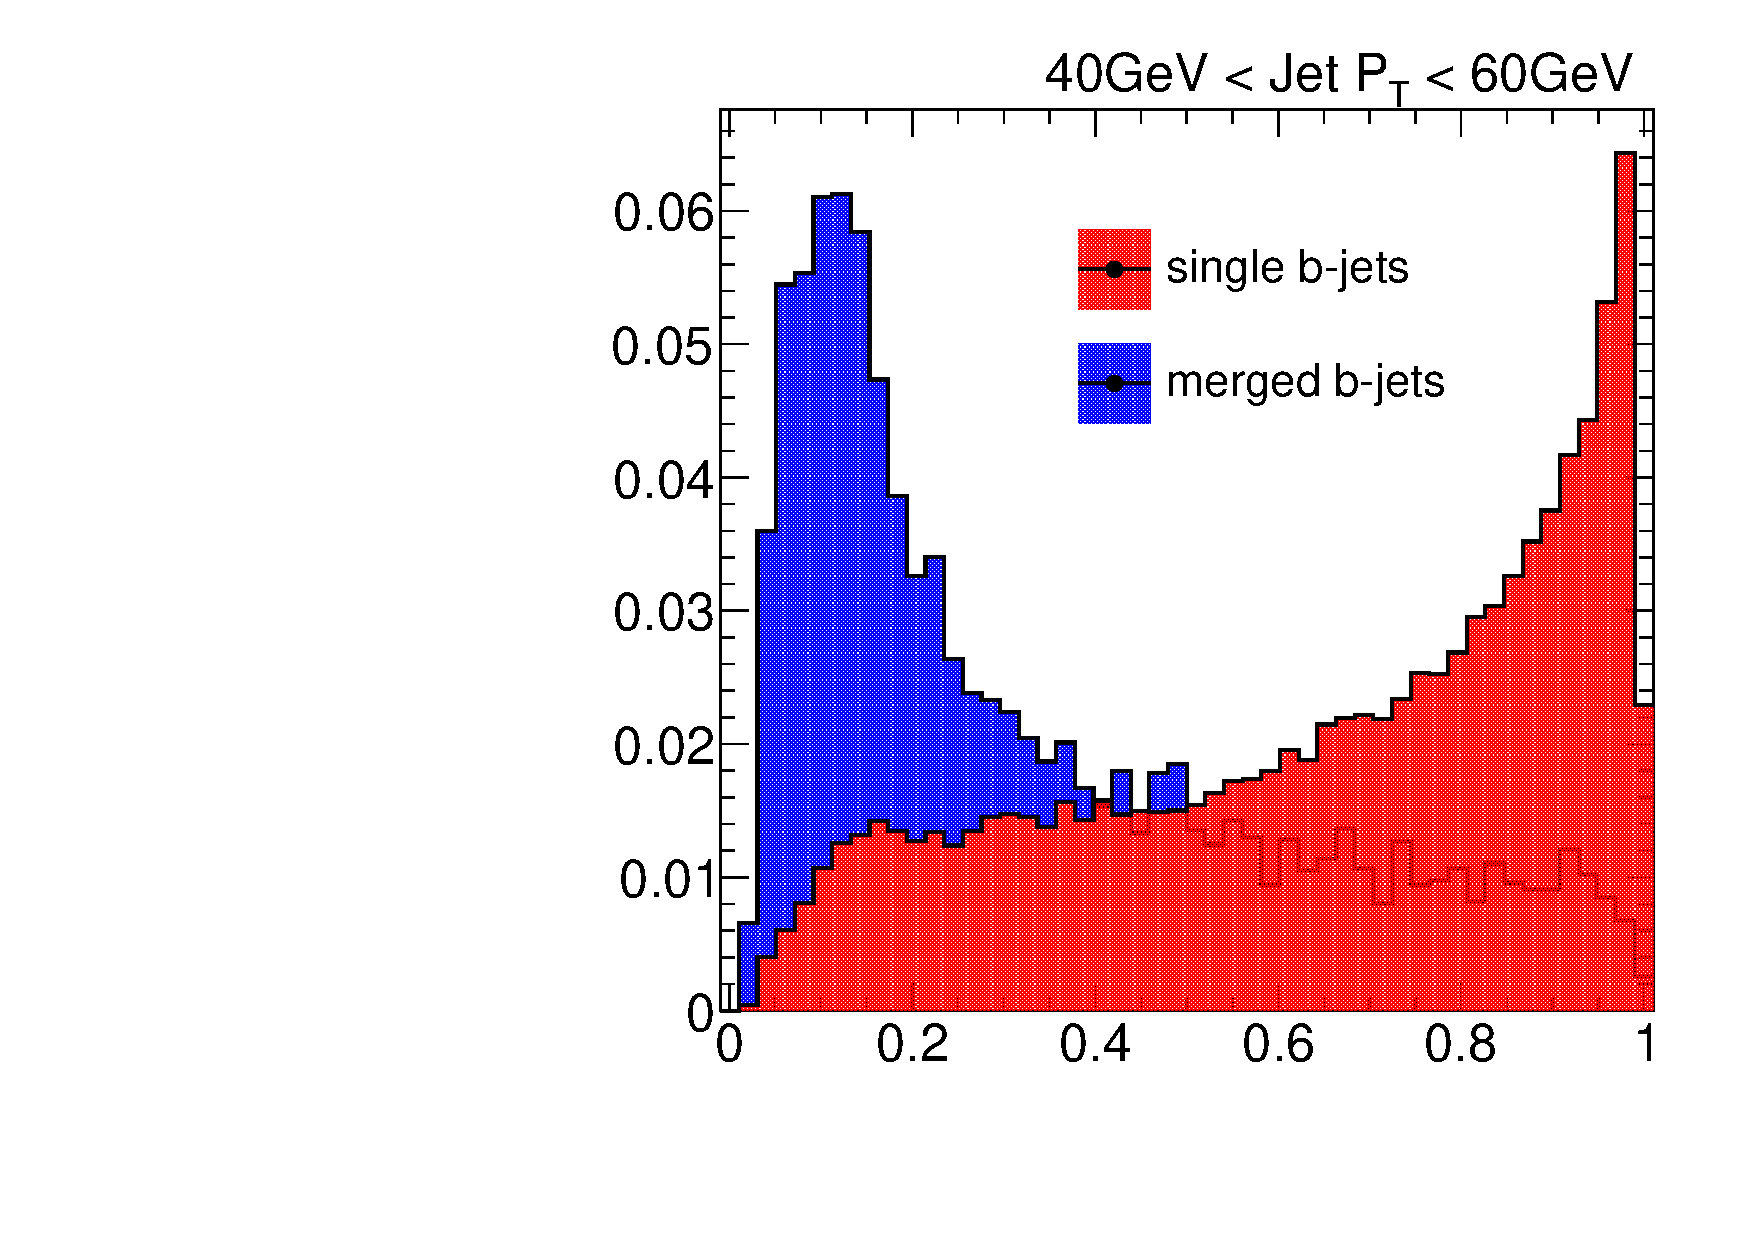
\includegraphics[width=0.32\textwidth,viewport=40 0 540 550]{FIGS/Likelihood/NNoutput040_LihoodKDE.pdf}
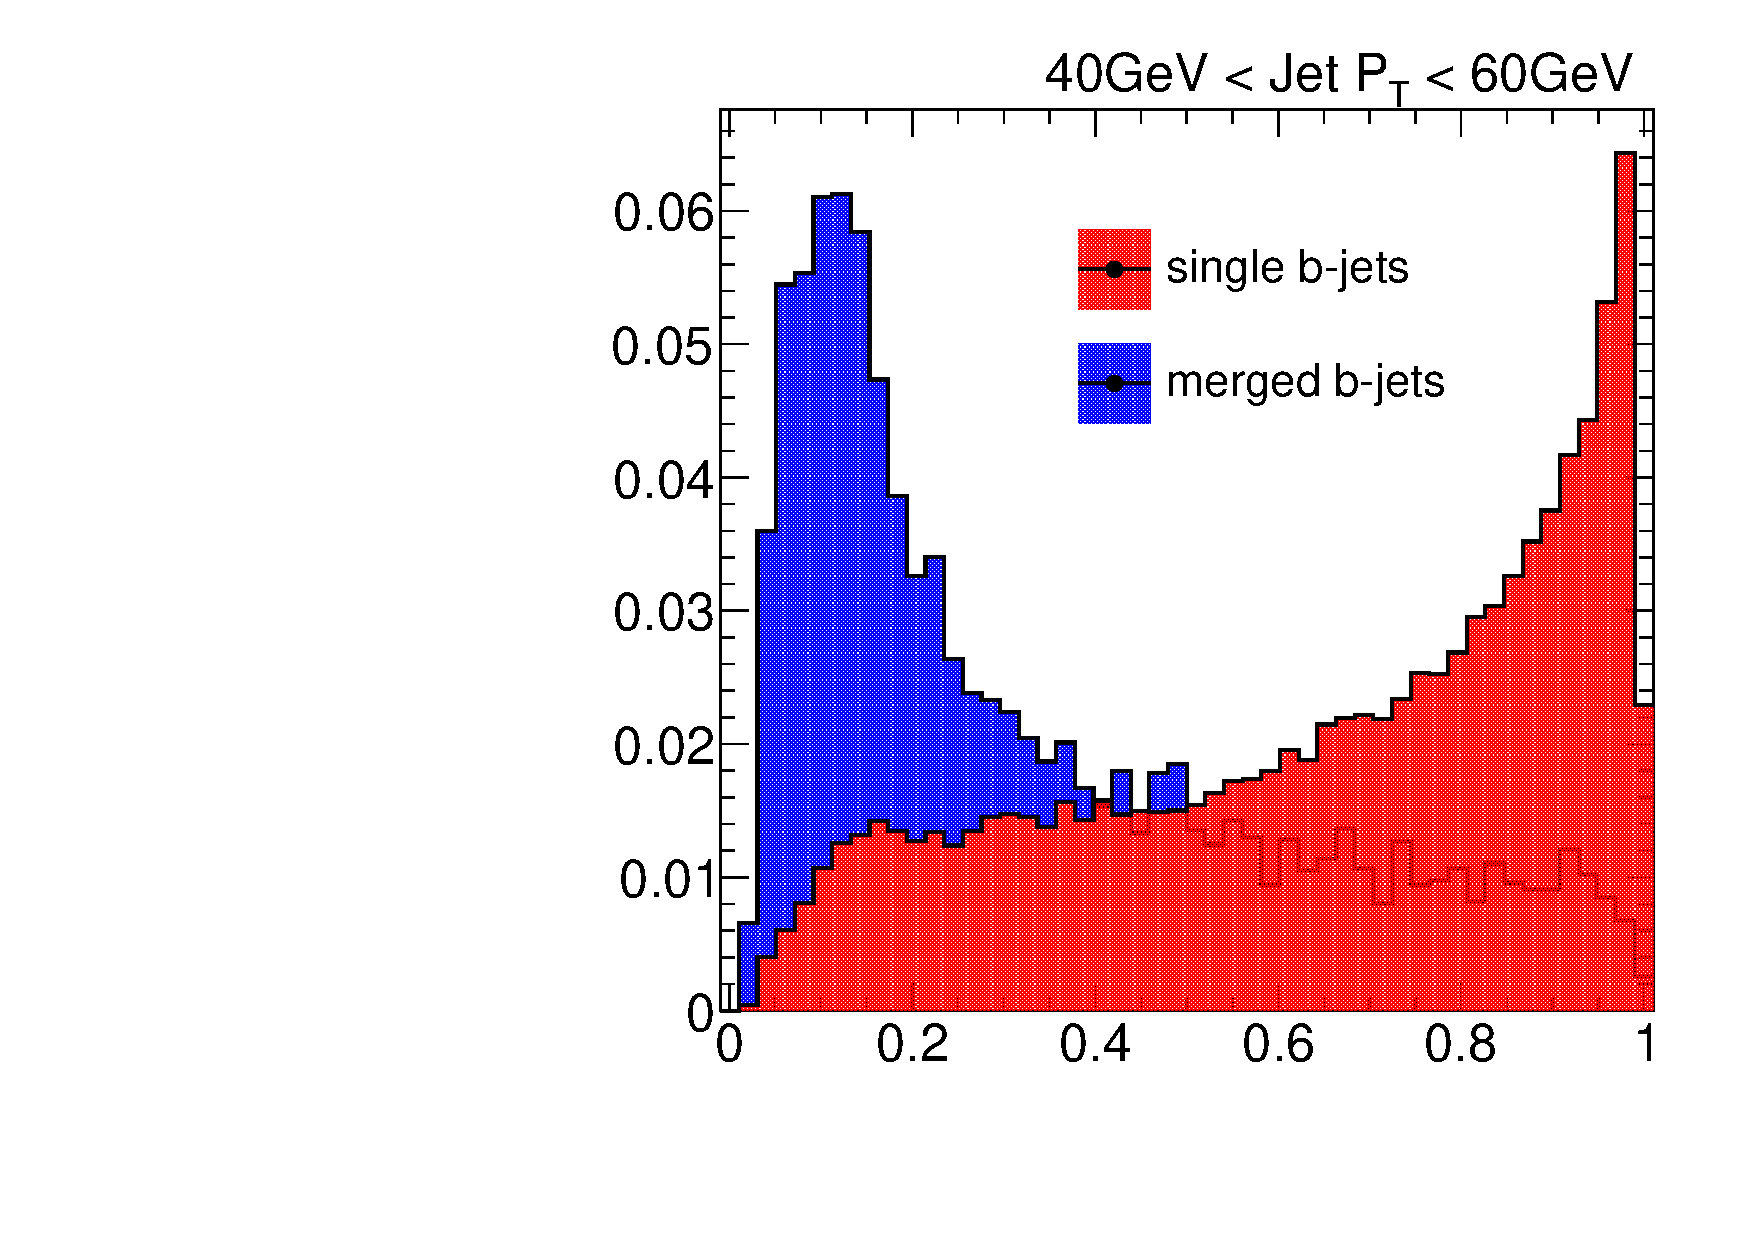
\includegraphics[width=0.49\textwidth]{FIGS/Likelihood/NNoutput040_LihoodKDE.pdf}
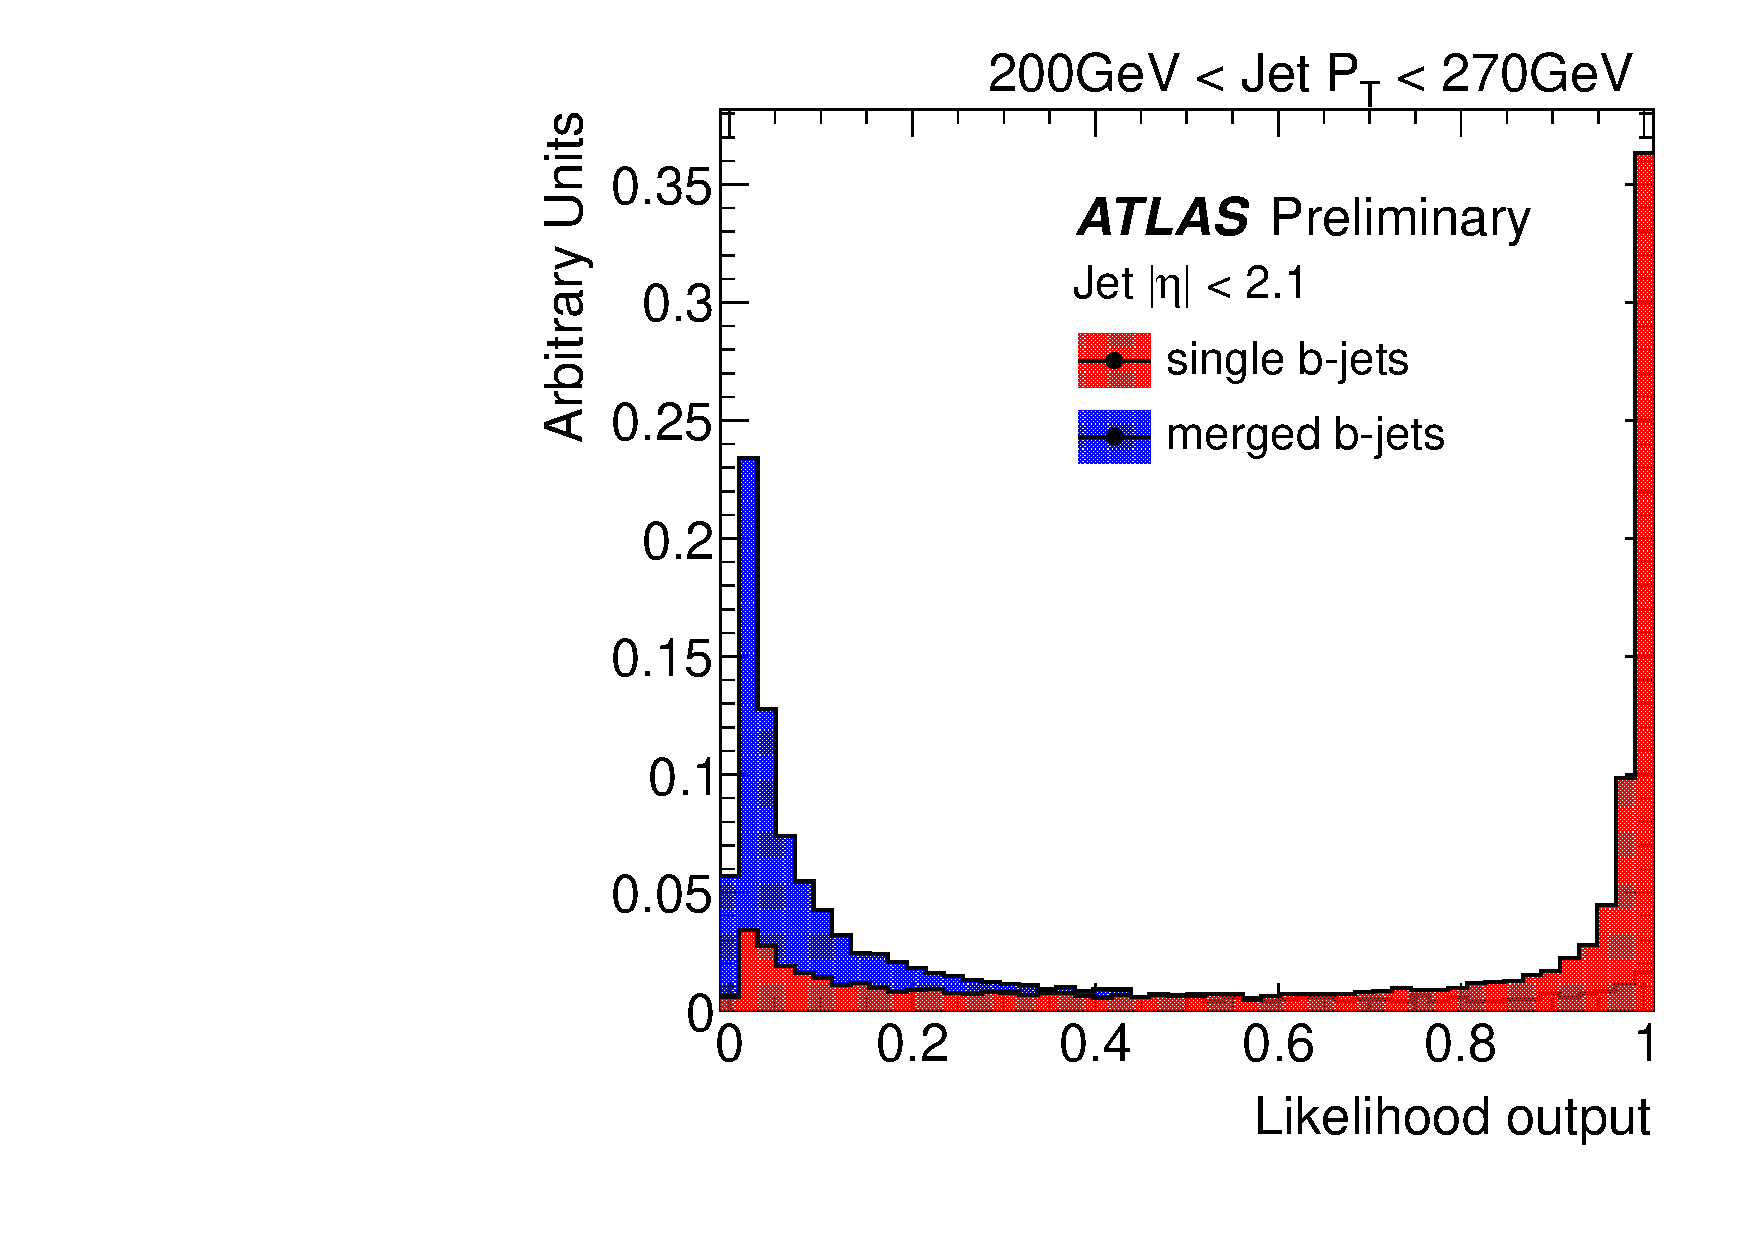
\includegraphics[width=0.49\textwidth]{FIGS/Likelihood/NNoutput200_LihoodKDE.pdf}  
\caption{Distribution of the likelihood output for single and merged $b$-jets for low and high $\pt$ jets.}
\label{fig:outputinbins}
\end{figure}

\begin{figure}[tp]
\centering
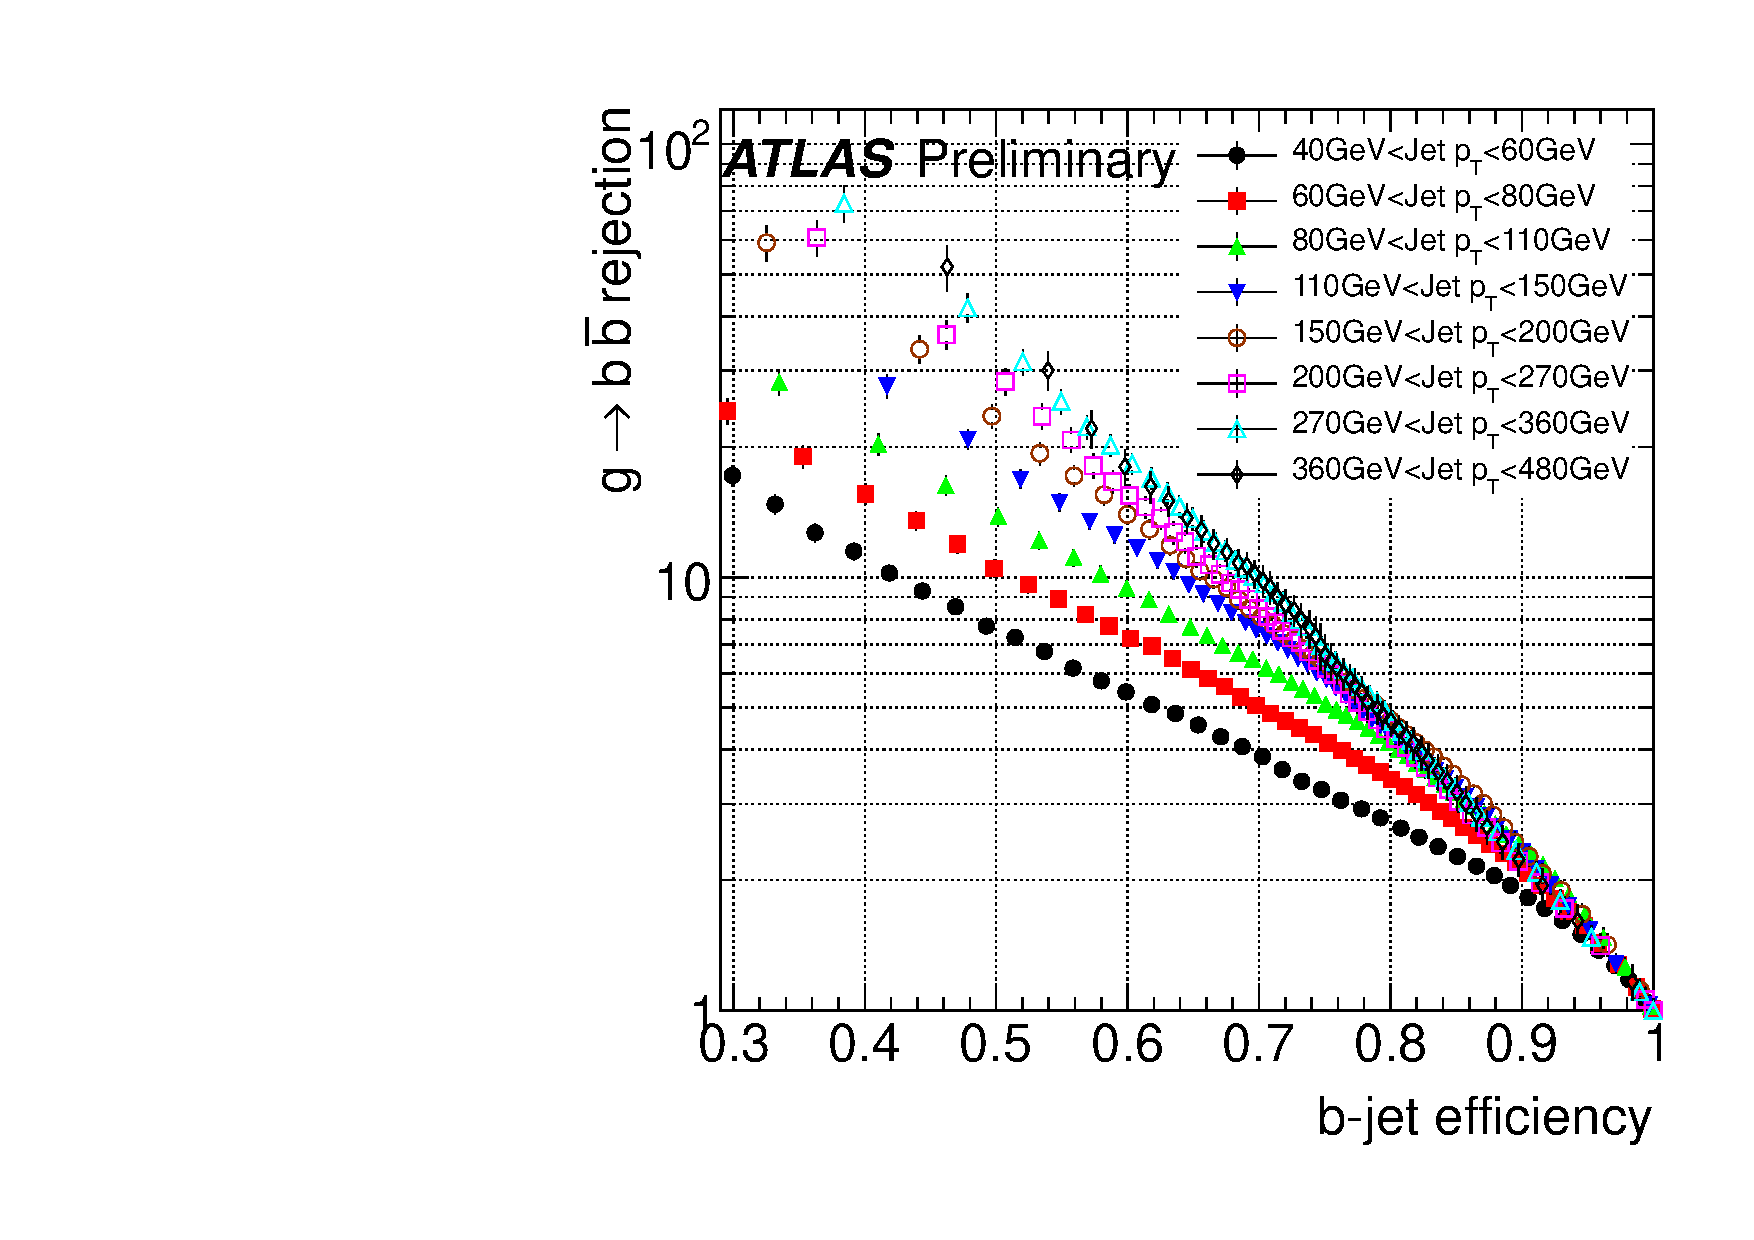
\includegraphics[width=0.7\textwidth]{FIGS/Likelihood/KDE_RejvsEff.pdf}
\caption{Rejection of merged $b$-jets as a function of single $b$-jet efficiency for dijet events in 8 jet $\pt$ bins.}
\label{fig:performanceinbins}
\end{figure}


The rejection of merged jets attained as a function of $\pt$ for the 50\% and 60\% single $b$-jet efficiency working points are summarized in Table~\ref{tb:rejection}, together with their relative statistical error. These are propagated from the Poisson fluctuations of the number of events in the merged and single $b$ distributions. The error is slightly lower for the 60\% efficiency working point because a higher efficiency allows for a greater number of Monte Carlo events to measure the performance. %the higher the efficiency, the larger the number of Monte Carlo events available to measure the performance.




\begin{table}[!hbt] %[h]
\renewcommand{\arraystretch}{1.2}
\centering
\begin{tabular}{ | c || c | c || c | c||}
  \hline
  Jet $\pt$ & \multicolumn{2}{c||}{single $b$-jet efficiency 50\%} & 
            \multicolumn{2}{c||}{single $b$-jet efficiency 60\%}\\ \cline{2-5}
    (GeV )  & ~~Rejection~ & stat.err. & ~~Rejection~ & stat.err. \\ \hline
   40 - 60 &  ~8 &  4\%  &  ~5  &  3\%    \\ 
   60 - 80 &  ~10 &  4\%  &  ~7  &  4\%    \\ 
   80 - 110&  ~14 &  5\%  &  ~9  &  4\%    \\ 
  110 - 150&  19 &  5\%  &  12  &  4\%    \\ 
  150 - 200&  23 &  5\%  &  14  &  5\%    \\ 
  200 - 270&  30 &  7\%  &  16  &  6\%    \\ 
  270 - 360&  36 &  7\%  &  19  &  6\%    \\ 
  360 - 480&  41 &  8\%  &  18  &  8\%    \\ \hline
\end{tabular}
\caption{The merged $b$-jet rejection for the 50\% and 60\% efficiency working points in bins of $\pt$.}
\label{tb:rejection}
\end{table}





%------------------------------------------------------------------------
\section{Systematic uncertainties}\label{sec:gbbSystematics}
%------------------------------------------------------------------------
The development, training and performance determination of the tagger is based on simulated events. Although the agreement between simulation and data explored in section~\ref{sec:gbbValidation} is a necessary validation condition, it is also important to investigate how the tagger performance depends % on systematics relevant in the data. In particular we have considered:
 on the systematic precision with which the MC simulates the data. In particular we have considered:
%
%There are uncertainties in the data that, although not spoiling the data/MC agreement, might change the performance of the tagger. This uncertainties would also be present in an eventual future data-driven determination of the performance as  the data are not known better that this.The following systematic effects have been studied and their influence on the tagger performance ascertained:
%
%In order to study the systematic uncertainties in the method the following contributions were evaluated:
\begin{itemize}\addtolength{\itemsep}{-0.4\baselineskip}
\item
presence of additional interactions (pile-up);
\item
uncertainty in the $b$-jet tagging efficiency; % and b-jet energy scale?
\item
uncertainty in the track reconstruction efficiency;
\item
uncertainty in the track transverse momentum resolution;
\item
uncertainty in the jet transverse momentum resolution;
\item
uncertainty in the jet energy scale.
%the effect of jet isolation
%\item
%other $\Delta R$ cuts for B-labeling and matching
\end{itemize}

{ \em I. Pile-up}
\\[3mm]
  The size of this effect was studied by comparing the performance of the likelihood discriminant with $b$-jets in events with small (1-9) and large (9-20) number of primary vertices. 
A comparison of the performance in these two sub-samples relative to the inclusive sample is shown in Fig.~\ref{fig:performanceinbinsMu} for the two lowest $\pt$ bins, where the effect of pile-up is more important.
As expected from the use of tracking (as opposed to calorimeter) variables, no significant dependence with pile-up is observed. % within statistics. %Of the 16 determinations (2 working points with 8 $\pt$ bins each) of performance differences between high and low number of primary vertices events, it is observed that 6 of them are positive and 10 negative, with a global mean of 0.3\%. We conclude that the effect is negligible compared to other source of uncertainties.
Performance differences between high and low number of primary vertices events are $\leq$~2\%. % and therefore negligible compared to other sources of uncertainties. 
The impact of pile-up might be larger in 2012 data.

%See Fig.~\ref{fig:performanceinbinsMu}.
\begin{figure}[tp]
\centering
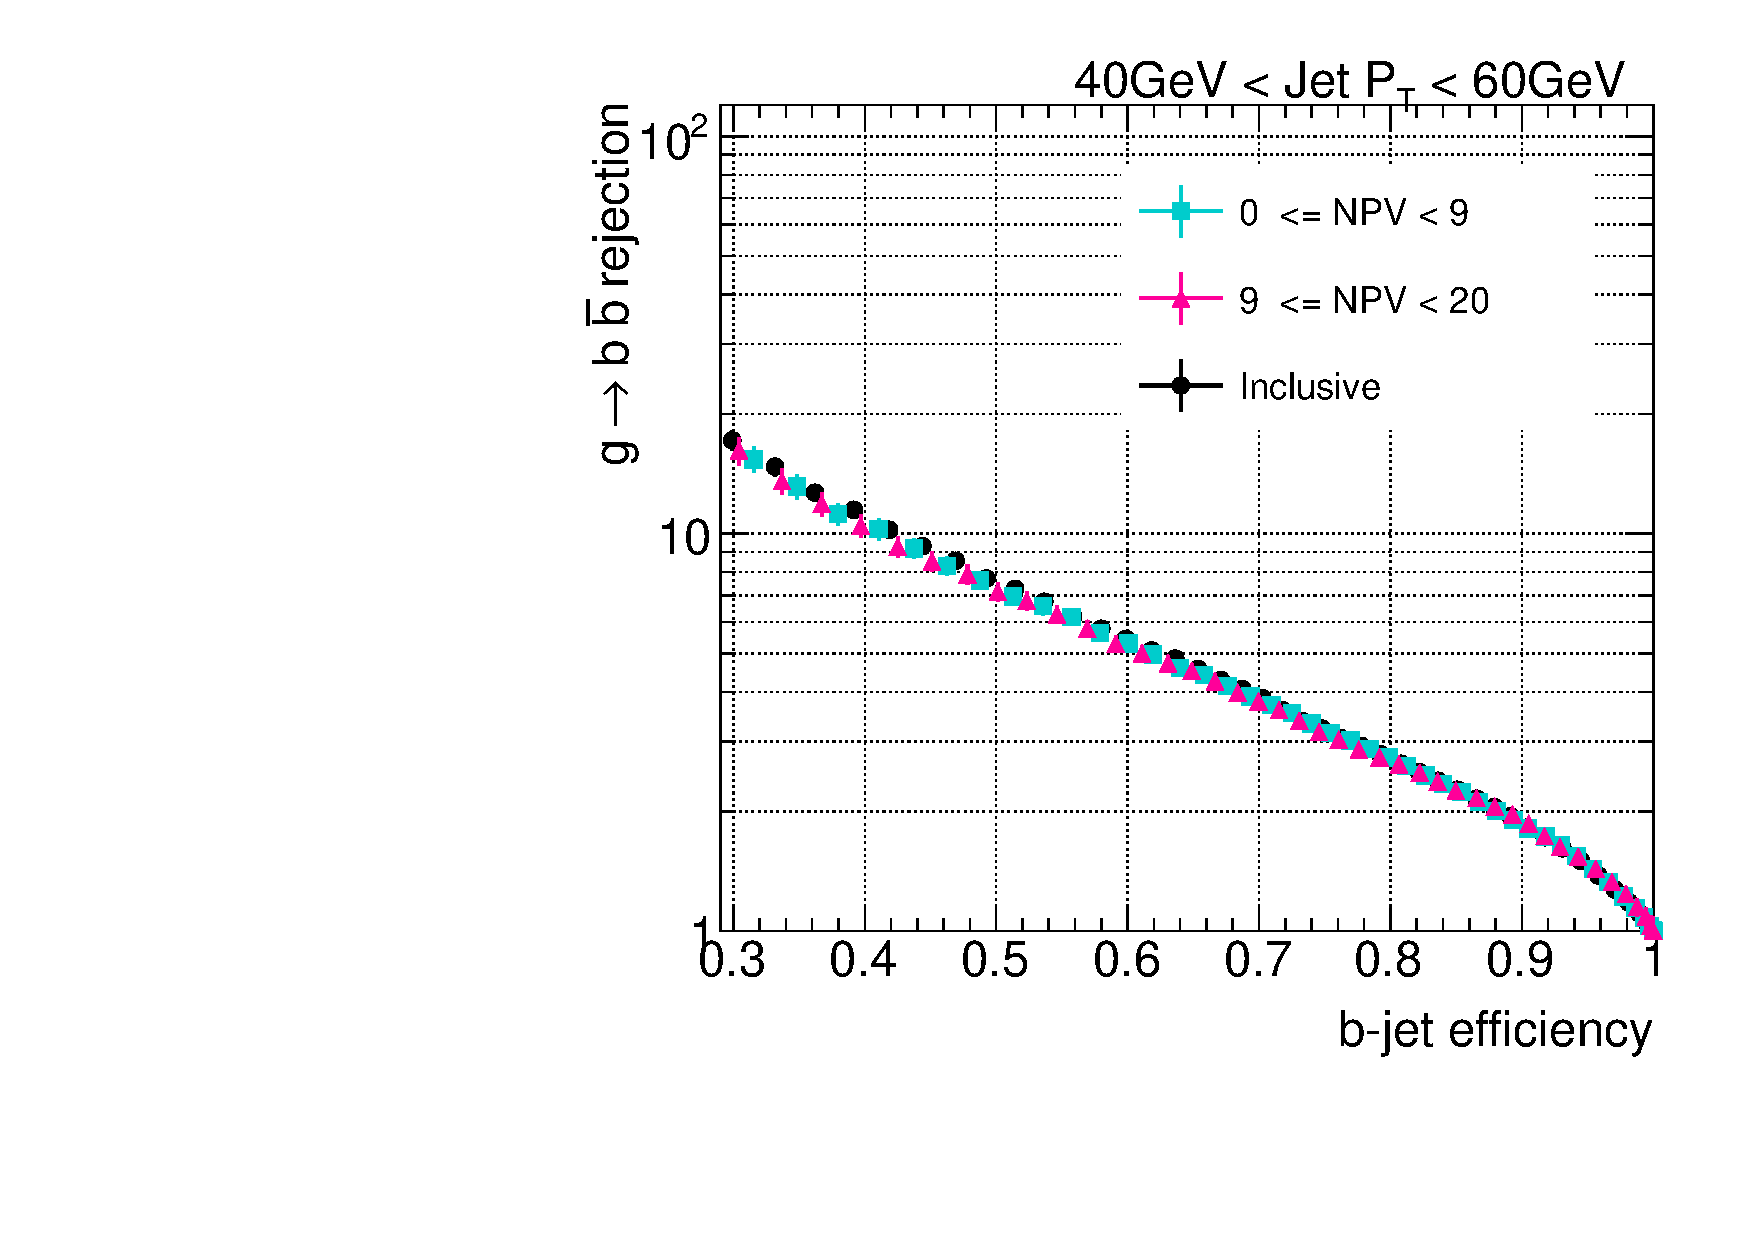
\includegraphics[width=0.49\textwidth]{FIGS/systematics/LlhoodKDE_ISO_PileUp_rejvseff040.pdf}
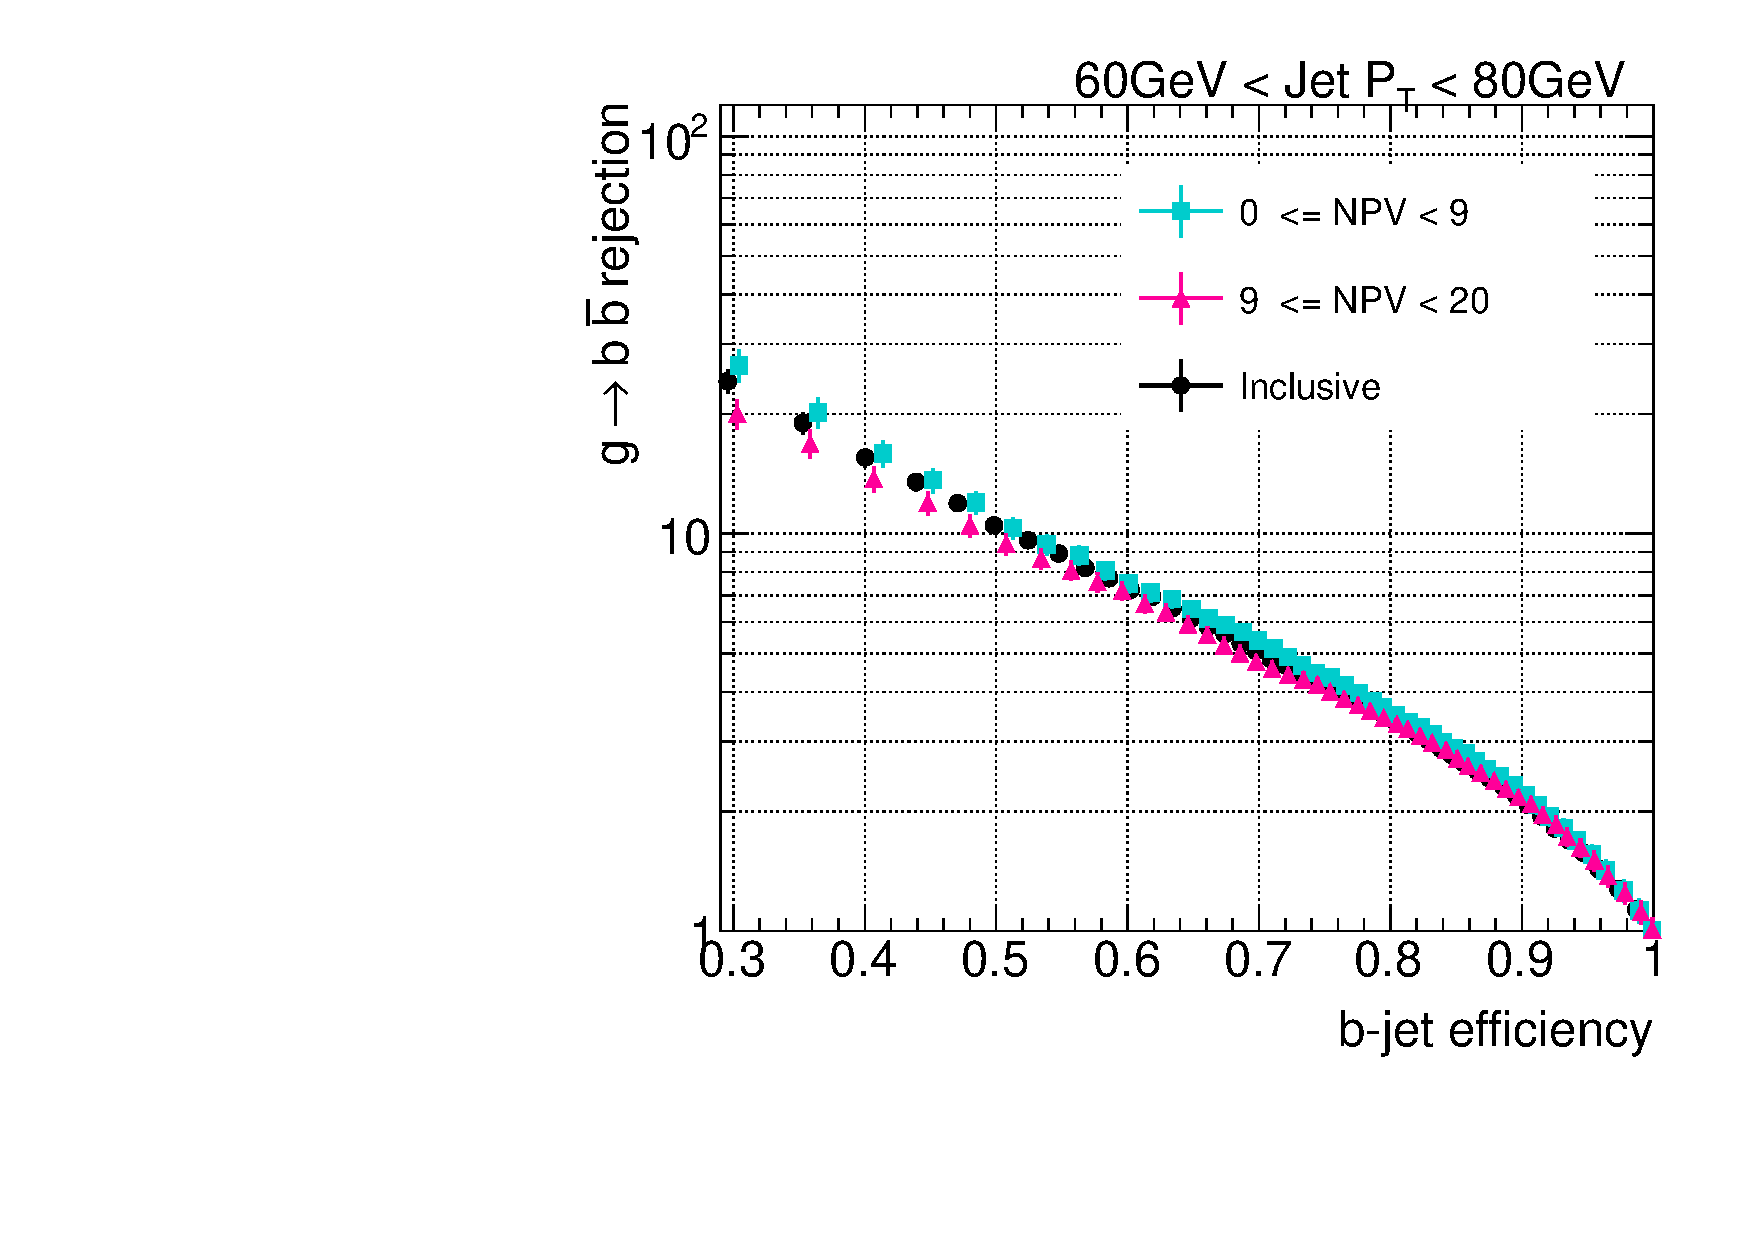
\includegraphics[width=0.49\textwidth]{FIGS/systematics/LlhoodKDE_ISO_PileUp_rejvseff060.pdf}
\caption{Rejection of merged $b$-jets as a function of single $b$-jet efficiency in bins of NPV for two low jet $\pt$ bins.}
\label{fig:performanceinbinsMu}
\end{figure}

\vspace{3mm}
{\em II. b-tagging efficiency} %energy scale and 
\\[3mm]
The performance of heavy-flavor tagging in Monte Carlo events is calibrated to experimental data by means of scale factors (SFs). % measured by the ATLAS Flavour Tagging Working group. 
The SFs are defined as the ratio of the heavy-flavor tagging efficiency in data over that in Monte Carlo for the different jet flavors. They are measured by the ATLAS Flavour Tagging Working group,  %, and probably also as a function of jet pT and η 
%Such a measurement carries a systematic uncertainty, and in order to estimate its effect a conservative approach is followed: %https://twiki.cern.ch/twiki/bin/viewauth/AtlasProtected/BTaggingCalibrationDataInterface
and their measurement carries a systematic uncertainty, see Section~\ref{sec:btagcalib}.  

To estimate the impact of this uncertainty a conservative approach is followed: the SFs are varied in all the $\pt$ bins simultaneously by one standard deviation both in the up and down directions. The MC distributions weighted by the varied SFs show no major deviations from the nominal, see Fig.~\ref{fig:btaggingSFs}.  %The result of this procedure for the distribution of two of the tracking variables used in our discriminant is illustrated in Fig.~\ref{fig:btaggingSFs}. 
In the same manner, the effect of the $b$-tagging calibration uncertainty on the likelihood peformance, shown in Fig.~\ref{fig:btaggingSFsPerf}, is $< 1$\%, negligible with respect to the statistical uncertainty.
% as it can be seen in Fig.~\ref{fig:btaggingSFsPerf}.
This was indeed expected. The scale factors depend on the true flavor of the jet and on its $\pt$, but these are basically constant in the performance determination, which is based on single flavor (true $b$-) jets classified in $\pt$-bins.


\begin{figure}[tp]
\centering
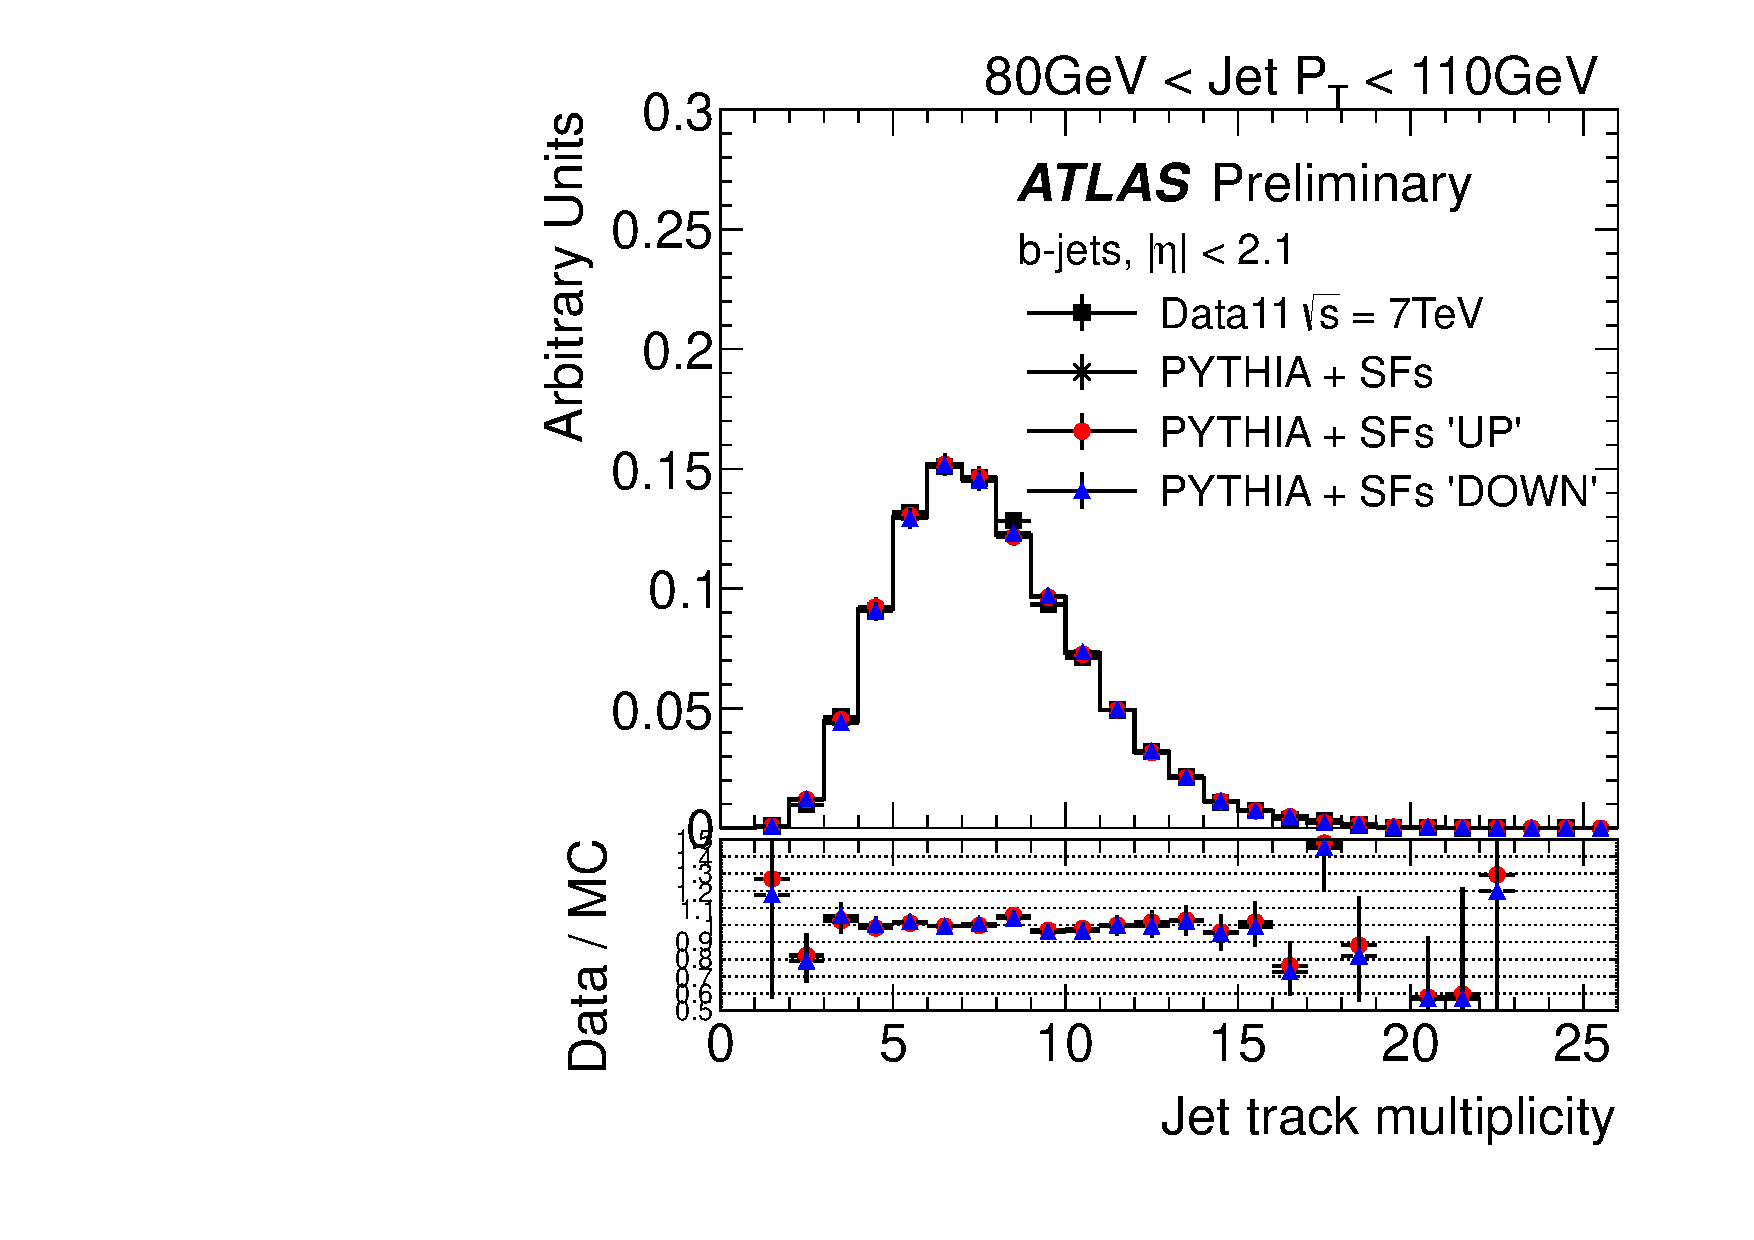
\includegraphics[width=0.49\textwidth]{FIGS/systematics/BTagCalib_DataVarNtrkPT080.pdf}
%%%%%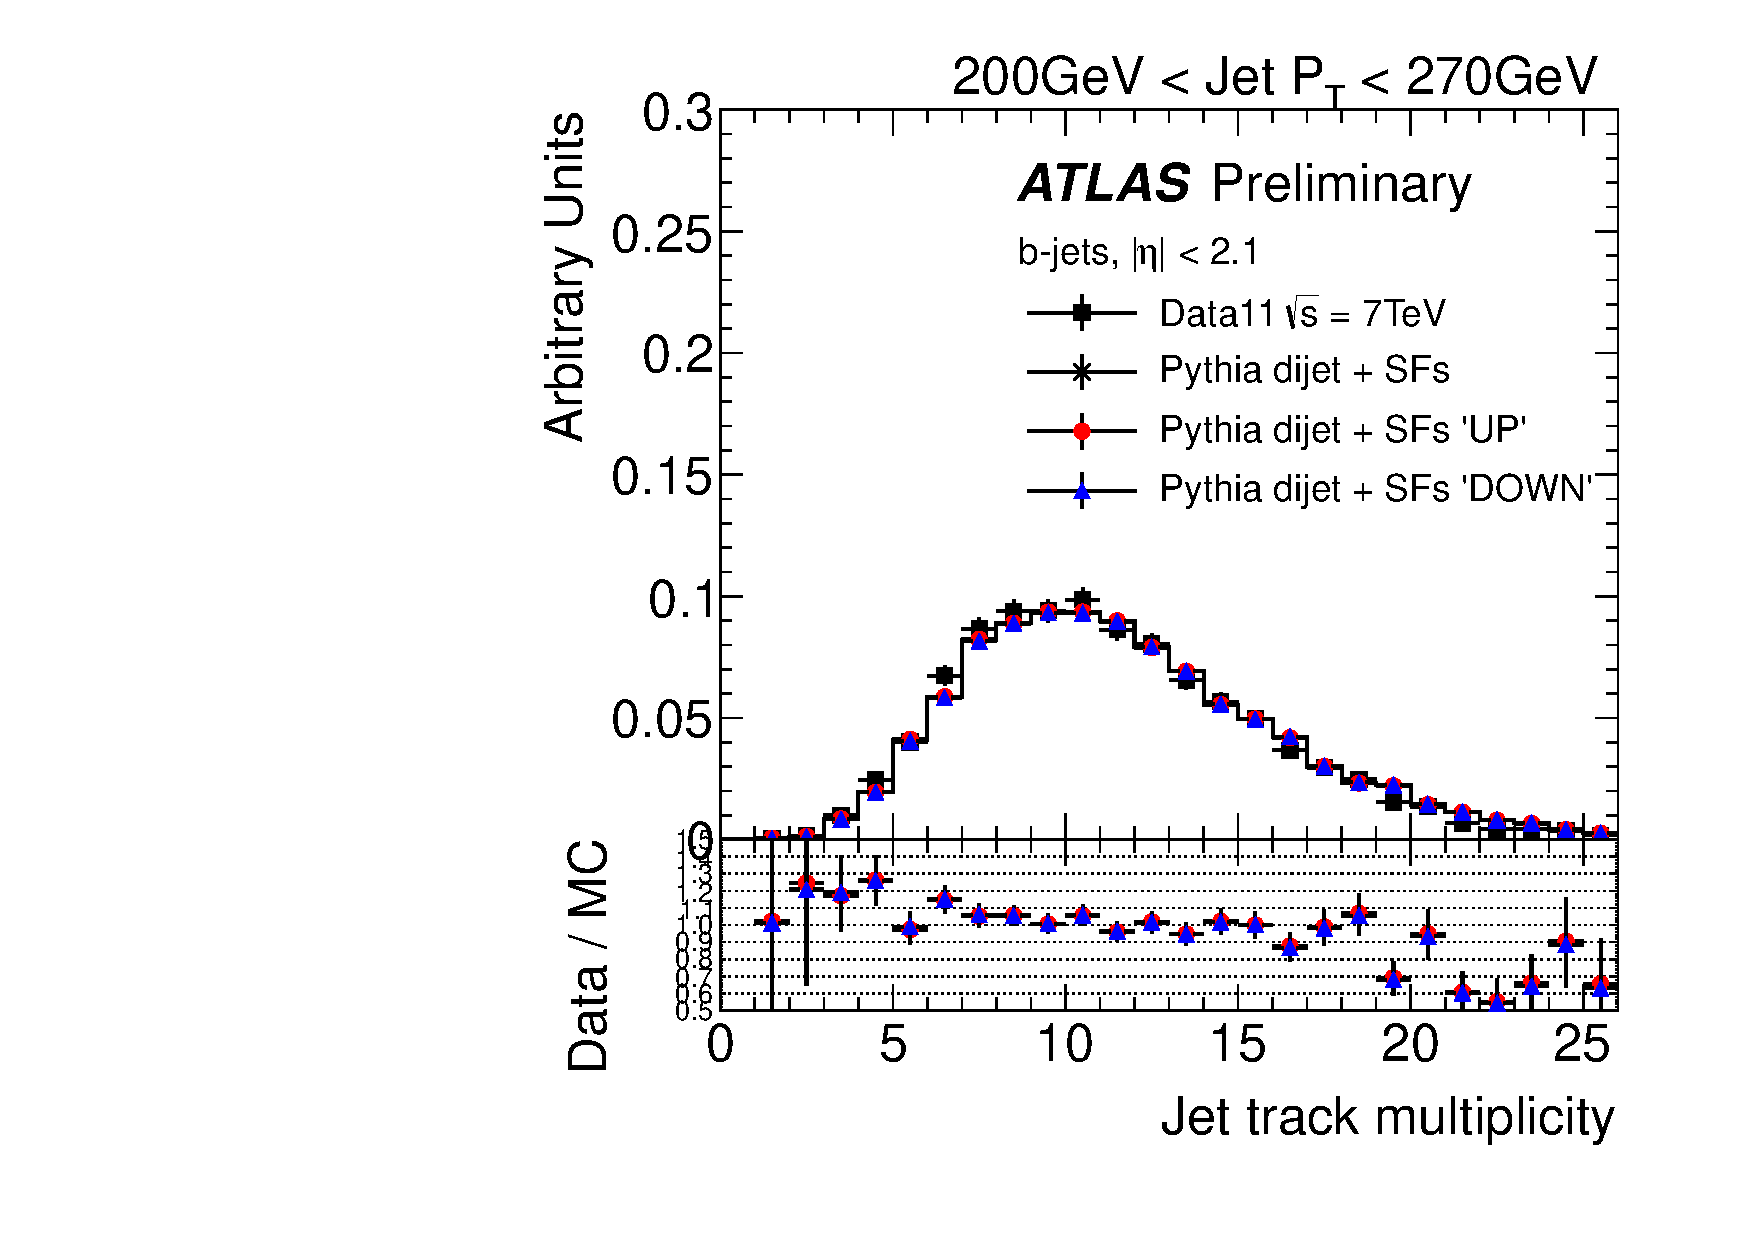
\includegraphics[width=0.49\textwidth]{FIGS/systematics/BTagCalib_DataVarNtrkPT200.pdf}
%%%%%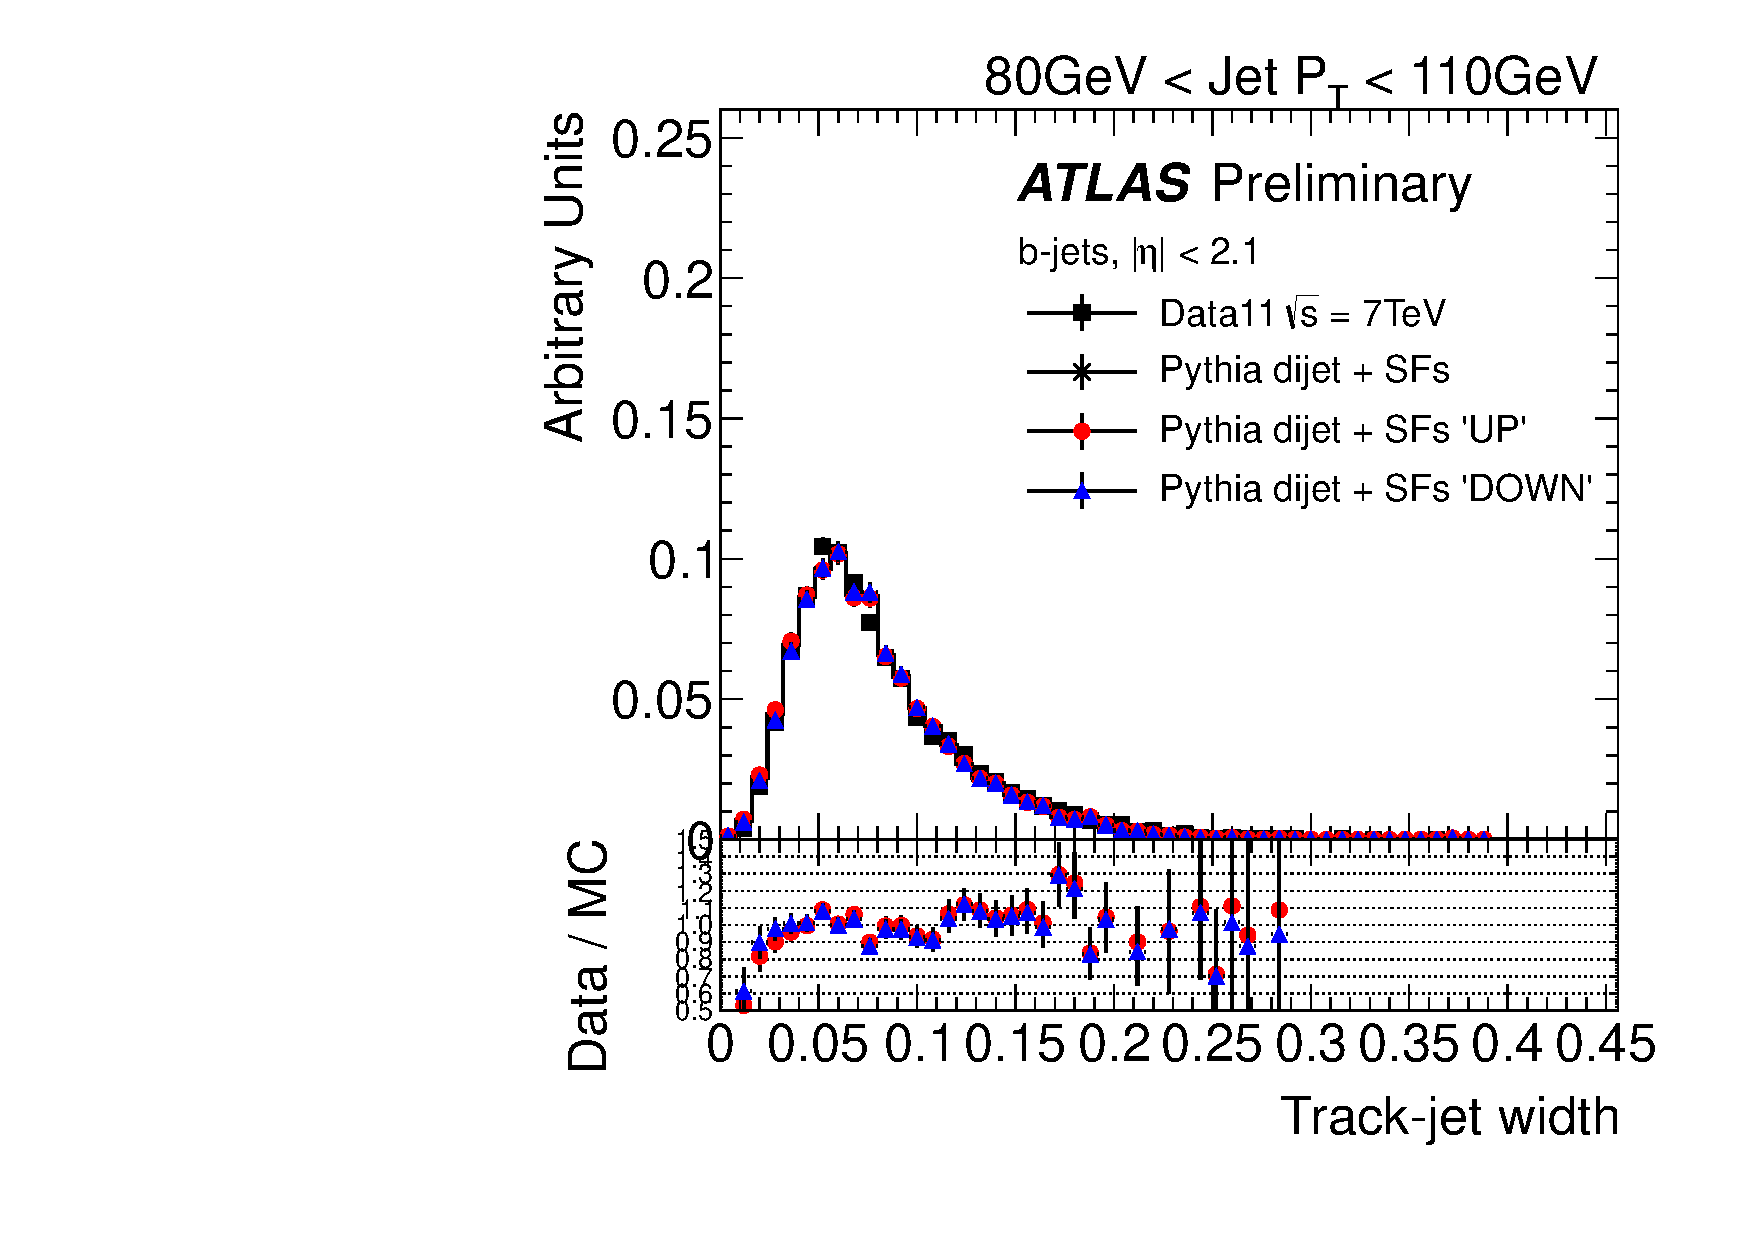
\includegraphics[width=0.49\textwidth]{FIGS/systematics/BTagCalib_DataVarTrkWidthPT080.pdf}
%%%%%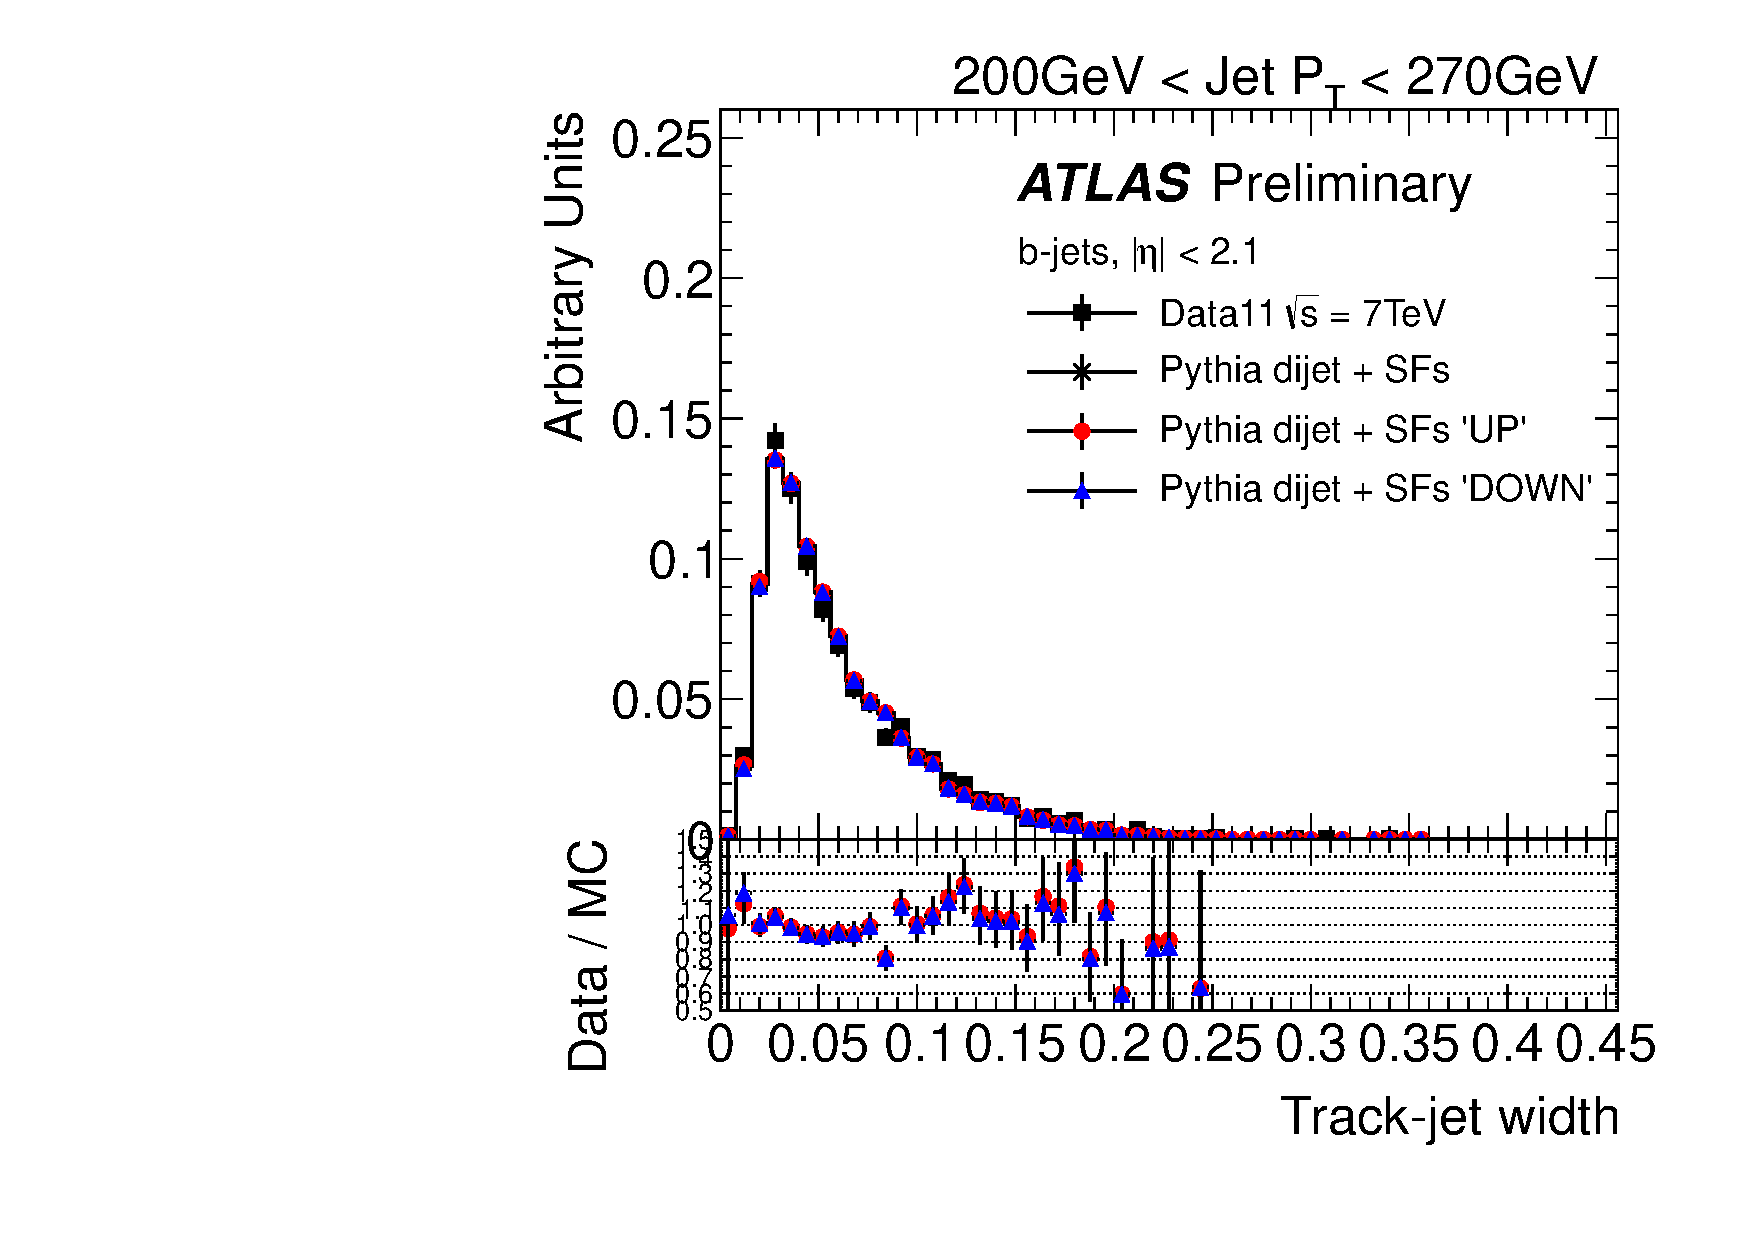
\includegraphics[width=0.49\textwidth]{FIGS/systematics/BTagCalib_DataVarTrkWidthPT200.pdf}
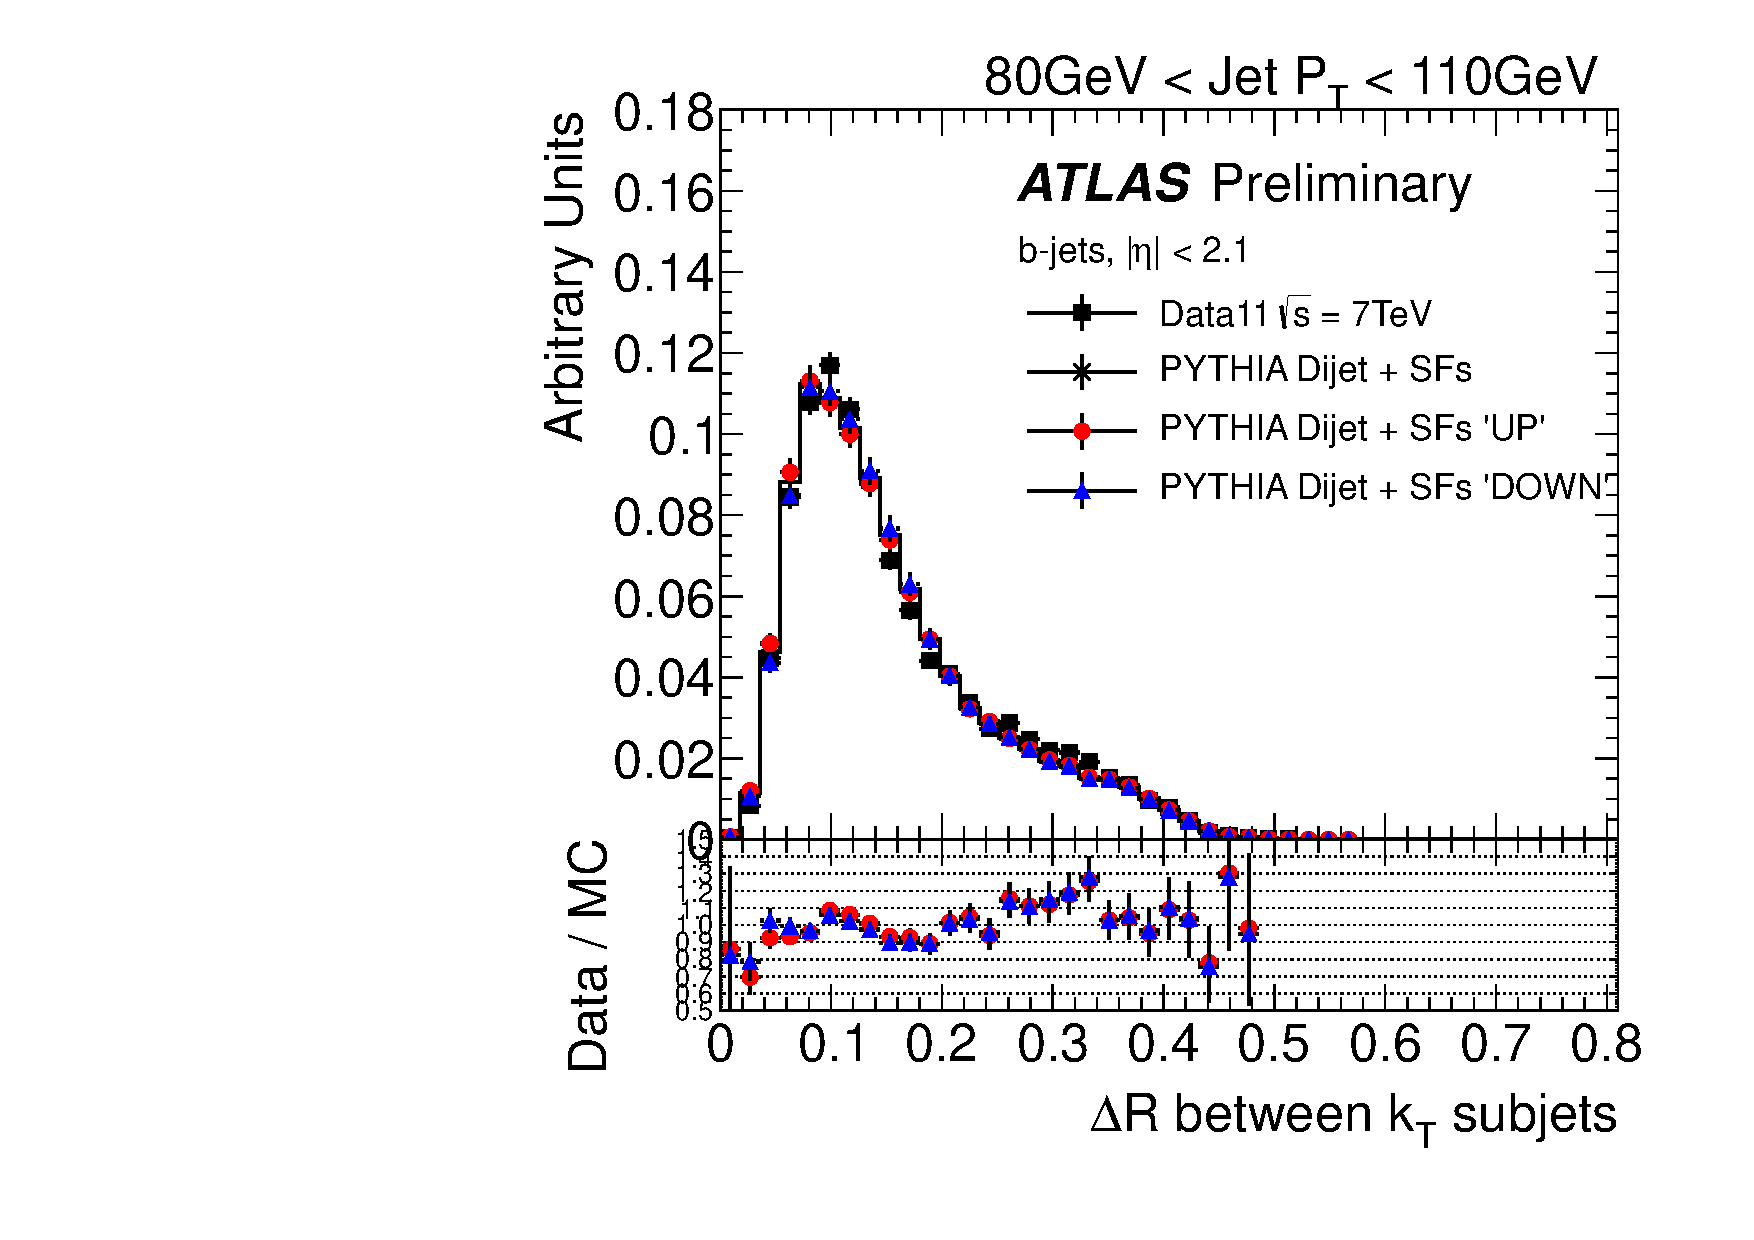
\includegraphics[width=0.49\textwidth]{FIGS/systematics/BTagCalib_DataVarDRktaxisPT080.pdf}
%%%%%%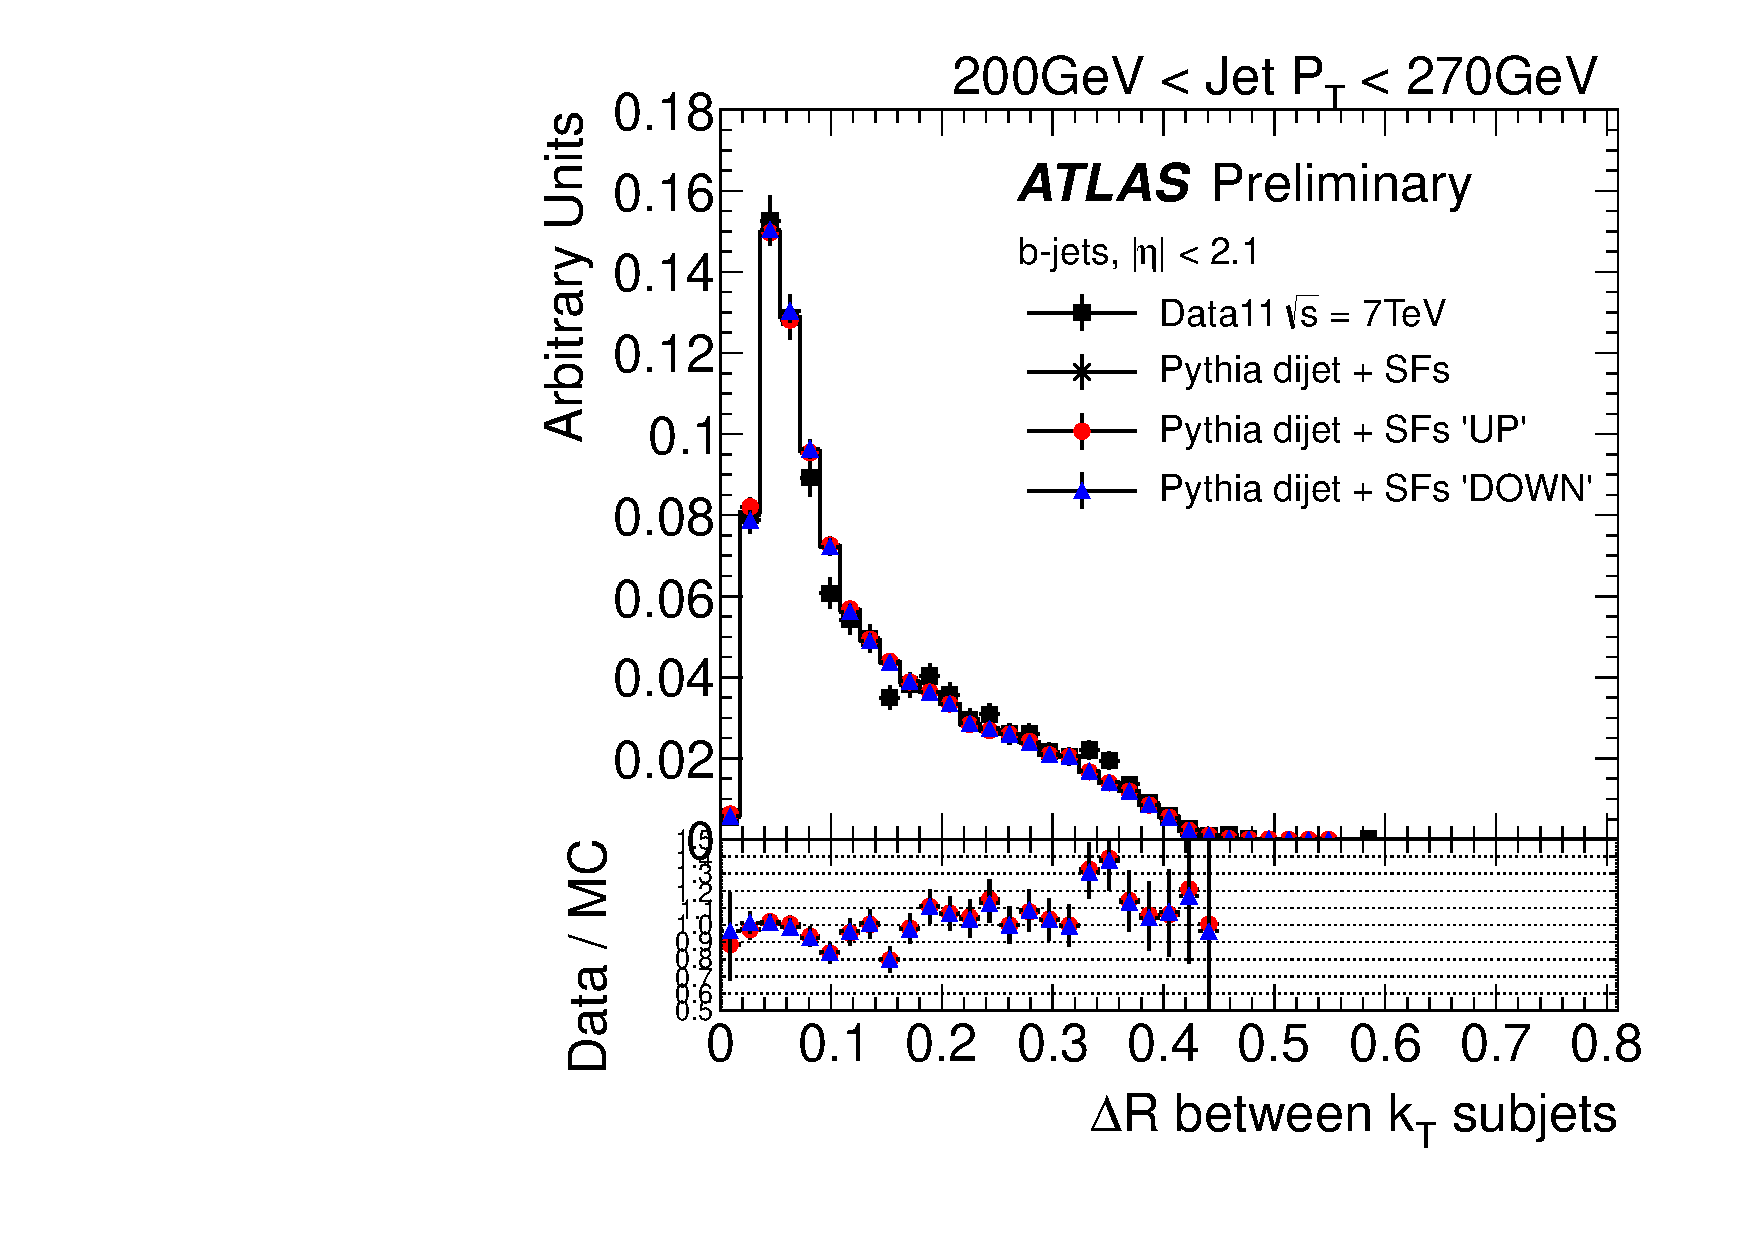
\includegraphics[width=0.49\textwidth]{FIGS/systematics/BTagCalib_DataVarDRktaxisPT200.pdf}
\caption{The effect of a variation in the $b$-tagging Scale Factors on the tracking variables distributions. Scale Factors were varied up (down) by 1-sigma to evaluate the systematic uncertainty from this source. The ratio data over MC is shown for MC {\sc pythia} with SFs varied up (circles) and down (triangles).}
\label{fig:btaggingSFs}
\end{figure}

\begin{figure}[tp]
\centering
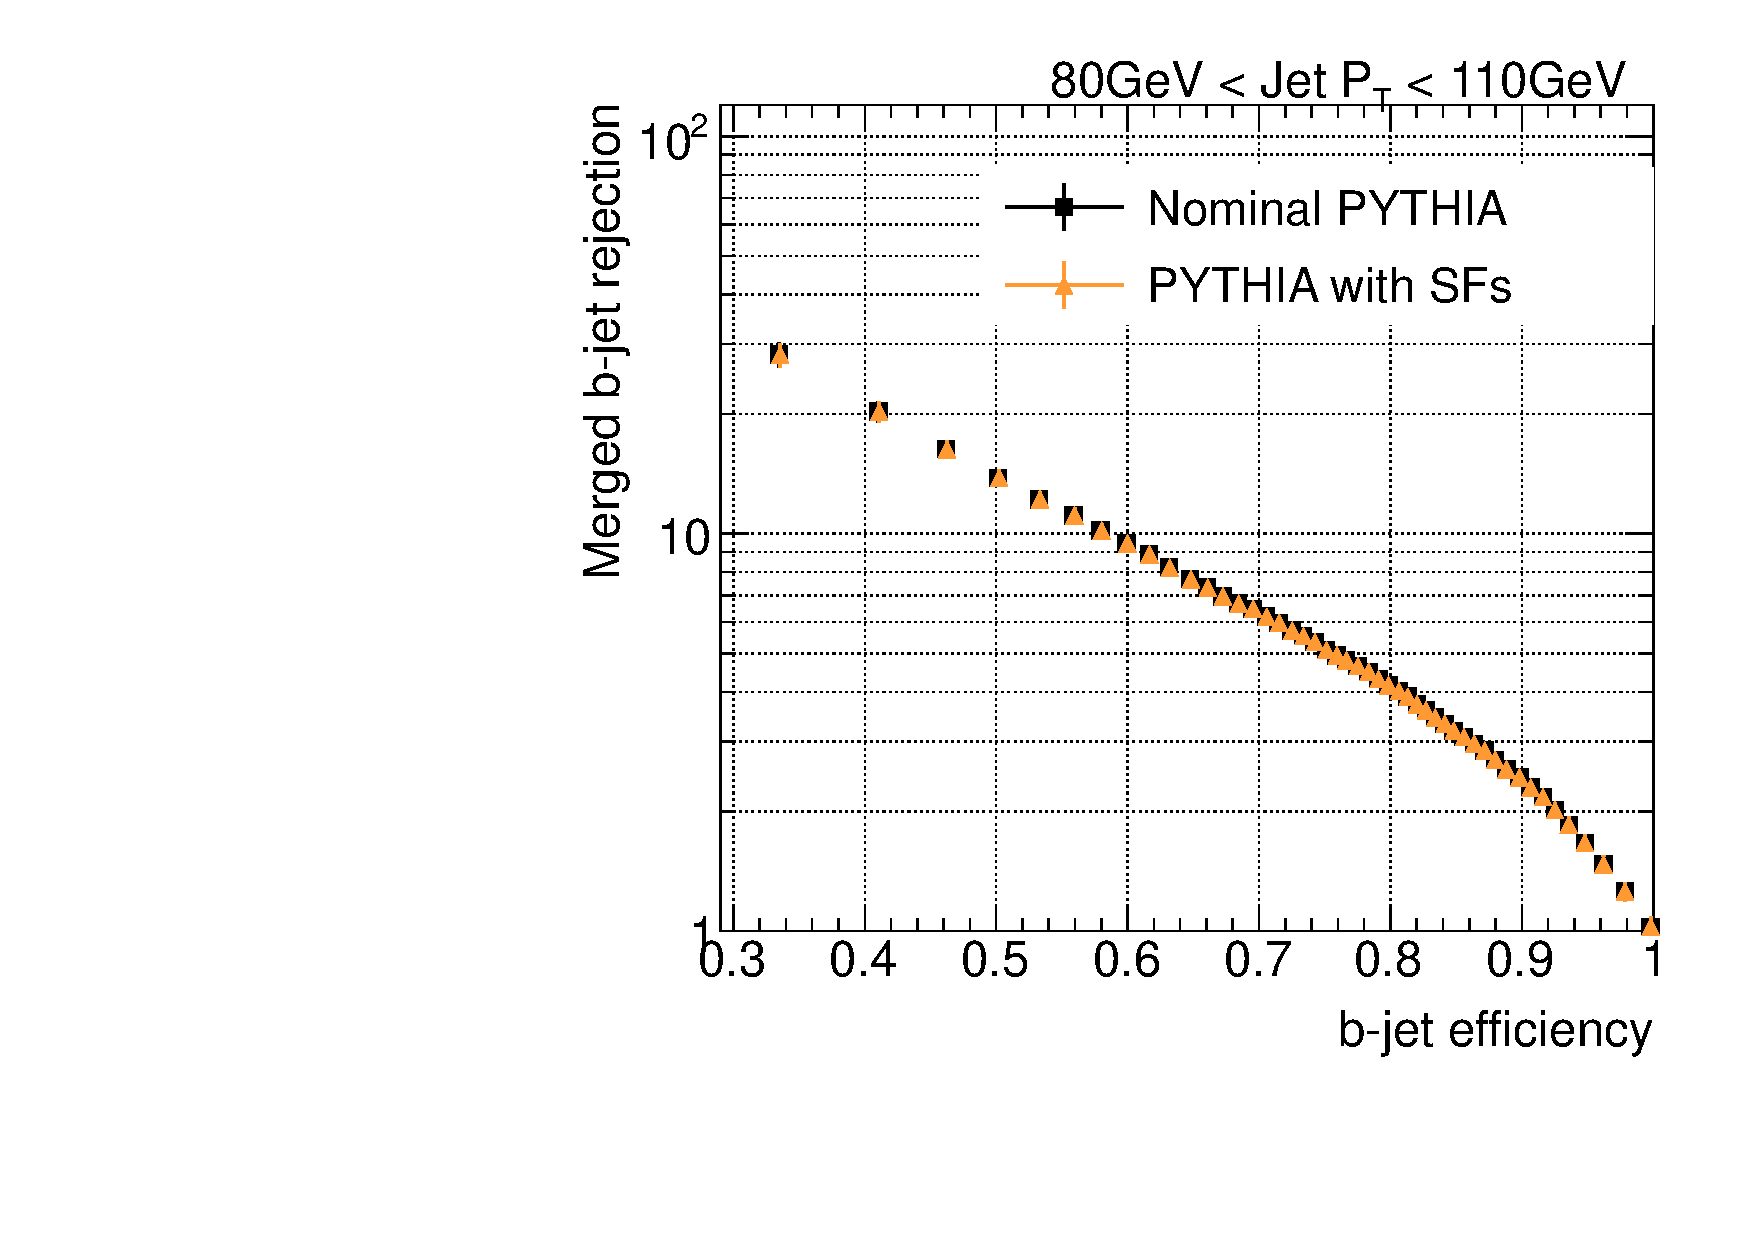
\includegraphics[width=0.49\textwidth]{FIGS/systematics/LlhoodKDE_ISO_BTagCalibTest_rejvseff080.pdf}
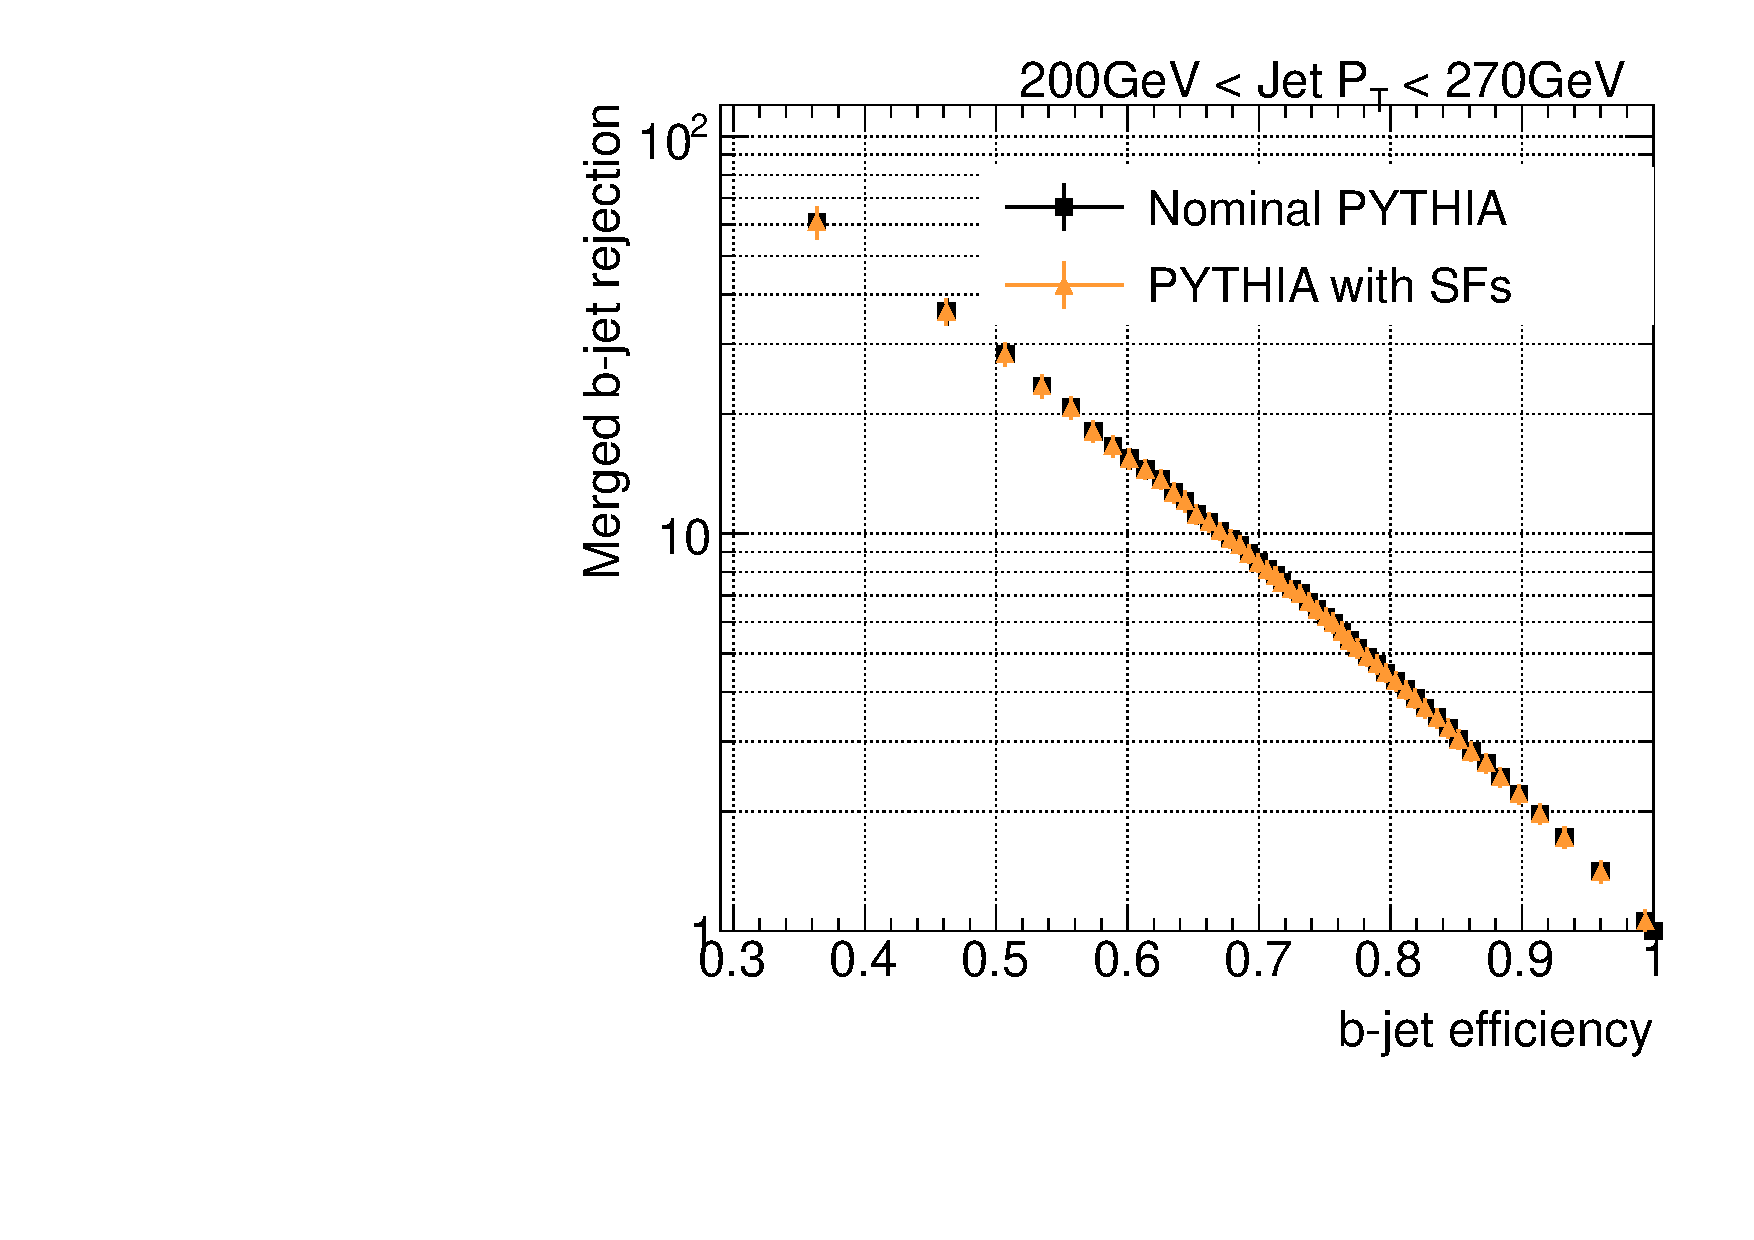
\includegraphics[width=0.49\textwidth]{FIGS/systematics/LlhoodKDE_ISO_BTagCalibTest_rejvseff200.pdf}
\caption{Rejection of merged $b$-jets as a function of single $b$-jet efficiency with and without scale factors as weights.}
\label{fig:btaggingSFsPerf}
\end{figure}



\vspace{5mm}
{ \em III. Track reconstruction efficiency}
\\[3mm]

The track reconstruction efficiency, $\epsilon_{trk}$, parametrised in bins of $\pt$ and $\eta$, is defined as:
%
\begin{equation}
\epsilon_{trk} = \frac{N^{matched}_{rec}(\pt,\eta)}{N_{gen}(\pt,\eta)}
\end{equation}
%
where $N^{matched}_{rec}$ is the number of reconstructed tracks matched to a generated charged particle, and $N_{gen}(\pt,\eta)$ is the number of generated charged particles in that bin\footnote{The matching between a generated particle and a reconstructed track uses a cone-matching algorithm, associating the particle to the track with the smallest $\Delta R$ within a cone of radius 0.15.}.  As the track reconstruction efficiency is determined from MC, the main systematic uncertainty results from the level of agreement between data and MC.  Since charged hadrons are known to suffer from hadronic interactions with the material in the detector, a good description of the material in MC is needed to get a good description of the track reconstruction efficiency.  
%The uncertain knowledge of the material in the inner detector is the main source of systematic uncertainties in the tracking efficiency~\cite{chargemultiplicity}. 
An increase (decrease) in material leads to an increase (decrease) in the number of hadronic interactions, hence to a decrease (increase) in the reconstruction efficiency. 
%This uncertainty arises from the limit in the understanding of the material layout of the Inner Detector. 


The contribution to the tracking reconstruction efficiency systematics of the imperfect description of the detector, in particular the knowledge of the material in the inner tracker, was measured with a data-driven method~\cite{chargemultiplicity}.
The results are given in bins of track $\eta$. For tracks with $p_{\rm{T}}^{\rm{track}} > 500$~MeV the uncertainties are independent of $\pt$:  2\% for $|\eta^{\rm{track}}|<1.3$, 3\% for $1.3<|\eta^{\rm{track}}|<1.9$, 4\% for $1.9<|\eta^{\rm{track}}|<2.1$, 4\% for $2.1<|\eta^{\rm{track}}|<2.3$ and 7\% for $2.3<|\eta^{\rm{track}}|<2.5$. All numbers are relative to the corresponding tracking efficiencies.  

To test the impact of these uncertainties, a fraction of tracks determined from the track efficiency uncertainty was randomly removed.  % following the method in Ref.~\cite{JetMassNote}.%https://cdsweb.cern.ch/record/1344082?ln=en
%https://cdsweb.cern.ch/record/1286839
%http://arxiv.org/abs/1012.5104
The tracking variables were re-calculated and the performance of the nominal likelihood was evaluated in the new sample with worse tracking efficiency. The rejection-efficiency curves %plots, shown in Fig.~\ref{fig:trackefficiency},
 show a small degradation of the performance which is comparable to the statistical uncertainty. The effect is however systematically present over all 16 $\pt$ bin/working points, without a clear $\pt$ dependence. We have thus taken the average over $\pt$, and obtained a global systematic uncertainty of 4\% both for the 50\% and 60\% efficiency working points. The performance comparison is shown in Fig.~\ref{fig:trackefficiency} for two $\pt$ bins. %Similar plots were produced for all other sources of uncertainties considered but are not shown in this note for brevity.

\begin{figure}[tp]
\centering
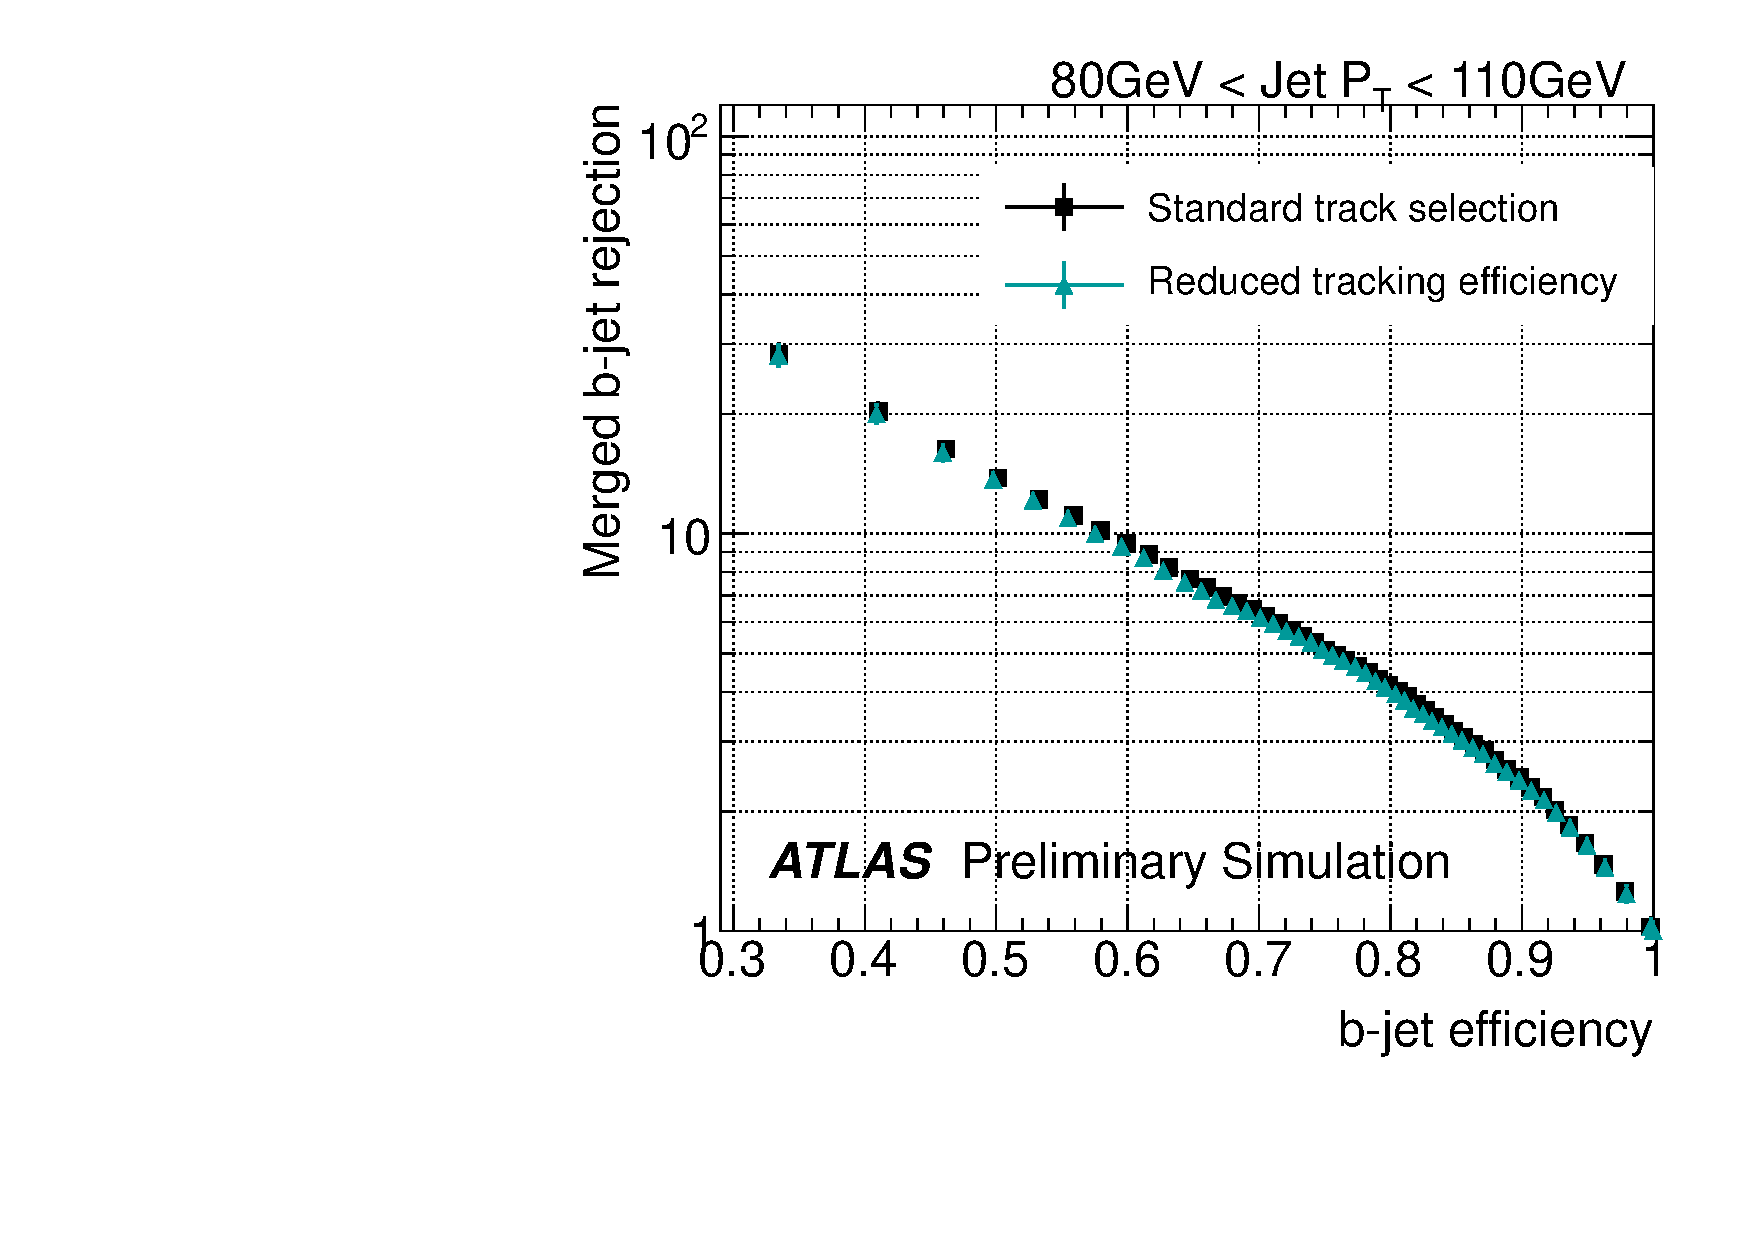
\includegraphics[width=0.49\textwidth]{FIGS/systematics/LlhoodKDE_ISO_TrackingUncertaintyTest_rejvseff080.pdf}
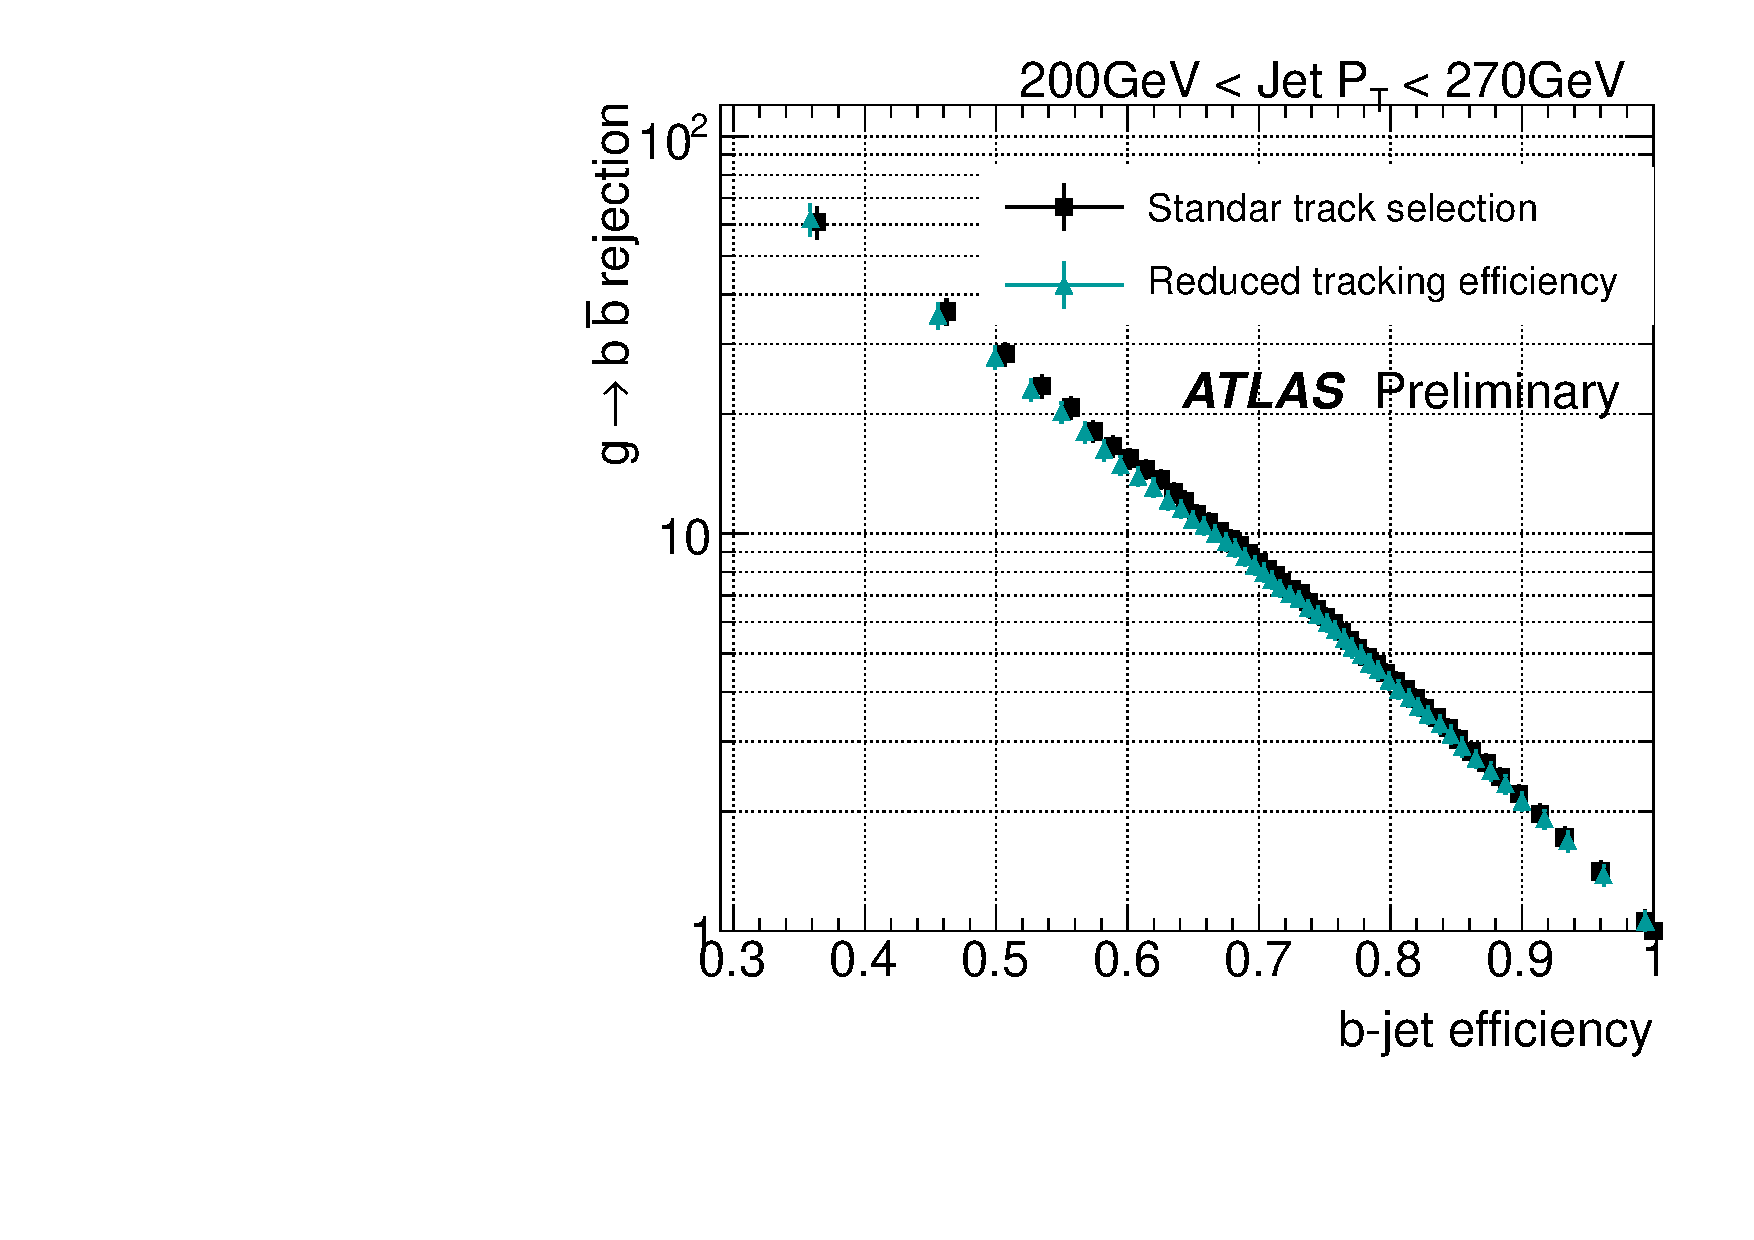
\includegraphics[width=0.49\textwidth]{FIGS/systematics/LlhoodKDE_ISO_TrackingUncertaintyTest_rejvseff200.pdf}
\caption{Rejection of merged $b$-jets as a function of the single $b$-jet efficiency showing shift in likelihood performance caused by a reduction in the tracking efficiency.}
\label{fig:trackefficiency}
\end{figure}

\vspace{3mm}
{\em IV. Track momentum resolution}
\\[3mm]
The knowledge of the track momentum resolution is limited by the precision both in the material description of the Inner Detector and in the mapping of the magnetic field. Its uncertainty propagates to the kinematic variables used in the double $b$-hadron jet tagger. In order to study this effect, track momenta are over-smeared according to the measured resolution uncertainties, before the track selection cuts are applied.  %before computing the rejection. 
The actual smearing is done in 1/$\pt$, which has a gaussian distribution, with an upper bound to the resolution uncertainty given by $\sigma(1/\pt)=0.02/\pt$~\cite{ATLAS-CONF-2010-009}. The effect is found to be negligible. %, see Fig~\ref{fig:trackmomentum}. %with respect to the statistical uncertainty.

%\begin{figure}[tp]
%\centering
%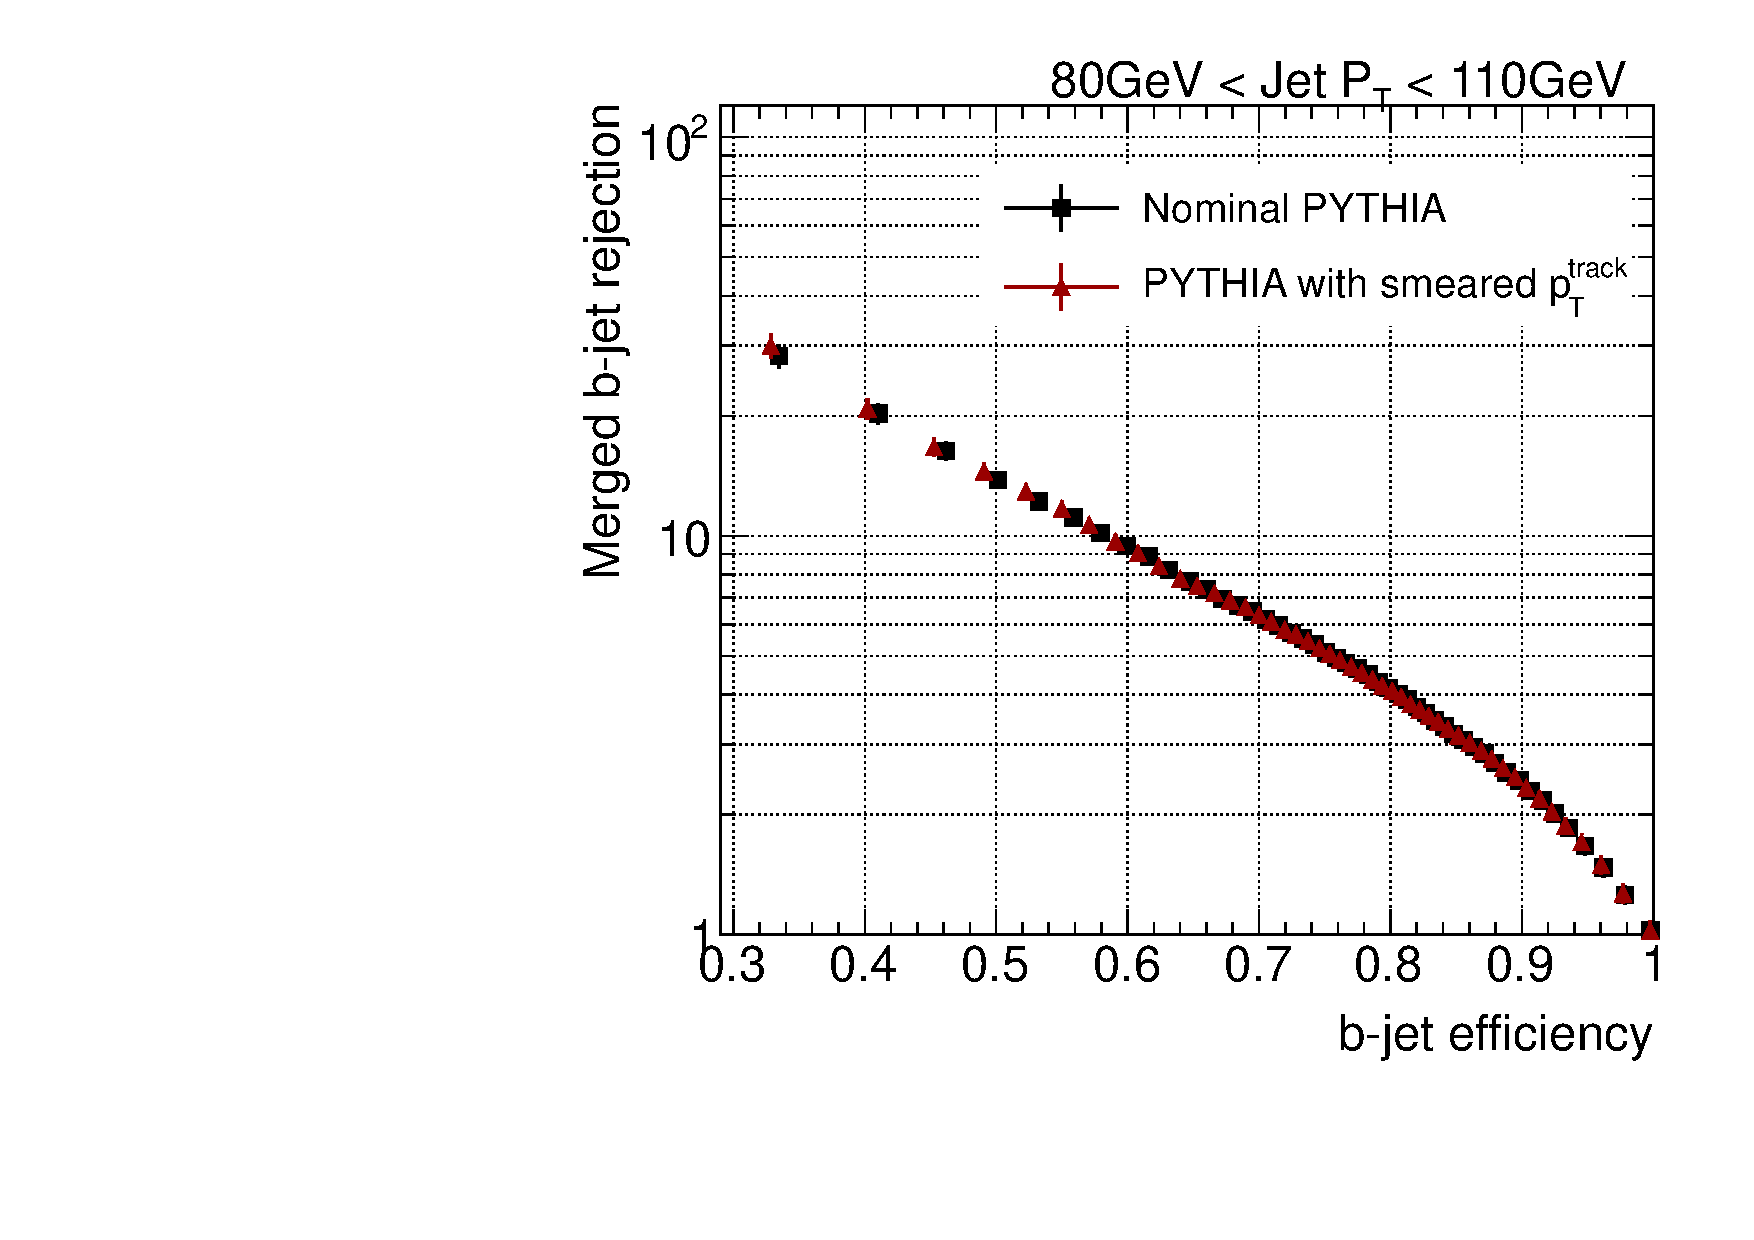
\includegraphics[width=0.49\textwidth]{FIGS/systematics/LlhoodKDE_ISO_TrackMomentumResolution_FIX2Test_rejvseff080.pdf}
%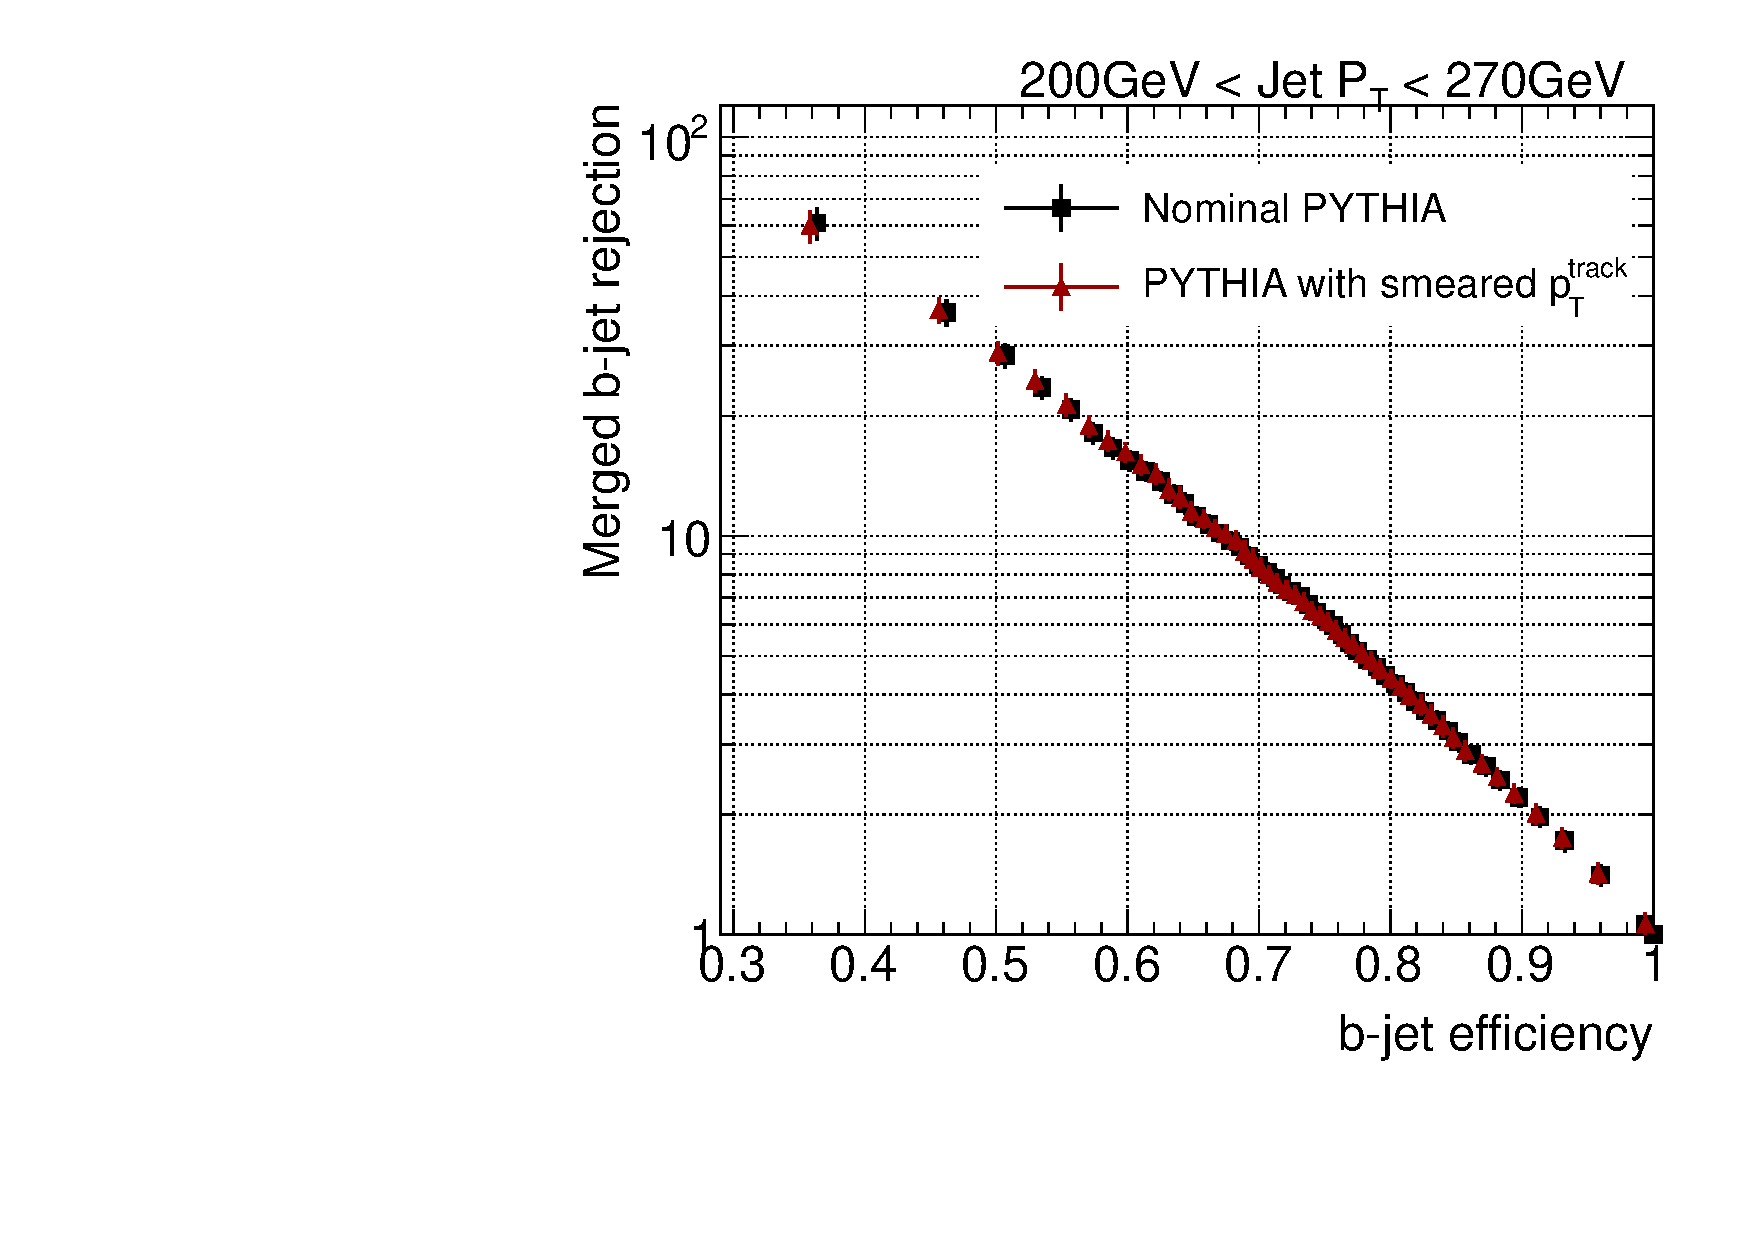
\includegraphics[width=0.49\textwidth]{FIGS/systematics/LlhoodKDE_ISO_TrackMomentumResolution_FIX2Test_rejvseff200.pdf}
%\caption{Rejection of merged $b$-jets as a function of the single $b$-jet efficiency showing the effect of the track momentum resolution uncertainty. It is found to be negligible with respect to the statistical uncertainty. }
%\label{fig:trackmomentum}
%\end{figure}


\vspace{3mm}
{ \em V. Jet energy scale and momentum resolution}
\\[3mm]
The jet energy scale (JES) uncertainty for light jets reconstructed with the anti-$k_t$ algorithm with distance parameter $R=0.4$ and calibrated to the  EM+JES scale is between $\sim$4\% at low $\pt$ and $\sim$2.5\% for jets with  $\pt > $60~GeV in the central region~\cite{JESUncertainty}. In the case of $b$-jets, an additional uncertainty arising from the modelling of the $b$-quark production mechanism and the $b$-quark fragmentation was determined from systematic variations of the Monte Carlo simulation. % and validated up to $\sim$3\% in 2011 data and MC. 
The resulting fractional additional JES uncertainty for $b$-jets has an upper bound of 2\% for jets with $\pt \leq$100~GeV and it is below 1\% for higher $\pt$ jets. To obtain the overall $b$-jet uncertainty this needs to be added in quadrature to the light JES uncertainty. 

The systematic uncertainty originating from the jet energy scale is obtained by scaling the $\pt$ of each jet in the simulation up and down by one standard deviation according to the uncertainty of the JES.  The result is shown in Fig.~\ref{fig:jetresolution}a for a medium $\pt$ bin. The effect on the likelihood performance is an average variation of 5\% for the 50\% and 60\% efficiency working points. 

The jet momentum resolution was measured for 2011 data and found to be in agreement with the predictions from the {\sc pythia}-based simulation~\cite{JER2011}. The precision of this measurement, determined in $\pt$ and $\eta$ bins, is typically 10\%.
The systematic uncertainty due to the calorimeter jet $\pt$ resolution was estimated by over-smearing the jet $4$-momentum in the simulated data, without changing jet $\eta$ or $\phi$ angles. The performance, shown in Fig.~\ref{fig:jetresolution}b, is found to globally decrease by  % 6\%, 
5\%, without a particular $\pt$ dependence.


\begin{figure}[tp]
\centering
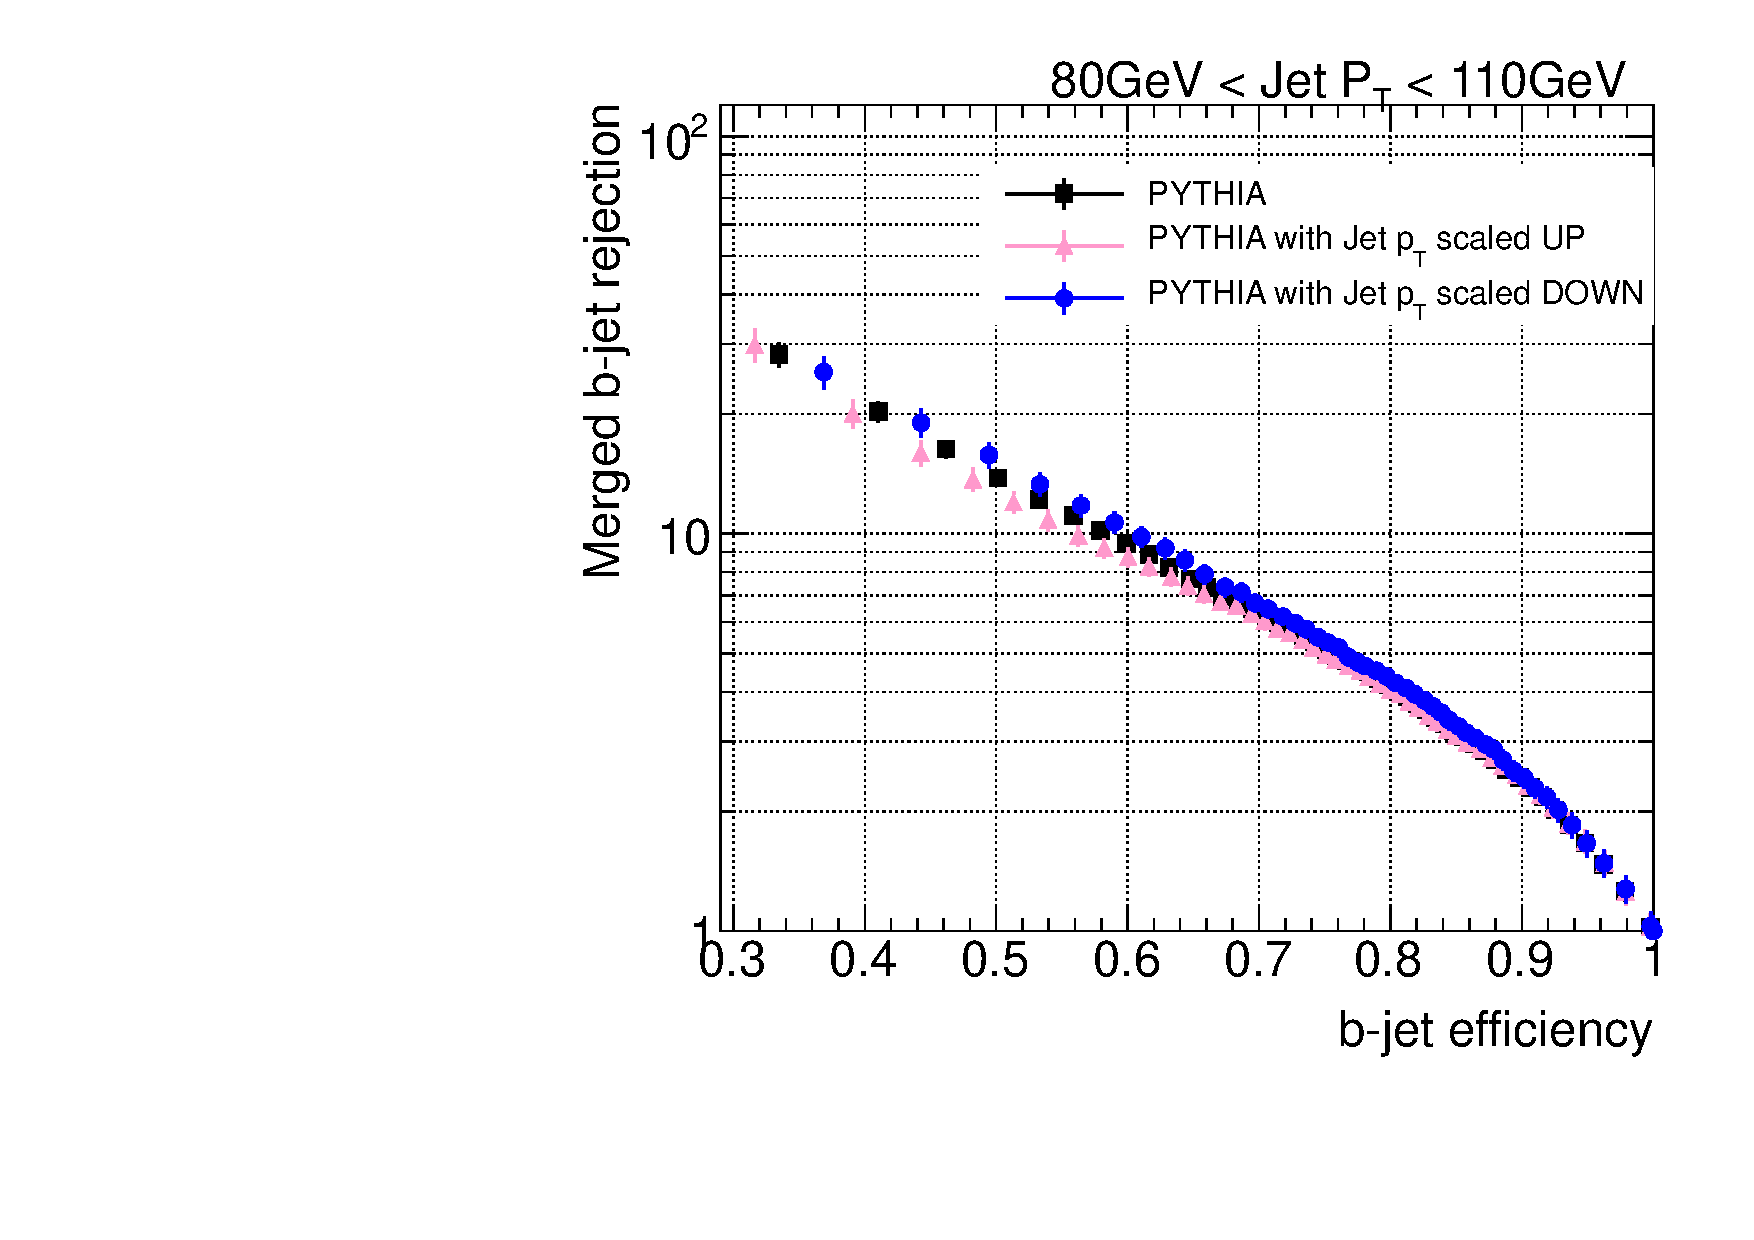
\includegraphics[width=0.49\textwidth]{FIGS/systematics/LlhoodKDE_ISO_JESUncertaintyTest_rejvseff080.pdf}
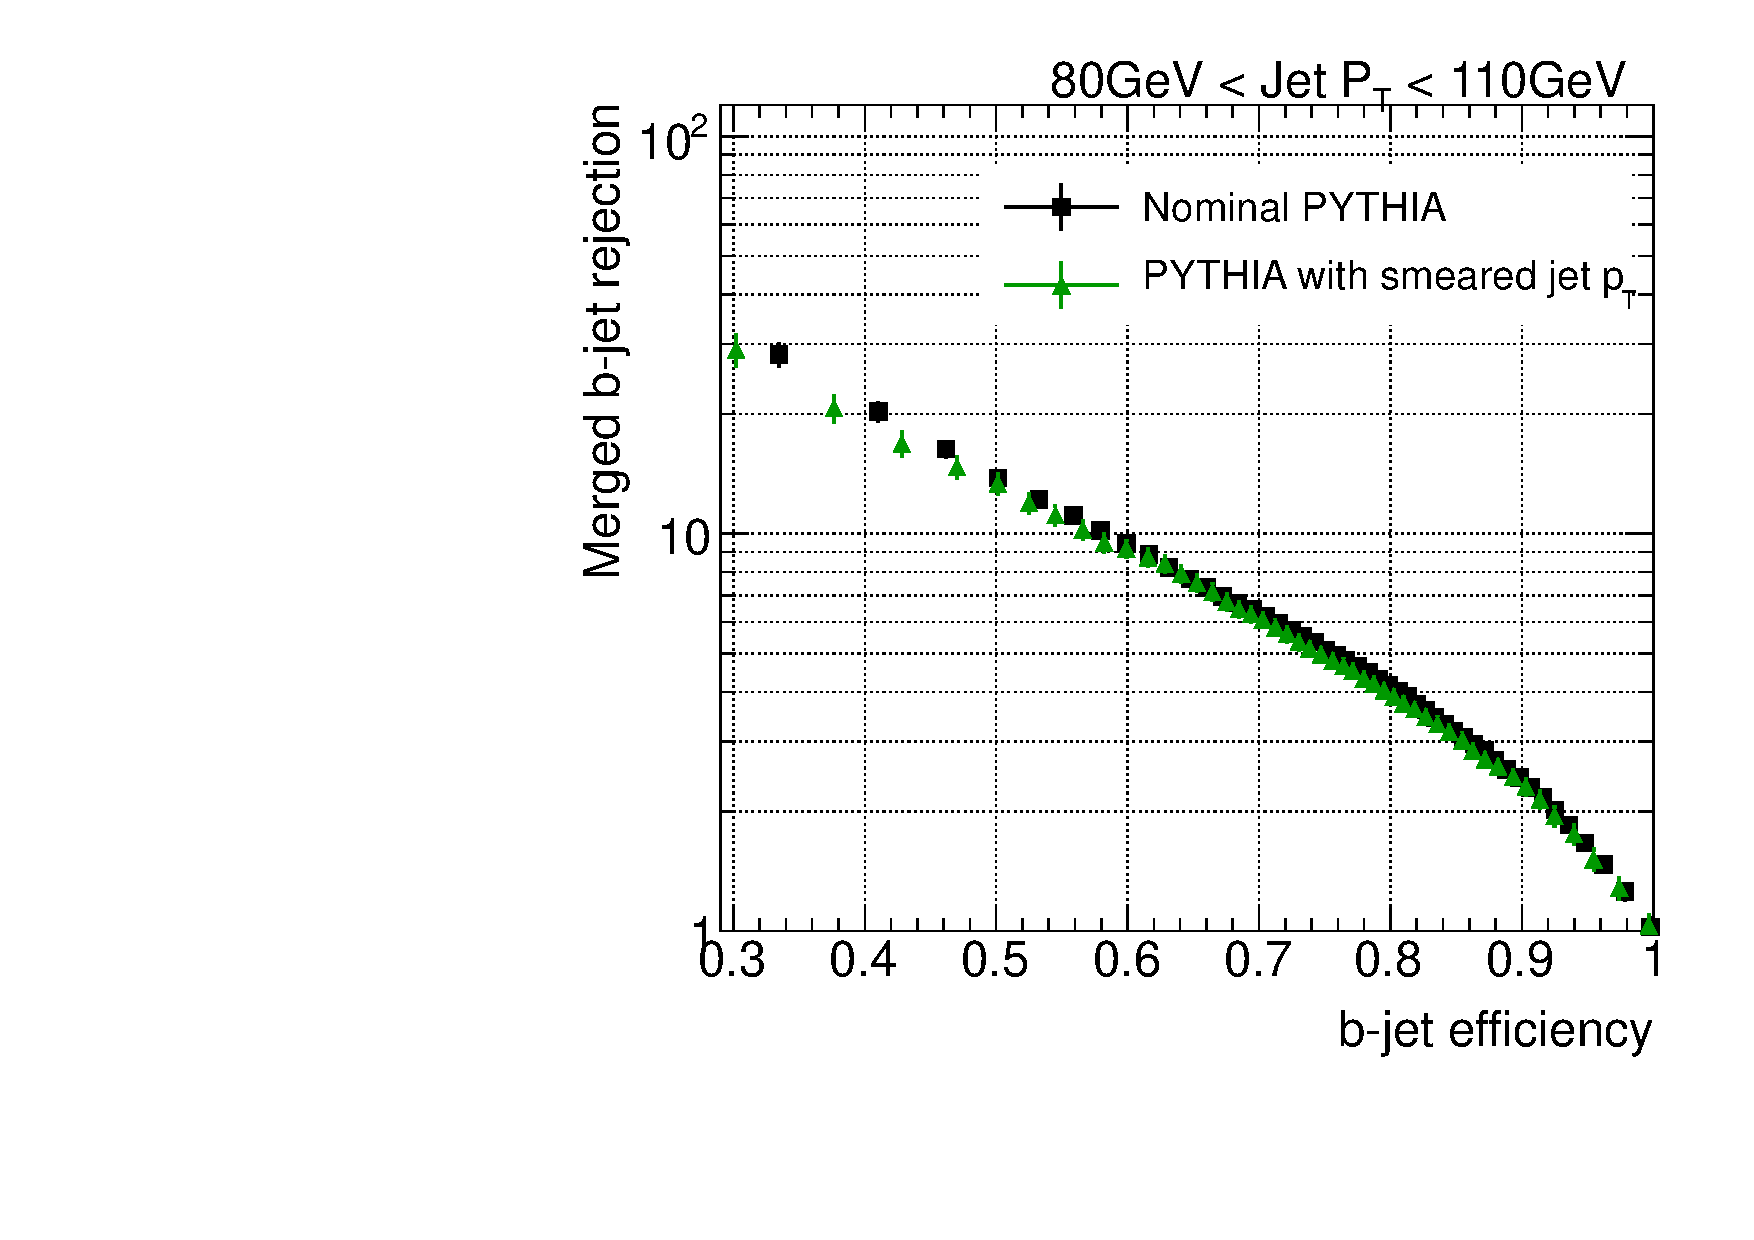
\includegraphics[width=0.49\textwidth]{FIGS/systematics/LlhoodKDE_ISO_SmearedJetPt_FIXEDBUGTest_rejvseff080.pdf}
\caption{Rejection of merged $b$-jets as a function of single $b$-jet efficiency for (a) jets with smeared $\pt$ and (b) for jets with varied energy scale compared to nominal.}
\label{fig:jetresolution}
\end{figure}


%\vspace{3mm}
%{ \em VI. Jet energy scale for heavy flavour jets}
%\\[3mm]
%%%The calorimeter jet response uncertainties for $b$-jets was evaluated using single hadron response measurements in MC samples of inclusive dijet and $b \bar{b}$ dijet events. 
%The jet energy scale (JES) uncertainty for light jets reconstructed with the anti-$k_t$ algorithm with distance parameter $R=0.4$ and calibrated to the  EM+JES scale is between $\sim$4\% at low $\pt$ and $\sim$2.5\% for jets with  $\pt > $60~GeV in the central region~\cite{bjetJES}. In the case of $b$-jets, and additional uncertainty arising from the modelling of the $b$-quark production mechanism and the $b$-quark fragmentation was determined from systematic variations of the Monte Carlo simulation. % and validated up to $\sim$3\% in 2011 data and MC. 
%The resulting fractional additional JES uncertainty for $b$-jets has an upper bound of 2\% for jets with $\pt \leq$100~GeV and it is below 1\% for higher $\pt$ jets. To obtain the overall $b$-jet uncertainty this needs to be added in quadrature to the light JES uncertainty. 

%The systematic uncertainty originating from the jet energy scale is obtained by scaling the $\pt$ of each jet in the simulation up and down by one standard deviation according to the uncertainty of the JES.  The result is shown in Fig.~\ref{fig:jesuncertainty}. The effect on the likelihood performance is an average variation of 5\% for the 50\% and 60\% efficiency working points. 


%\begin{figure}[tp]
%\centering
%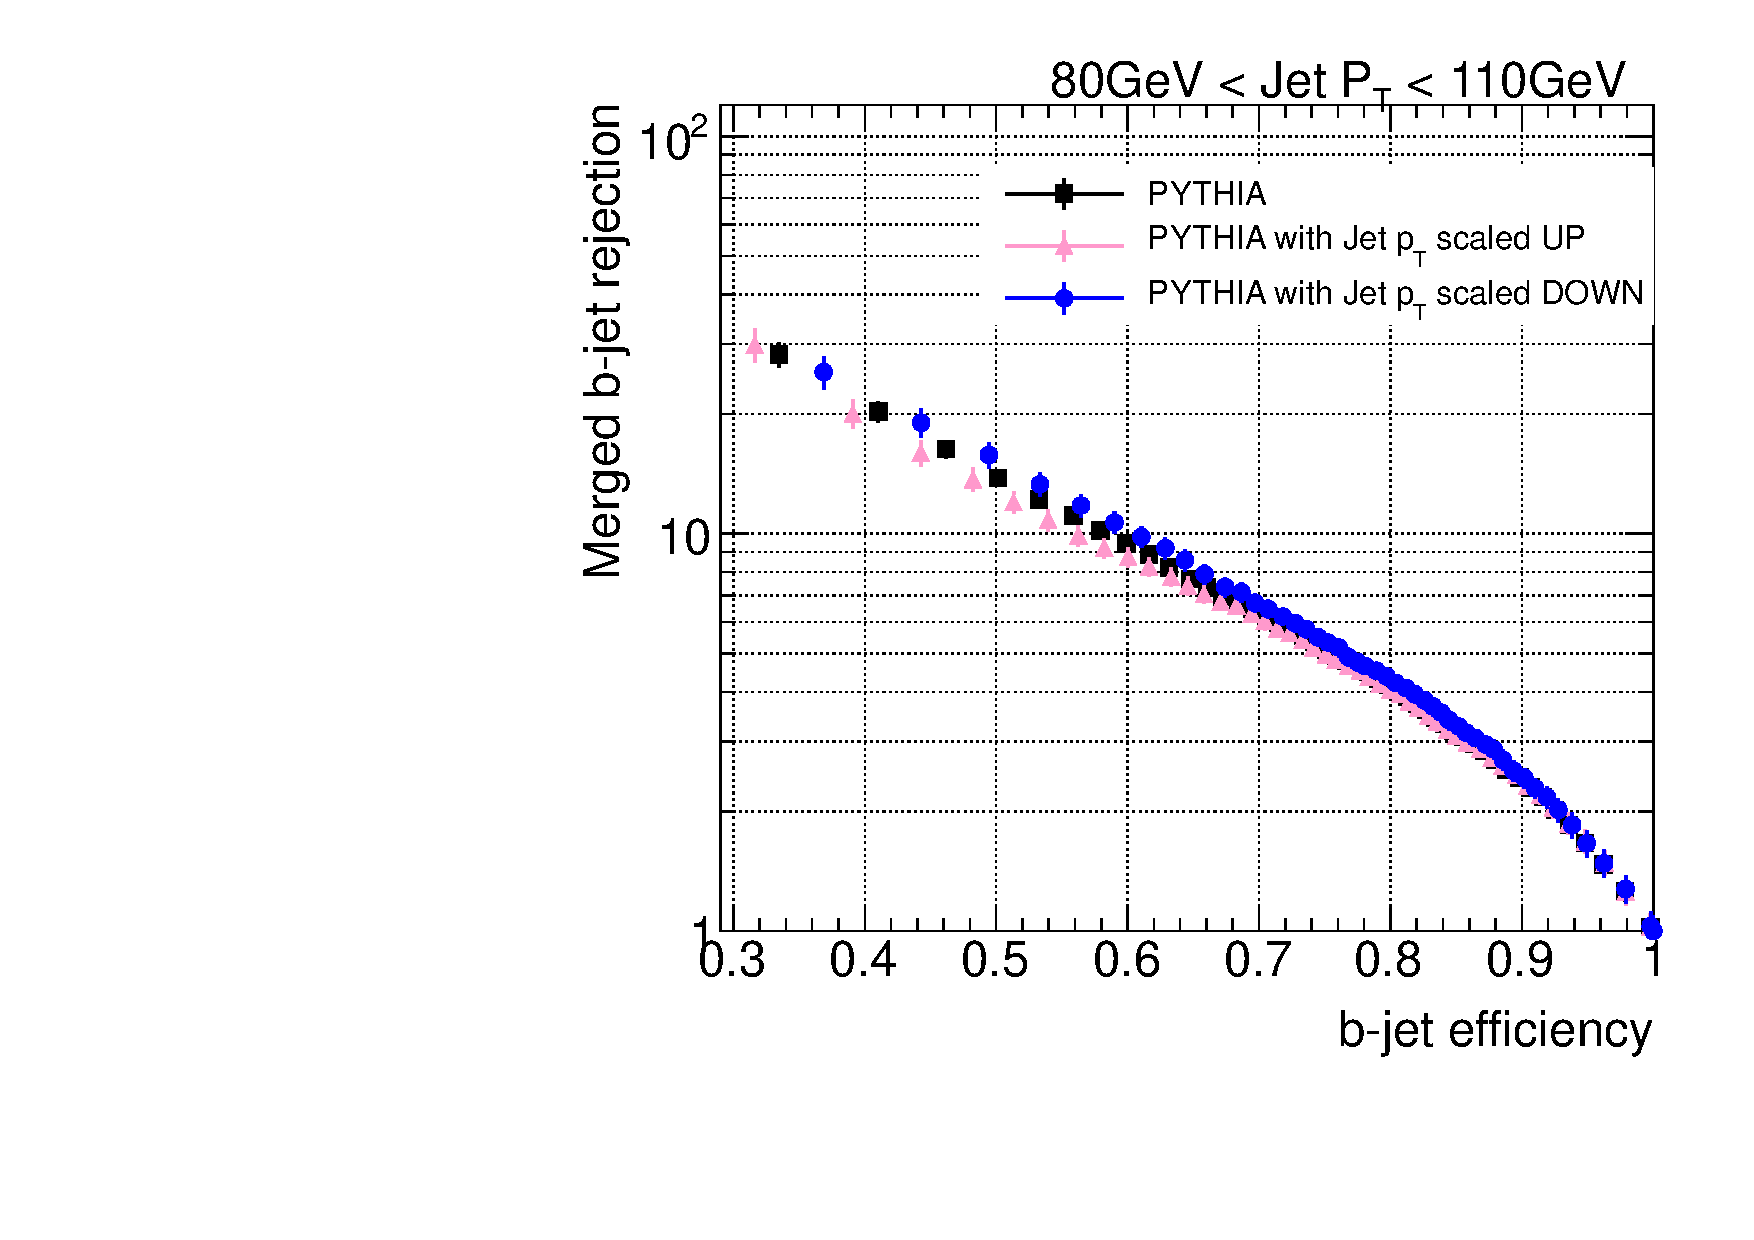
\includegraphics[width=0.49\textwidth]{FIGS/systematics/LlhoodKDE_ISO_JESUncertaintyTest_rejvseff080.pdf}
%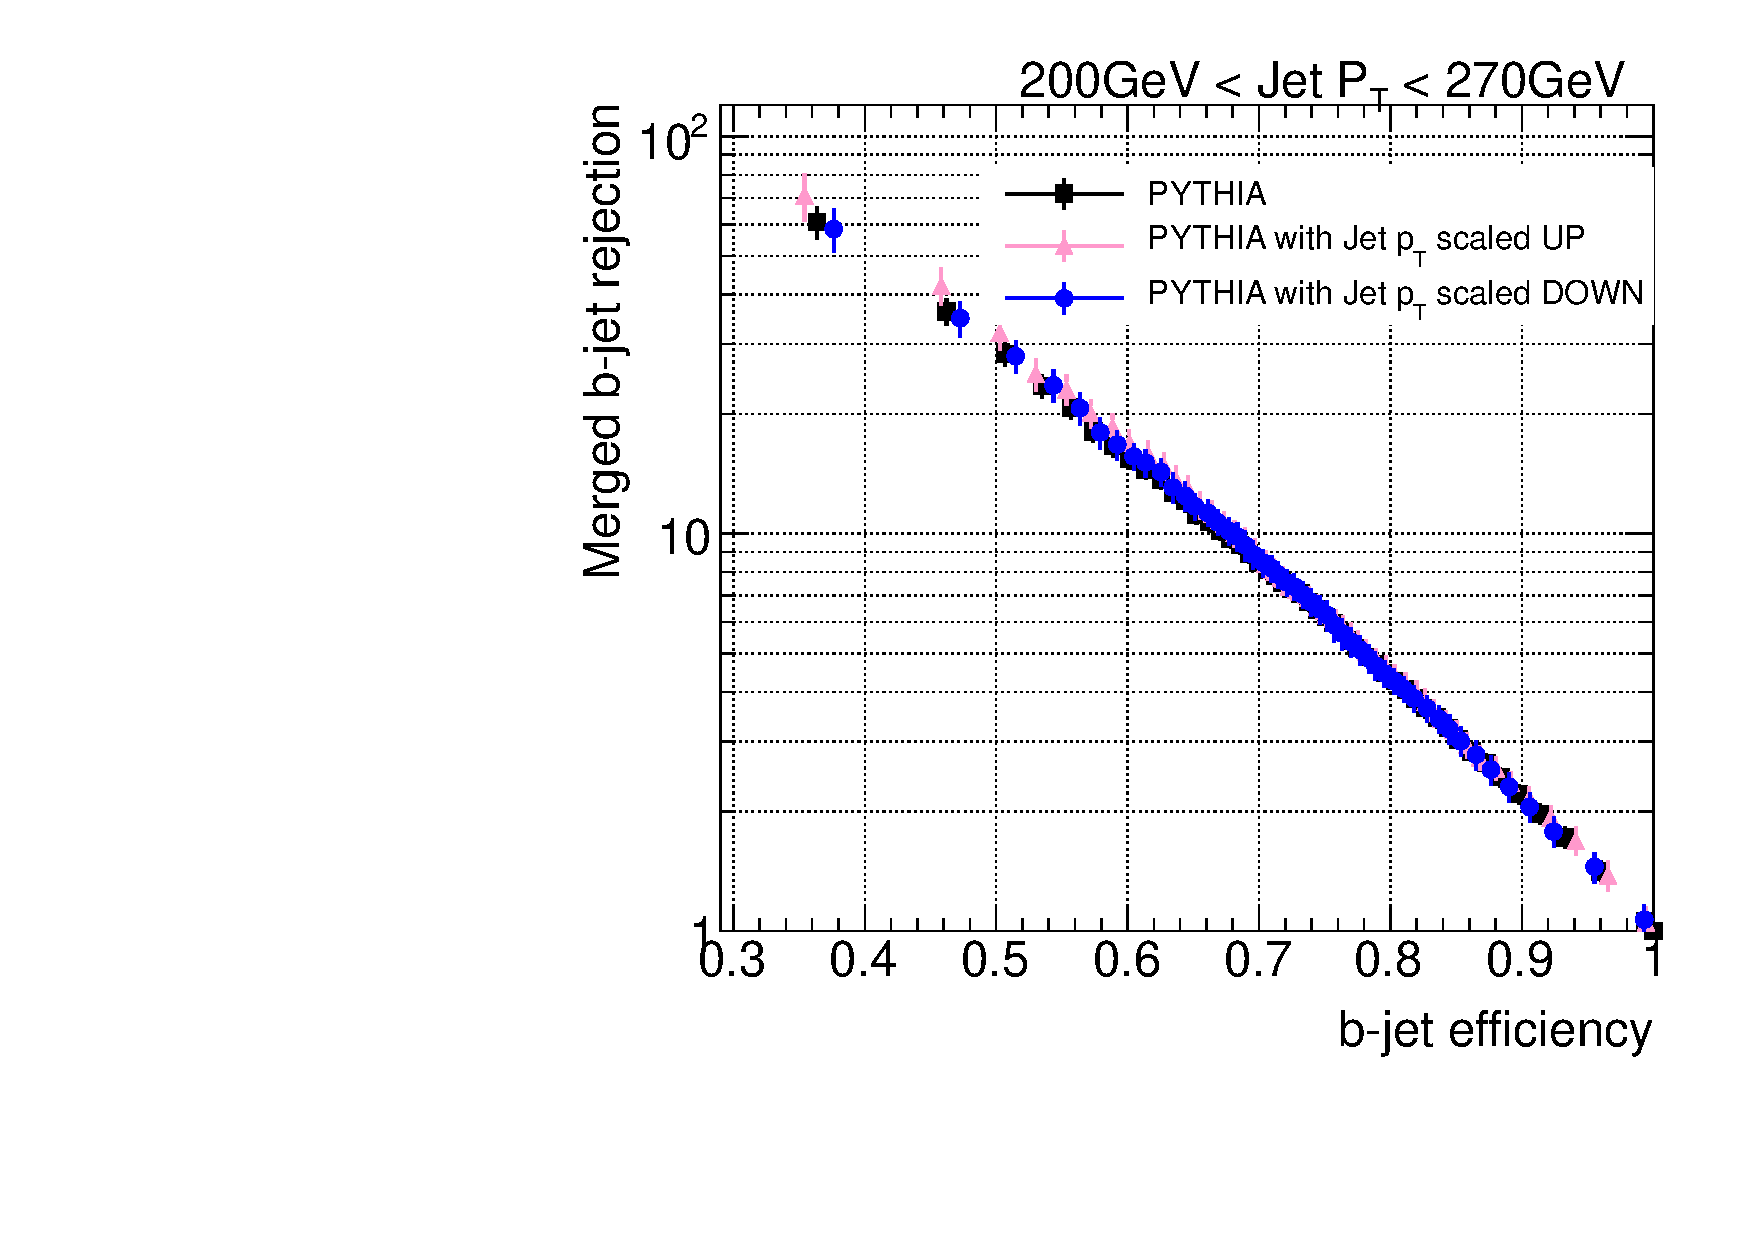
\includegraphics[width=0.49\textwidth]{FIGS/systematics/LlhoodKDE_ISO_JESUncertaintyTest_rejvseff200.pdf}
%\caption{Rejection of merged $b$-jets as a function of single $b$-jet efficiency for jets with varied energy scale compared to nominal.}
%\label{fig:jesuncertainty}
%\end{figure}


\vspace{3mm}
The different contributions to the systematic uncertainty on the merged $b$-jet rejection are summarized in Table~\ref{tb:systematics}.
\begin{table}[!hbt] %[h]
\renewcommand{\arraystretch}{1.2}
\centering
\begin{tabular}{ | c | c |}
\hline
  ~~~~~~~Systematic source~~~~~~~ &~~Uncertainty~~\\ \hline
  pile-up          &  2\%     \\ 
  $b$-tagging efficiency     &  neglible     \\ 
  track reconstruction efficiency  &    4\%        \\ 
  track $\pt$ resolution &  neglible     \\
  jet $\pt$ resolution  &    5\%        \\  
  jet energy scale  &    5\%        \\ \hline 
\end{tabular}
\caption{Systematic uncertainties in the merged $b$-jet rejection (common to both the 50\% and the 60\% efficiency working points).}
\label{tb:systematics}
\end{table}


Although the likelihood training was peformed in EM+JES calibrated jets, the performance of the tagger was also evaluated in jets calibrated with the LC+JES scheme, described in Section~\ref{sec:calib}.  A small degradation of the performance is observed, but comparable with the statistical uncertanties. A comparison of the performances is shown in Fig.~\ref{fig:LCJES} for two $\pt$ bins, representative of the jet momentum range covered. 

\begin{figure}[tp]
\centering
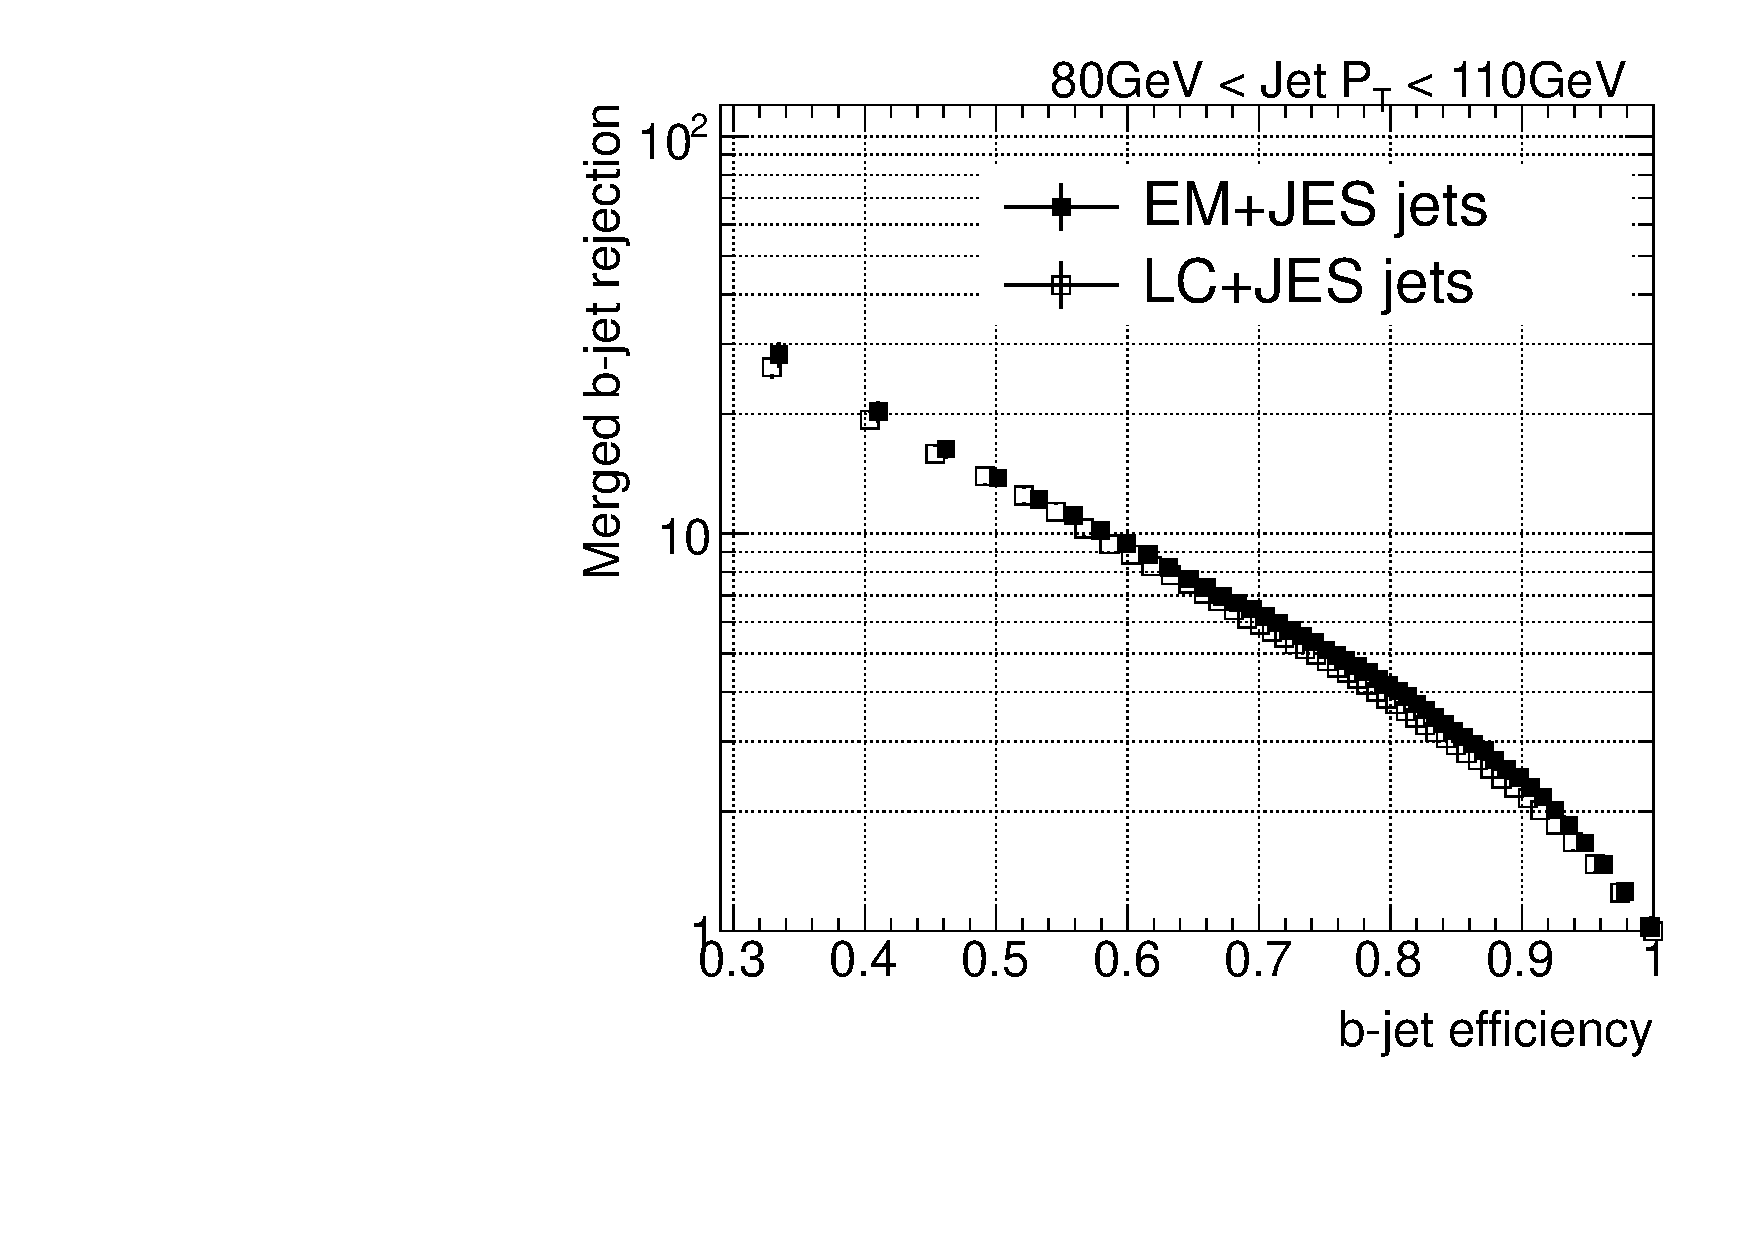
\includegraphics[width=0.49\textwidth]{FIGS/systematics/LlhoodKDE_ISO_LCcalibTest_rejvseff080.pdf}
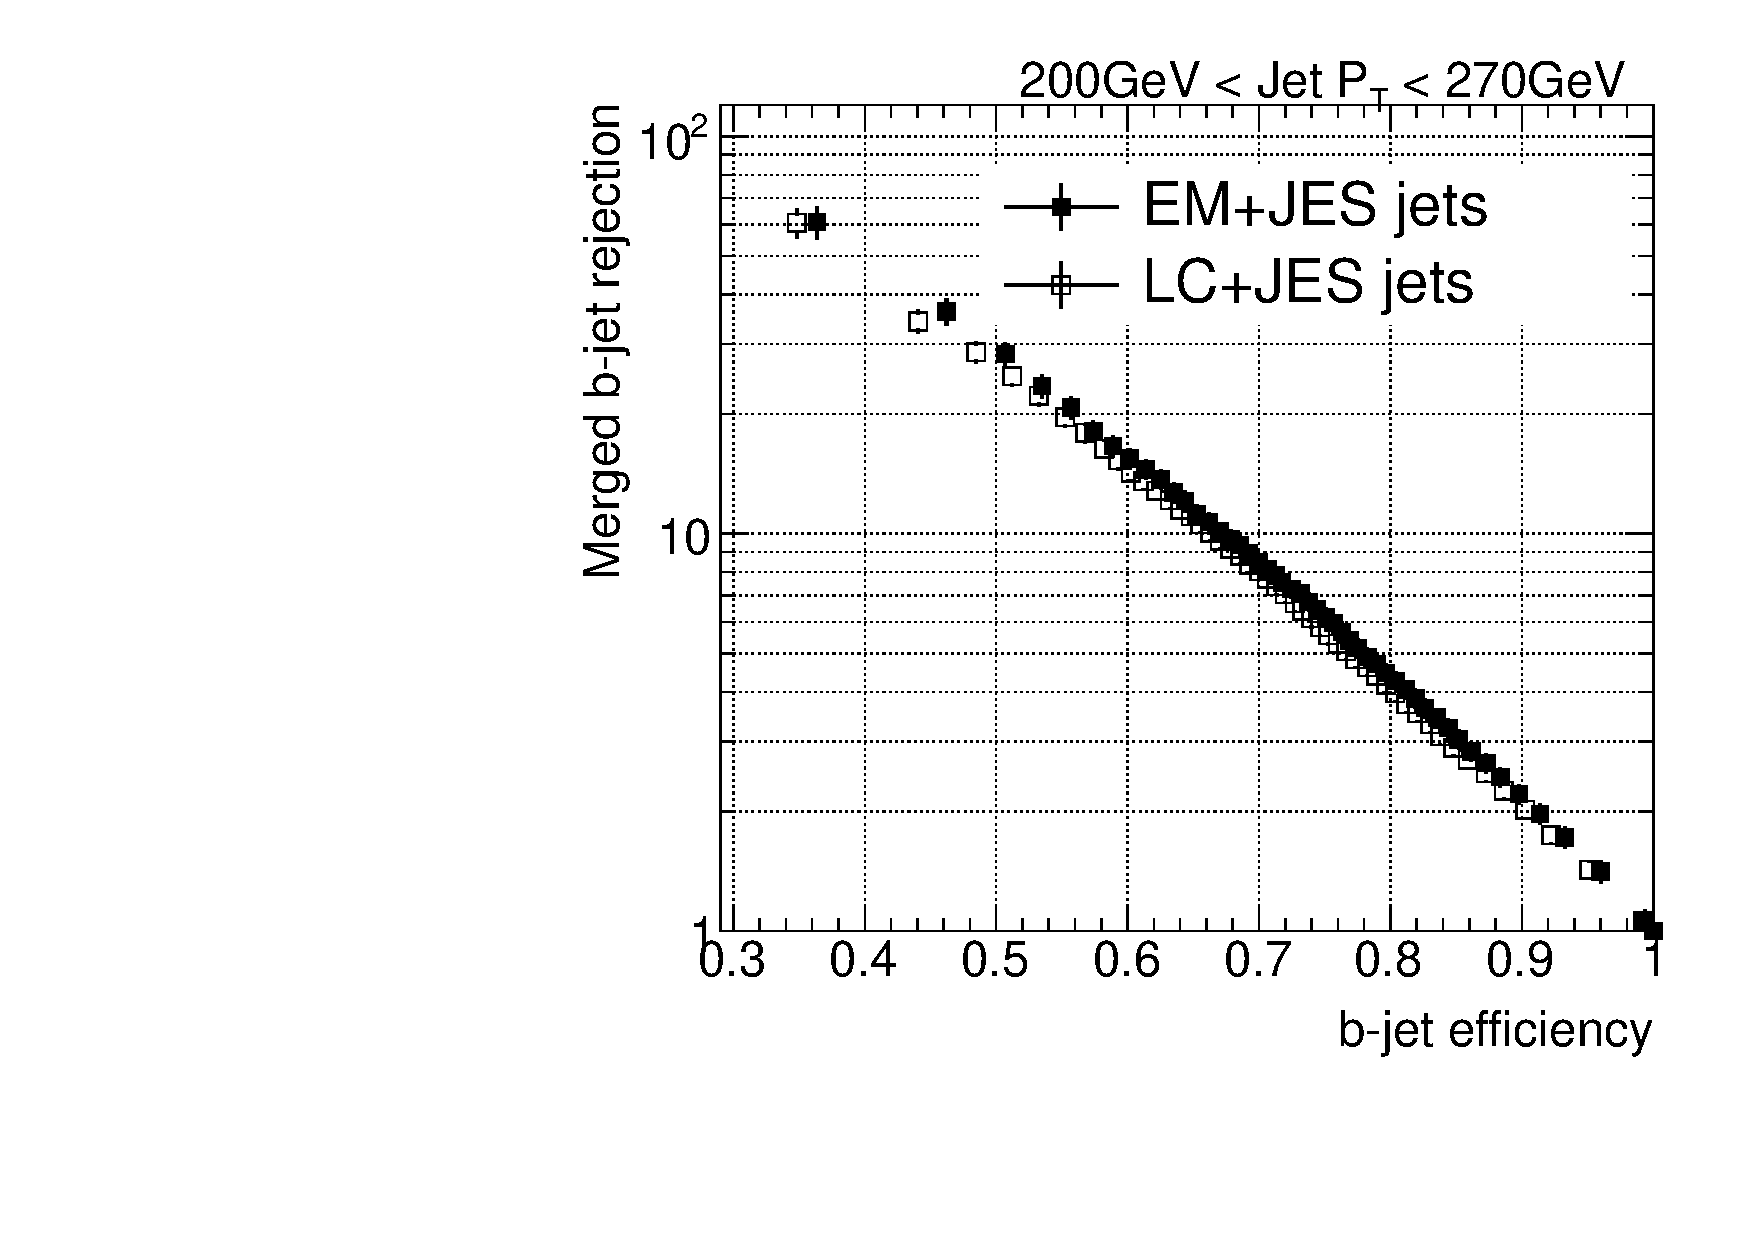
\includegraphics[width=0.49\textwidth]{FIGS/systematics/LlhoodKDE_ISO_LCcalibTest_rejvseff200.pdf}
\caption{Rejection of merged $b$-jets as a function of single $b$-jet efficiency for jets calibrated to the EM+JES (LC+JES) scale, between 80~GeV and 110~GeV and 200~GeV and 270~GeV.}
\label{fig:LCJES}
\end{figure}

%------------------------------------------------------------------------
%\section{Isolation studies}
%------------------------------------------------------------------------
%Although the tagger was derived with isolated jets it can also be applied to non-isolated jets. Studies were performed to evaluate the likelihood rejection in $b$-jets with close-by jet with $\pt$ between 7 GeV at electromagnetic scale and 90$\%$ of the $b$-jet $\pt$. The results can be seen in  Fig.~\ref{fig:testisolation}. The presence of close-by jets with a susbtancial fraction of the $b$-jet pt worsens the performance in more than 50$\%$ at very high $\pt$. 

%\begin{figure}[tp]
%\centering
%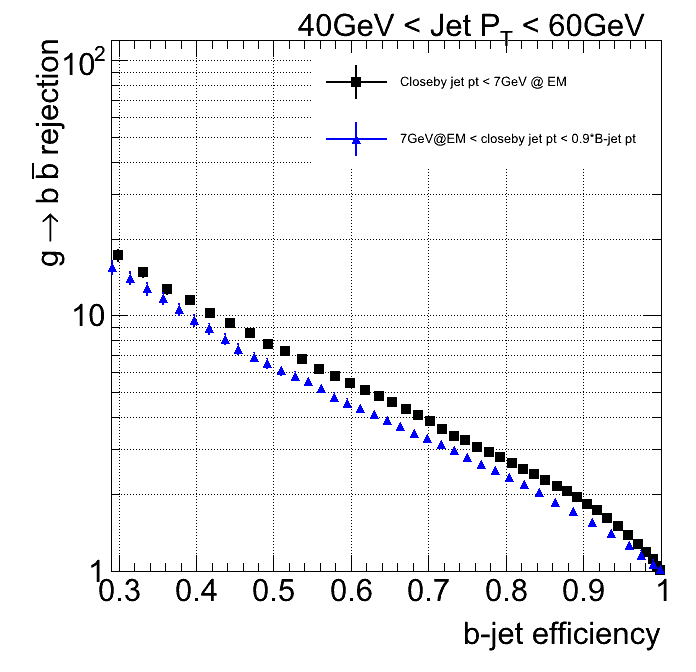
\includegraphics[width=0.4\textwidth]{FIGS/systematics/DiffIsolationCutsKDE_RejvsEff40.png}
%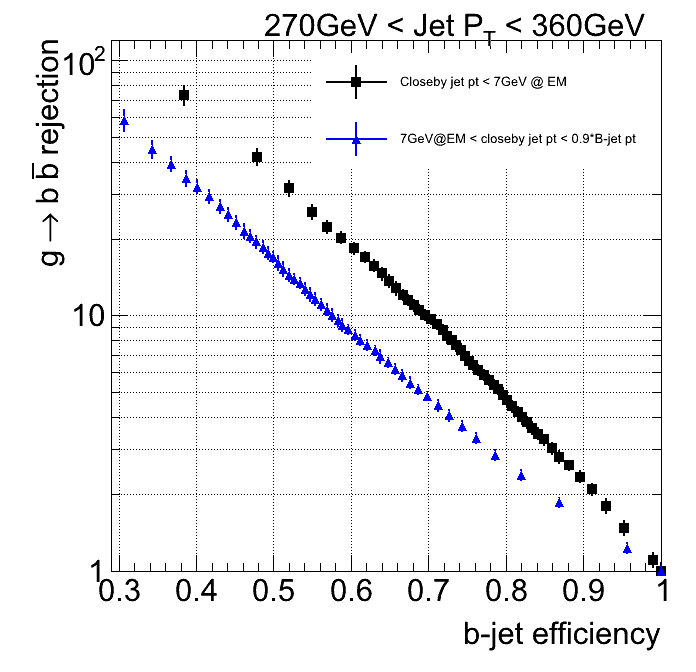
\includegraphics[width=0.4\textwidth]{FIGS/systematics/DiffIsolationCutsKDE_RejvsEff270.png}
%\caption{Rejection of merged $b$-jets as a function of single $b$-jet efficiency for two different isolation cuts.}
%\label{fig:testisolation}
%\end{figure}


%------------------------------------------------------------------------
\section{Other Monte Carlo generators}\label{sec:otherMC}
%------------------------------------------------------------------------
%{\em Uncertainties due to the event modelling in the Monte Carlo generators}

The development, training and performance determination of the tagger has been done using Monte Carlo events generated with the {\sc pythia} event simulator, interfaced to the {\sc geant4} based simulation of the ATLAS detector. An immediate question is what the performance would be if studied with a different simulation. In this section we investigate this question for the {\sc pythia} Perugia tune  and the {\sc herwig++} event generators (Section~\ref{sec:MCtools}).

Fig.~\ref{fig:performanceotherMC} shows a comparison of the likelihood rejection, at the 50\% efficiency working point,  between nominal {\sc pythia} and the alternative simulations % for four selected $\pt$ bins covering the full kinematic range. 
as a function of the jet $\pt$ . The larger errors are due to the reduced statistics available, which are even lower for the Perugia case than for {\sc herwig}.



%In order to account for the dependence on different generator models and tunes the likelihood performance was tested using other Monte Carlo simulations. Results with nominal Pythia were compared to the performance derived with dijet samples generated with Herwig++ and with the Perugia tune of Pythia. The comparison can be seen in Fig.~\ref{fig:performanceotherMC}. 

The performance in {\sc herwig} shows a systematic trend, with agreement at low $\pt$ and increasingly poorer performances compared to {\sc pythia} as $\pt$ grows. For the Perugia tune, on the other hand, there is no definite behavior, with the performance fluctuating above or below the nominal simulation for different $\pt$ bins consistently with the statistical uncertainties.

The reason for the systematic difference observed between the performances of {\sc pythia} and {\sc herwig} can be traced to the extent with which jets are accurately modelled. Fig.~\ref{fig:herwigdatamc} compares the measured jet track multiplicity distributions in $b$-tagged jets and the prediction from both simulations, for low and high $\pt$ jets. It is observed that indeed {\sc herwig++} does not correctly reproduce the data, particularly at high $\pt$. The level of agreement is found to be better for track-jet width and the $\Delta R$ between the axes of the two $k_t$ subjets in the jet, the two other variables used for discrimination.


The more accurate description of $b$-jet substructure in {\sc pythia} than in {\sc herwig++} had been previously observed in ATLAS. It is due to the inclusion in {\sc pythia} of a detailed study of the $b$-quark fragmentation function based on LEP and SLD data~\cite{JESUncertainty}.




%the comparion between jet distribution in experimental data and  Herwig++ Monte Carlo events was performed for $b$-tagged jets. The results for the jet track-multiplicity can be seen in Fig.~\ref{fig:herwigdatamc}. We find that Herwig++ does not reproduce data jet distributions correctly at medium and high $\pt$.



\begin{figure}[tp]
\centering
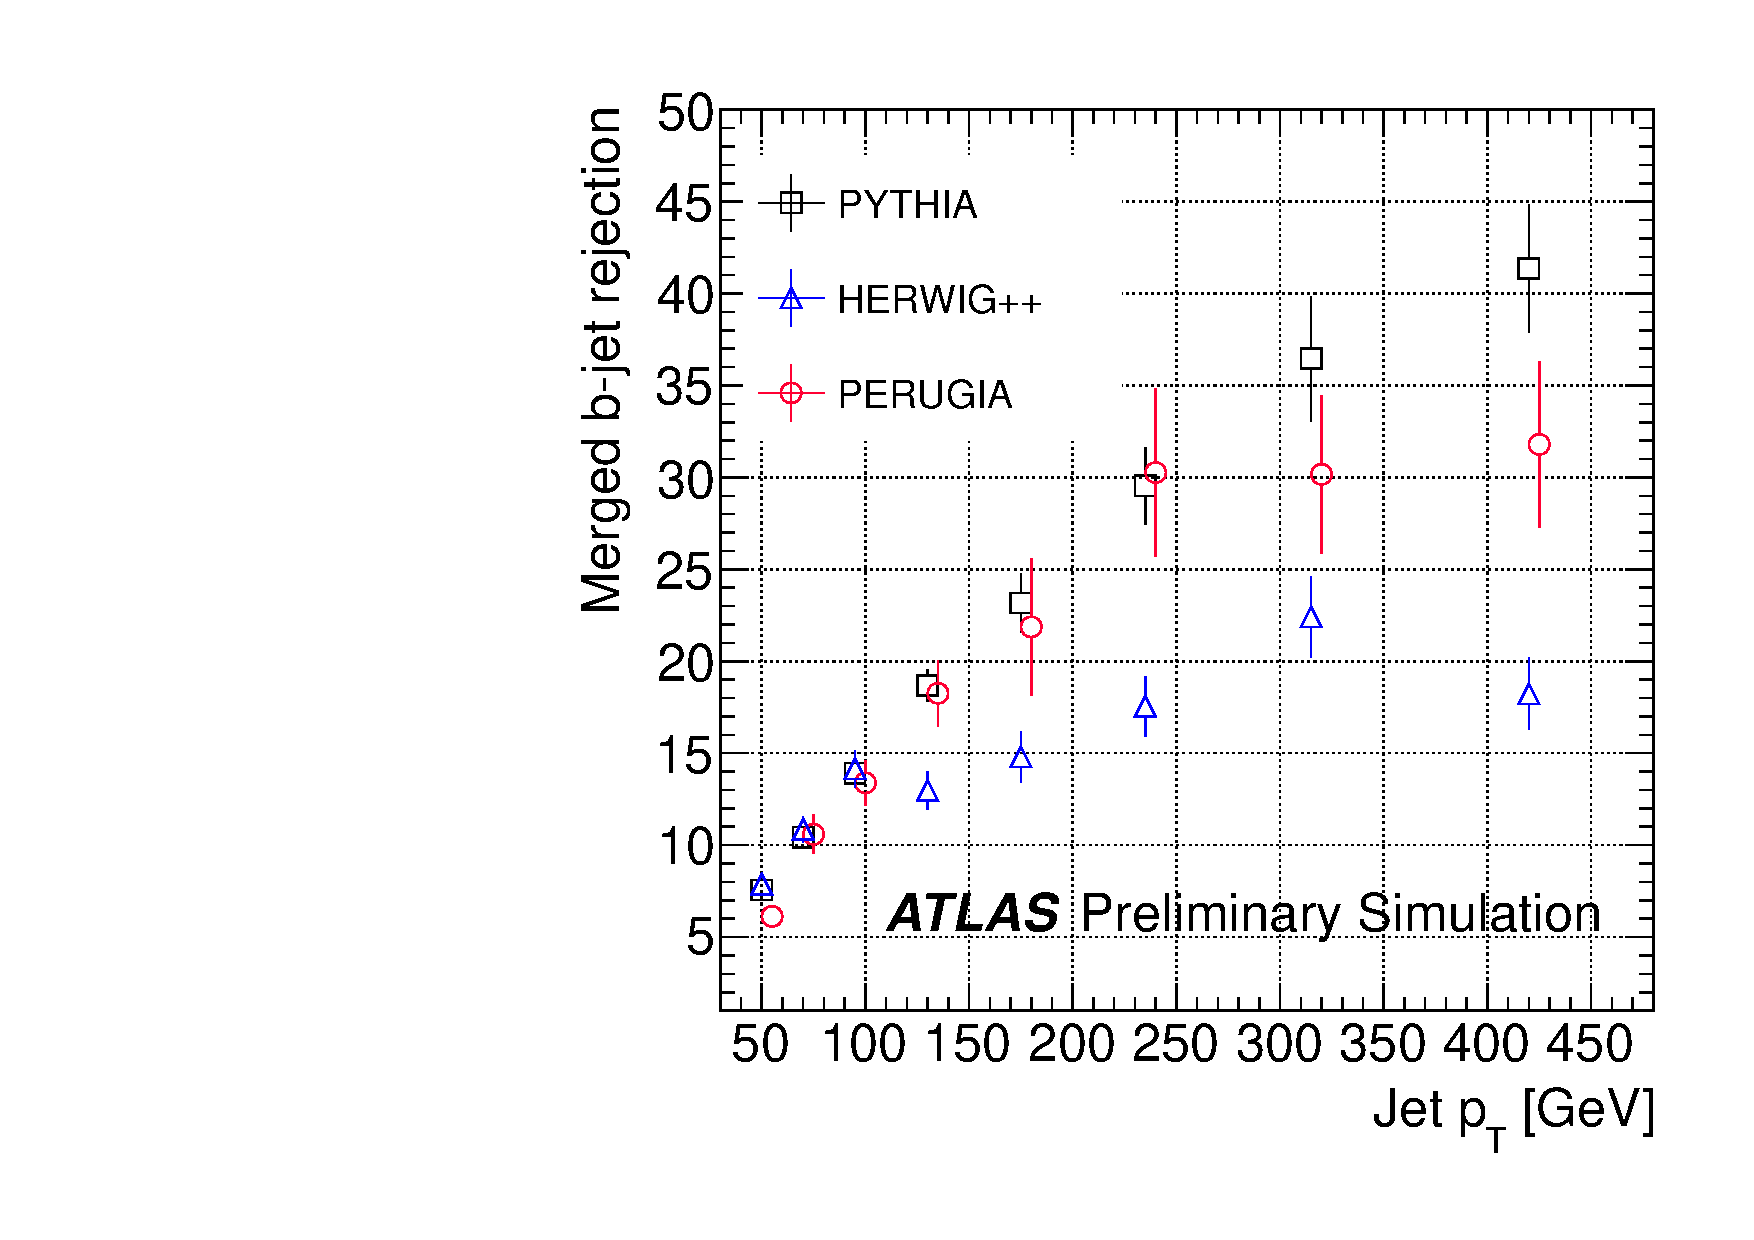
\includegraphics[width=0.7\textwidth]{gbbRejection_vs_PT_3MonteCarlos_50Eff_shift5.pdf}
%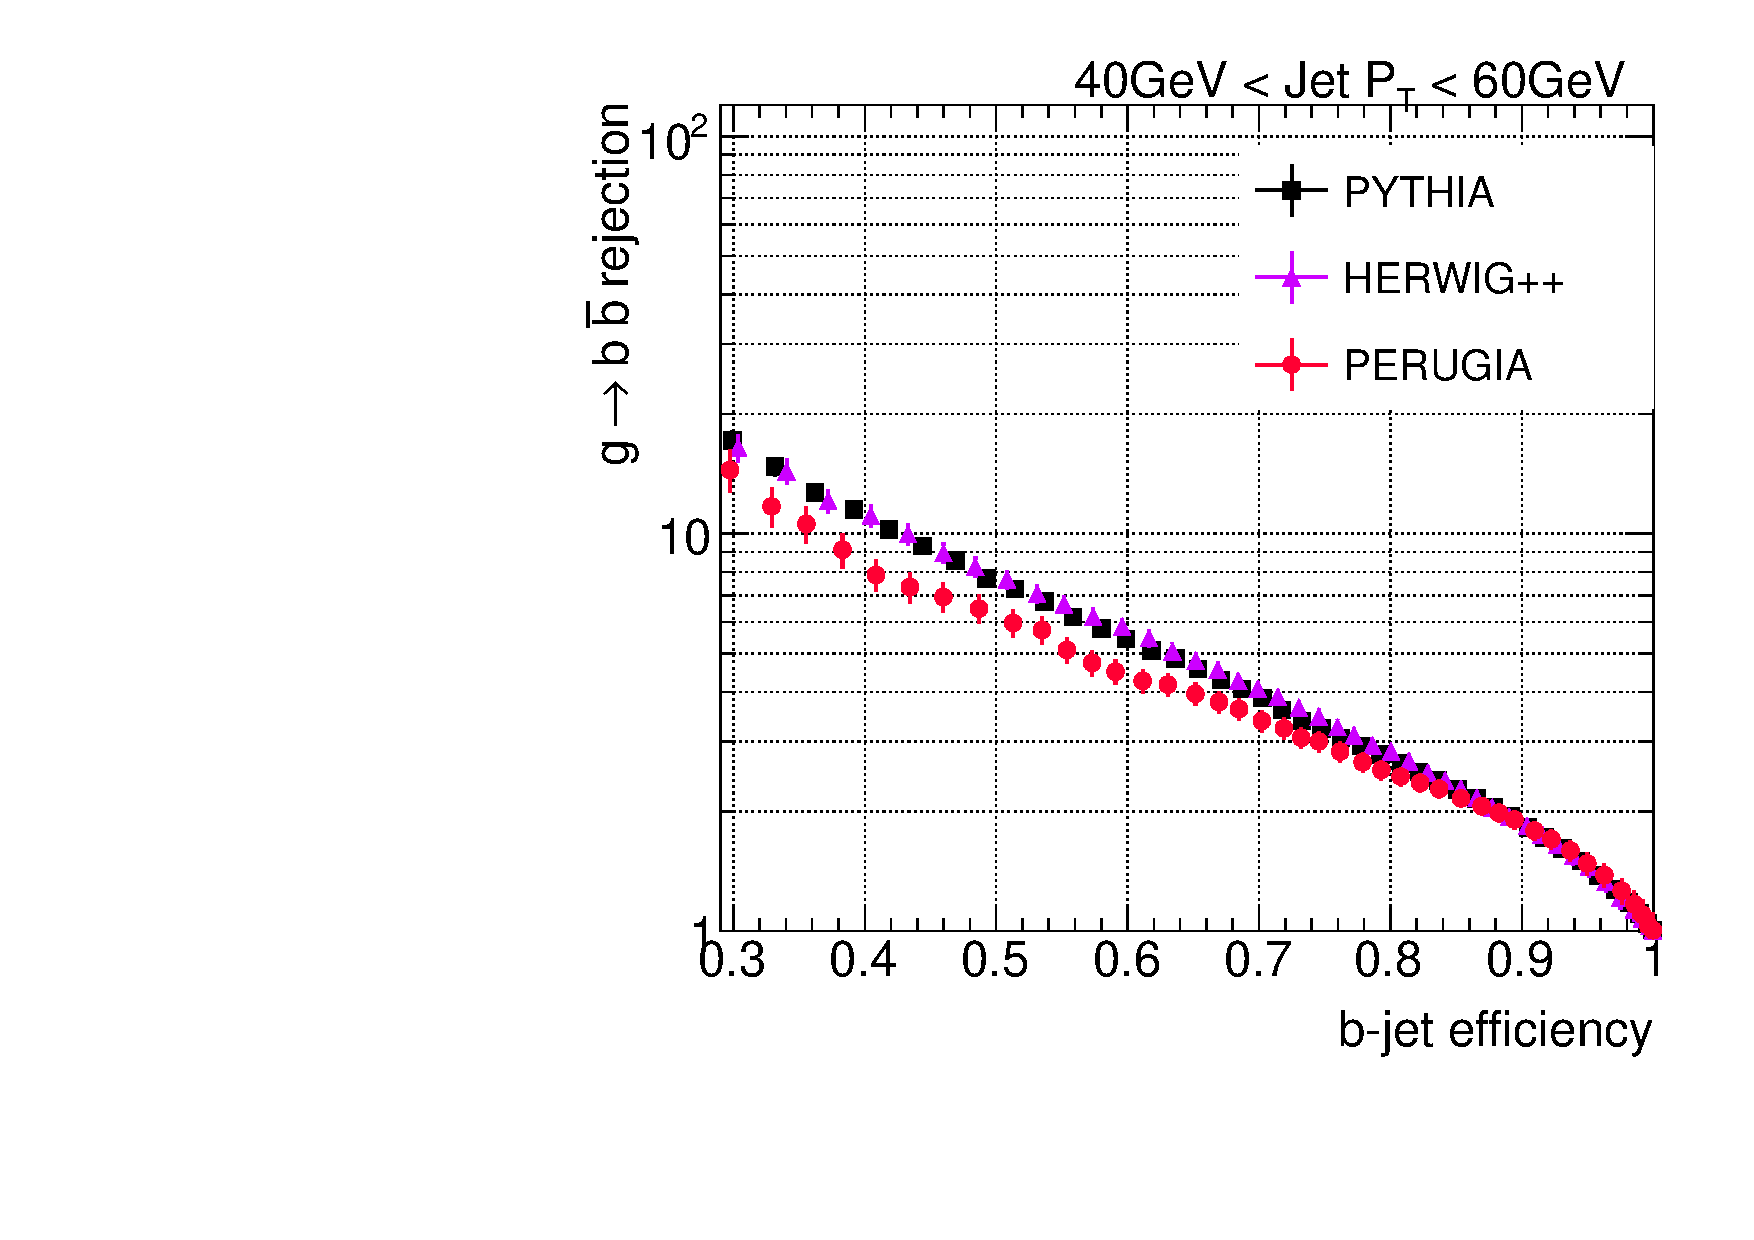
\includegraphics[width=0.49\textwidth]{FIGS/systematics/newInterpLlhoodKDE_ISO_DiffMCGen_rejvseff040.pdf}
%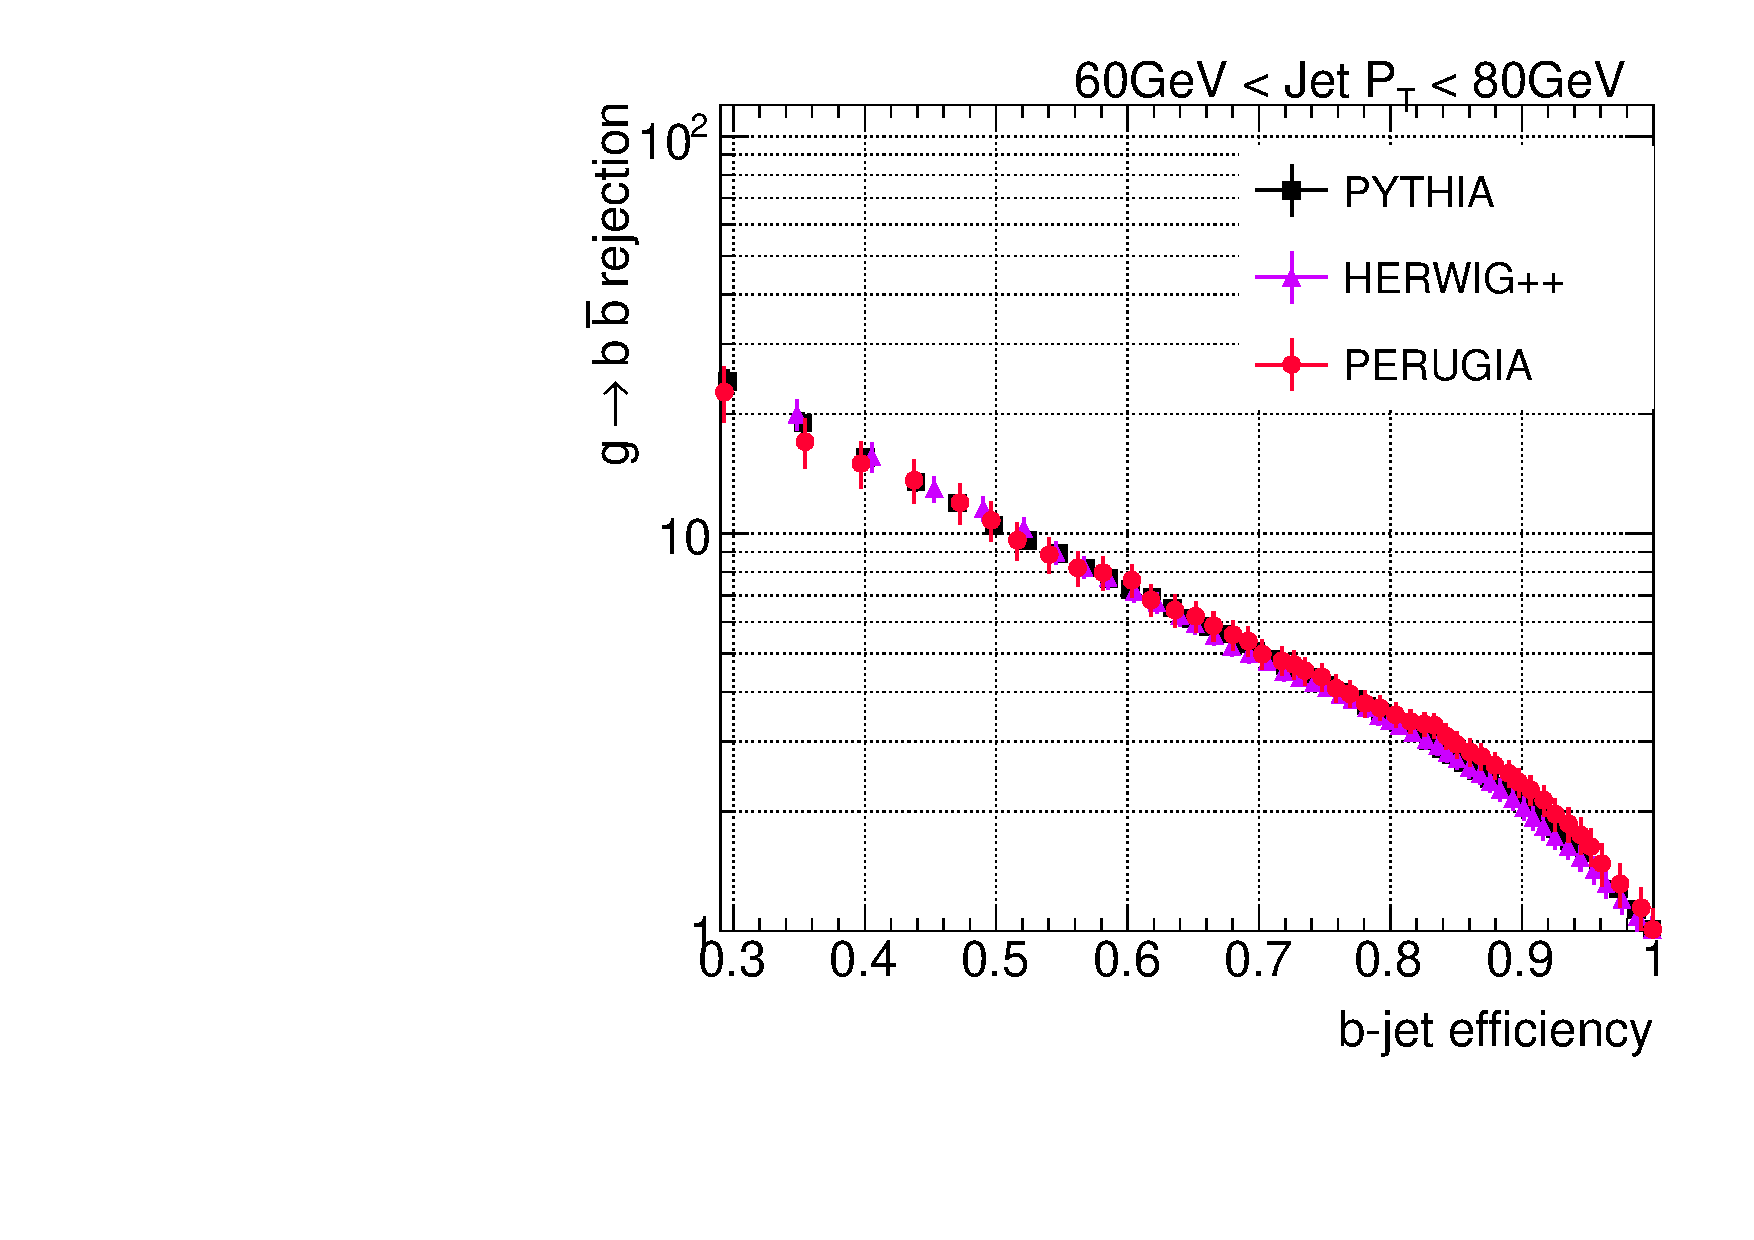
\includegraphics[width=0.49\textwidth]{FIGS/systematics/newInterpLlhoodKDE_ISO_DiffMCGen_rejvseff060.pdf}
%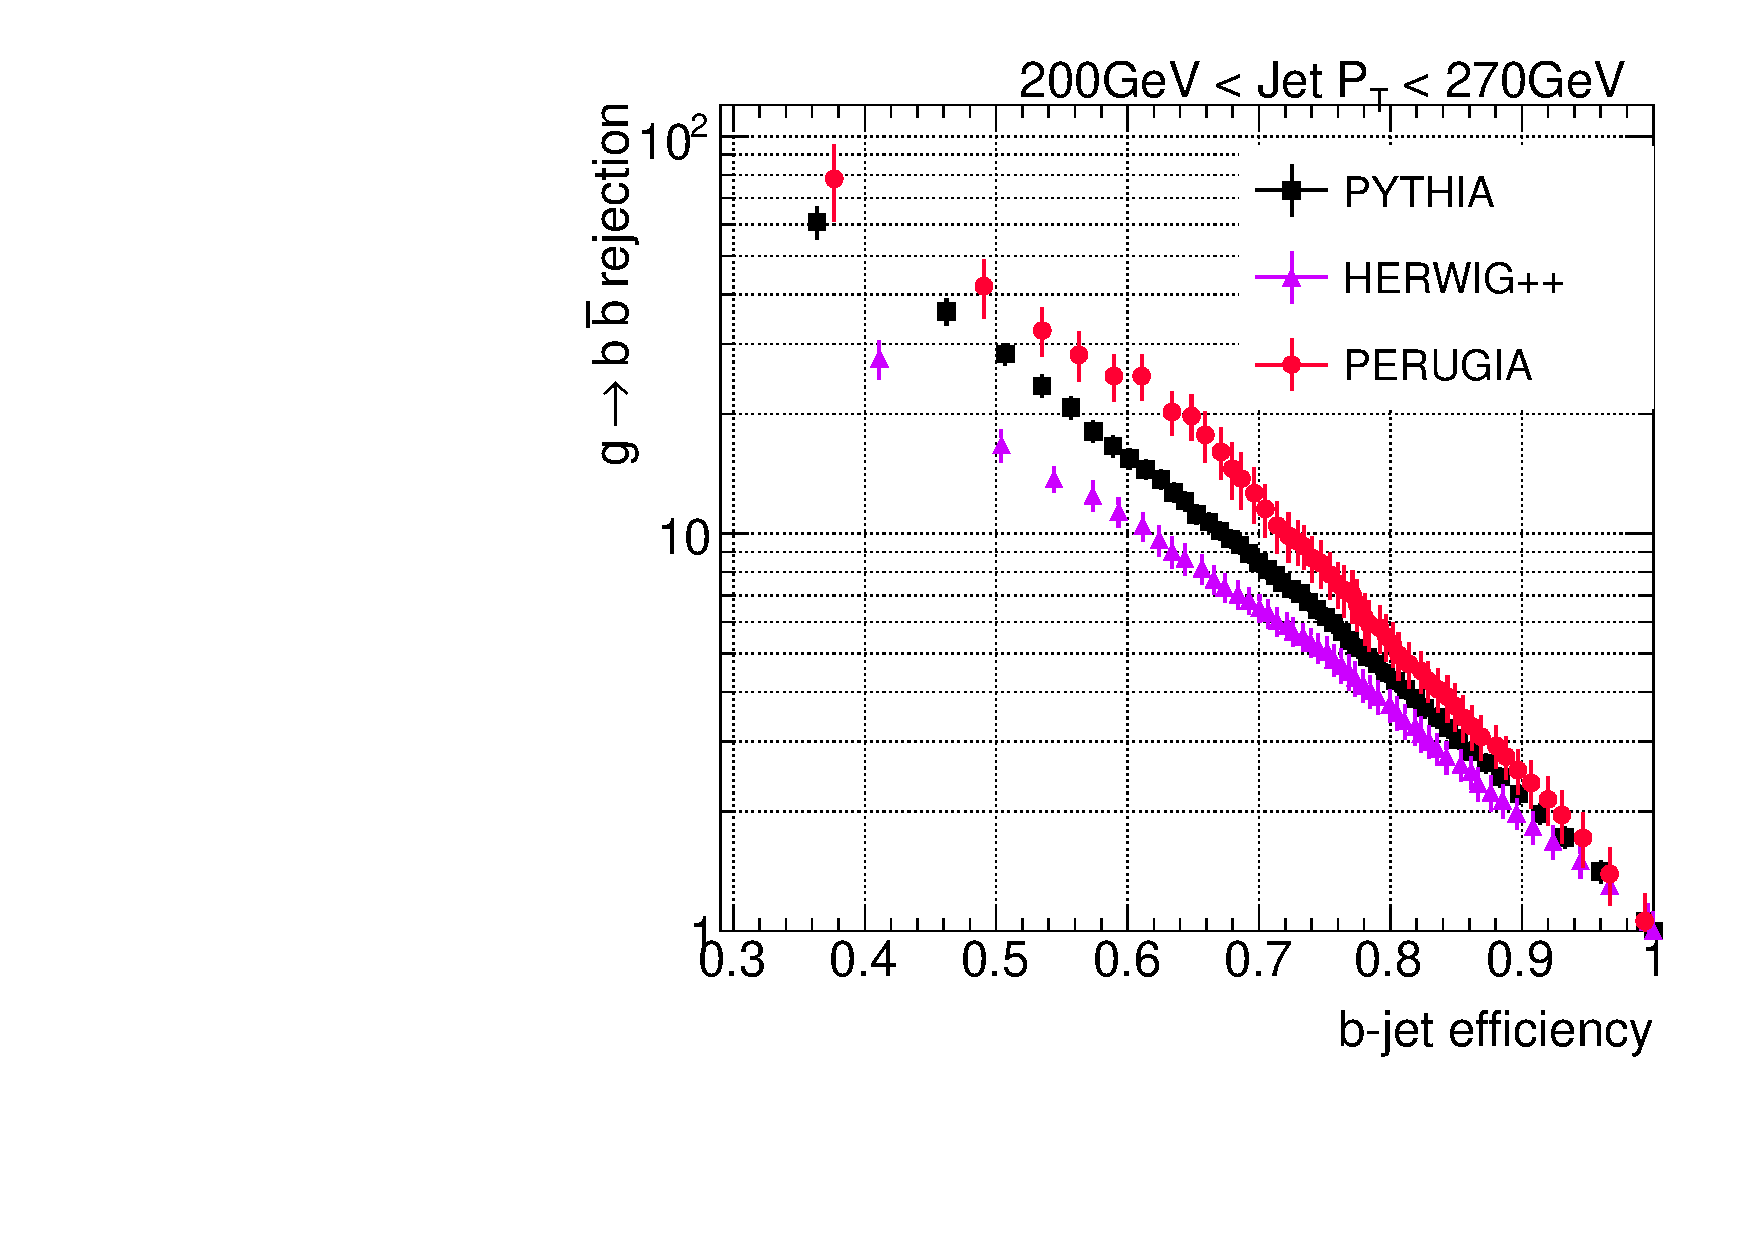
\includegraphics[width=0.49\textwidth]{FIGS/systematics/newInterpLlhoodKDE_ISO_DiffMCGen_rejvseff200.pdf}
%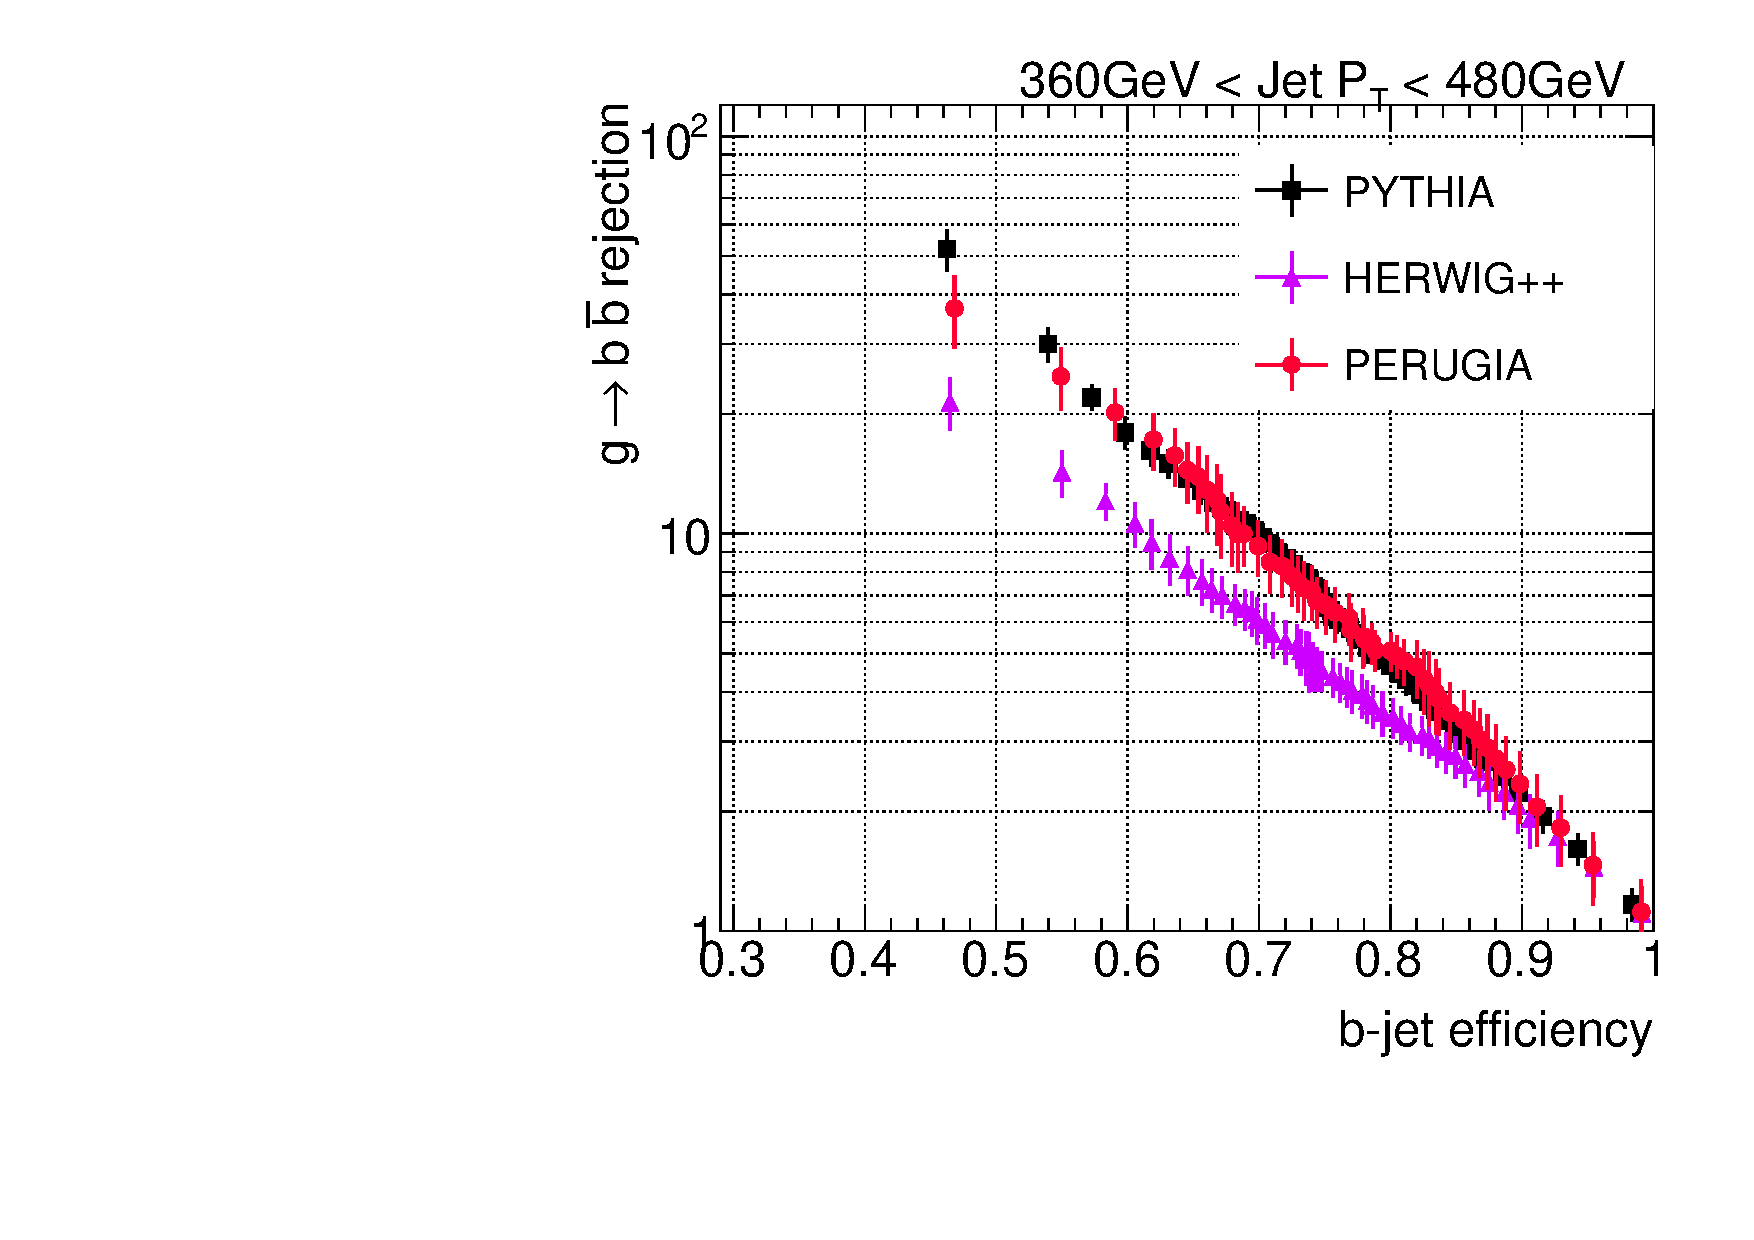
\includegraphics[width=0.49\textwidth]{FIGS/systematics/newInterpLlhoodKDE_ISO_DiffMCGen_rejvseff360.pdf}
\caption{Rejection of merged $b$-jets as a function of jet $\pt$ for different Monte Carlo generators, at the 50\% efficiency working point. The Perugia points are shifted by $+$5~GeV for display purposes.}
\label{fig:performanceotherMC}
\end{figure}

\begin{figure}[tp]
\centering
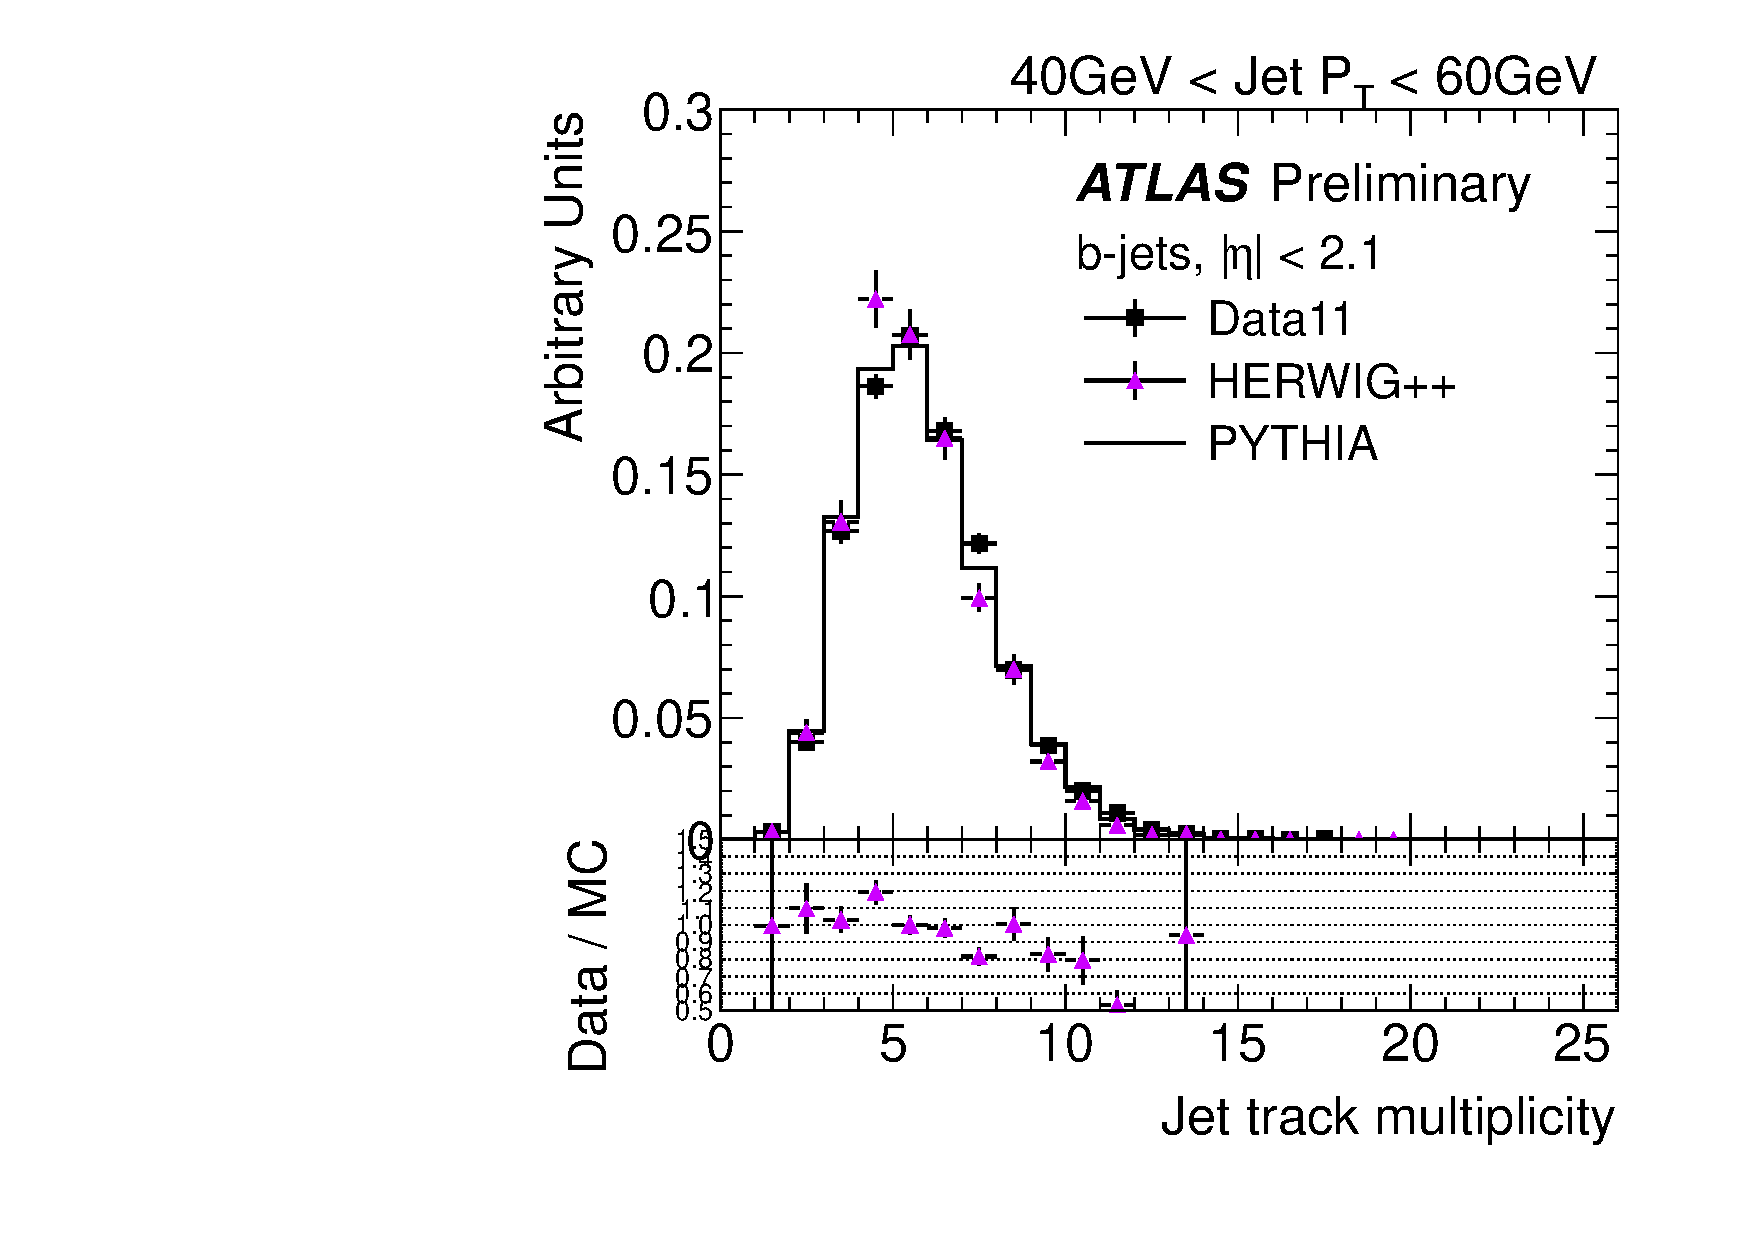
\includegraphics[width=0.49\textwidth]{FIGS/systematics/DataVarNtrkPT040.pdf}
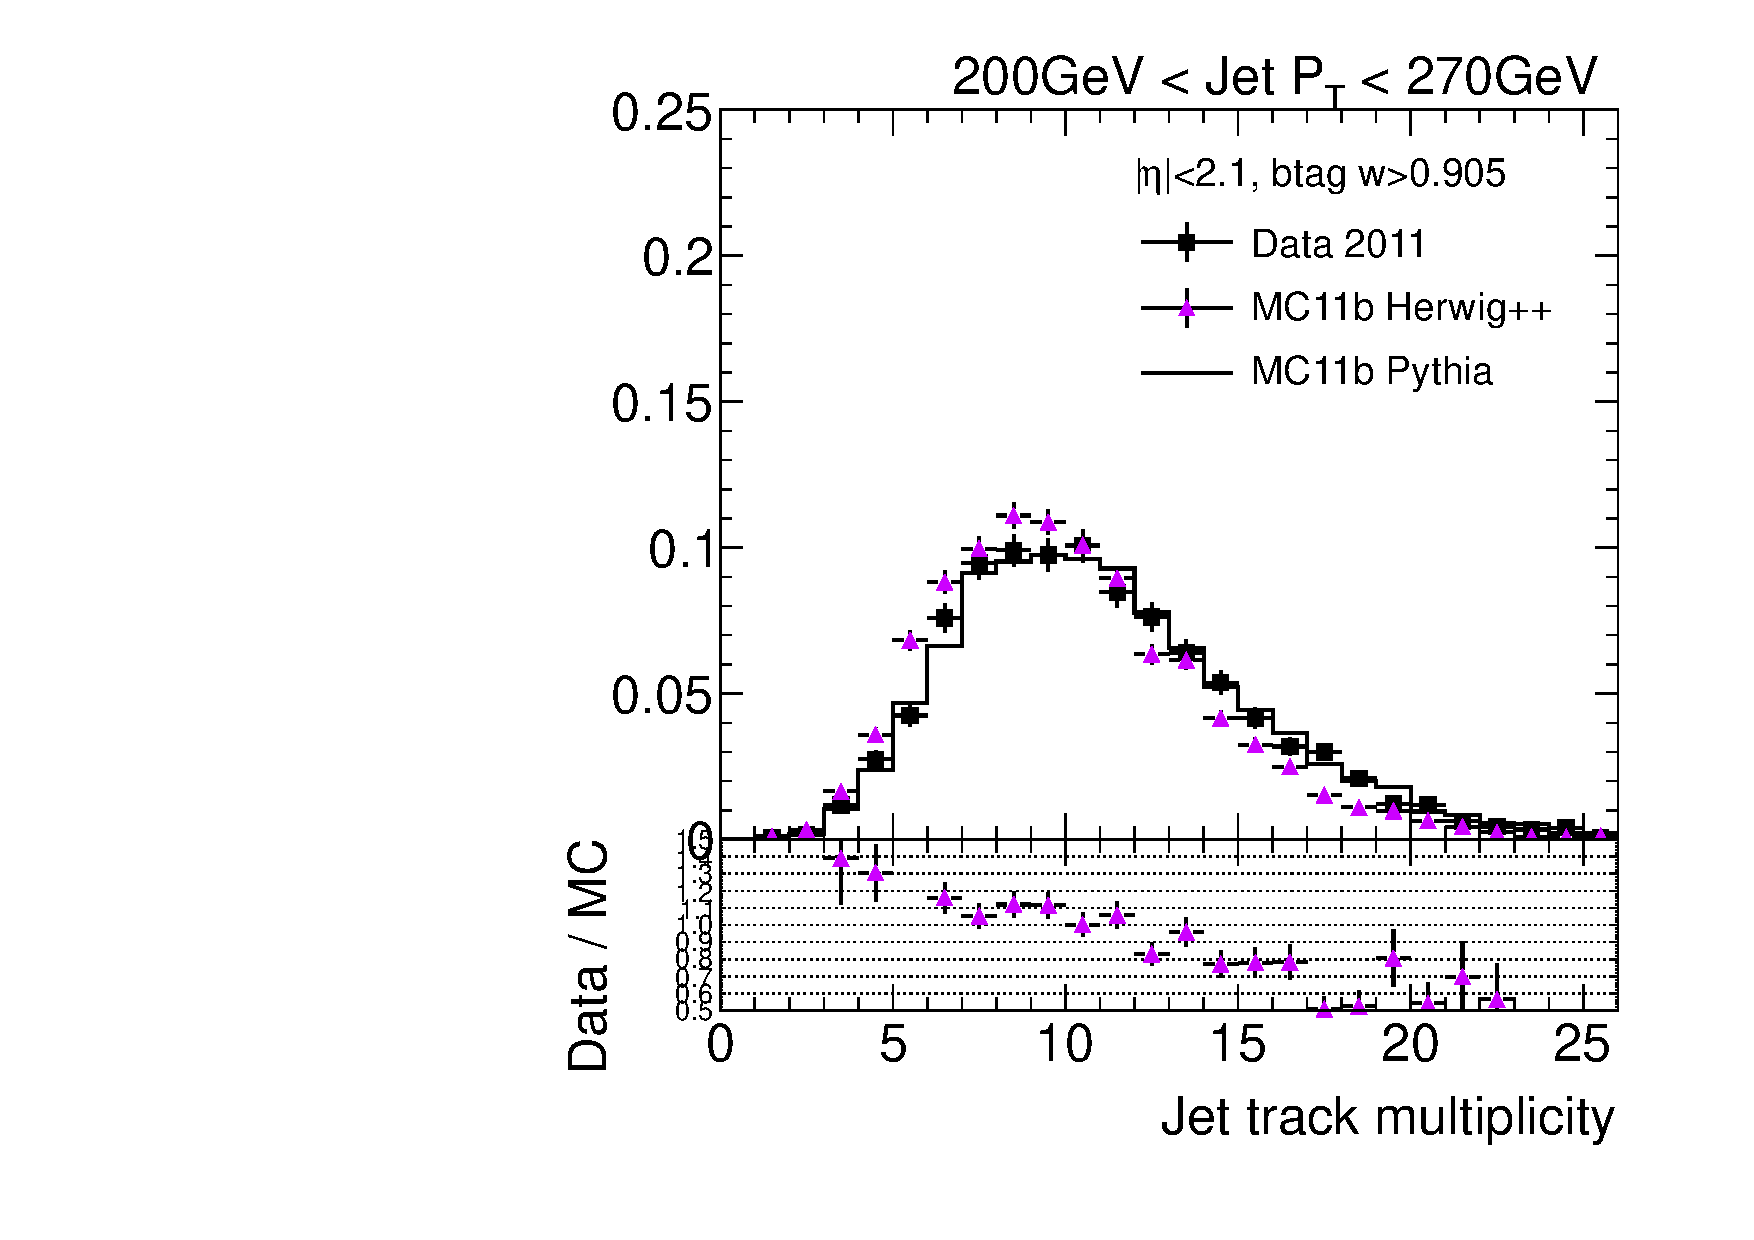
\includegraphics[width=0.49\textwidth]{FIGS/systematics/DataVarNtrkPT200.pdf}
\caption{Distribution of the jet track multiplicity in 2 different jet $\pt$ bins, for experimental data  collected during 2011 (solid black points) and {\sc herwig}++ events (solid violet triangules). The ratio data over {\sc herwig}++ simulation is shown at the bottom of the plot. {\sc pythia} distribution is also shown for reference.}
\label{fig:herwigdatamc}
\end{figure}



%------------------------------------------------------------------------
%\section{Validation of the MVA output in data}\label{sec:MVAvalidation}
%------------------------------------------------------------------------

%In Section~\ref{sec:gbbValidation} the validation of the tracking variables in data from 2011 runs was presented,  showing an excellent agreement between experimental data and the Monte Carlo simulation. In particular, the agreement obtained for the track multiplicity, the track-jet width and the $\Delta R$ between $k_t$ axes - the three input variables -  is shown in Fig.~\ref{fig:datamcmva}. 

%The likelihood presented in this chapter is an observable built out of the three selected variables and, for this reason, a similar level of agreement is expected for the output distributions in bins of the jet transverse momentum.  Figures~\ref{fig:datamcmva} shows the distribution of the likelihood output for different bins of jet $\pt$. The agreement is excellent.


%\begin{figure}[tp]
%\centering
%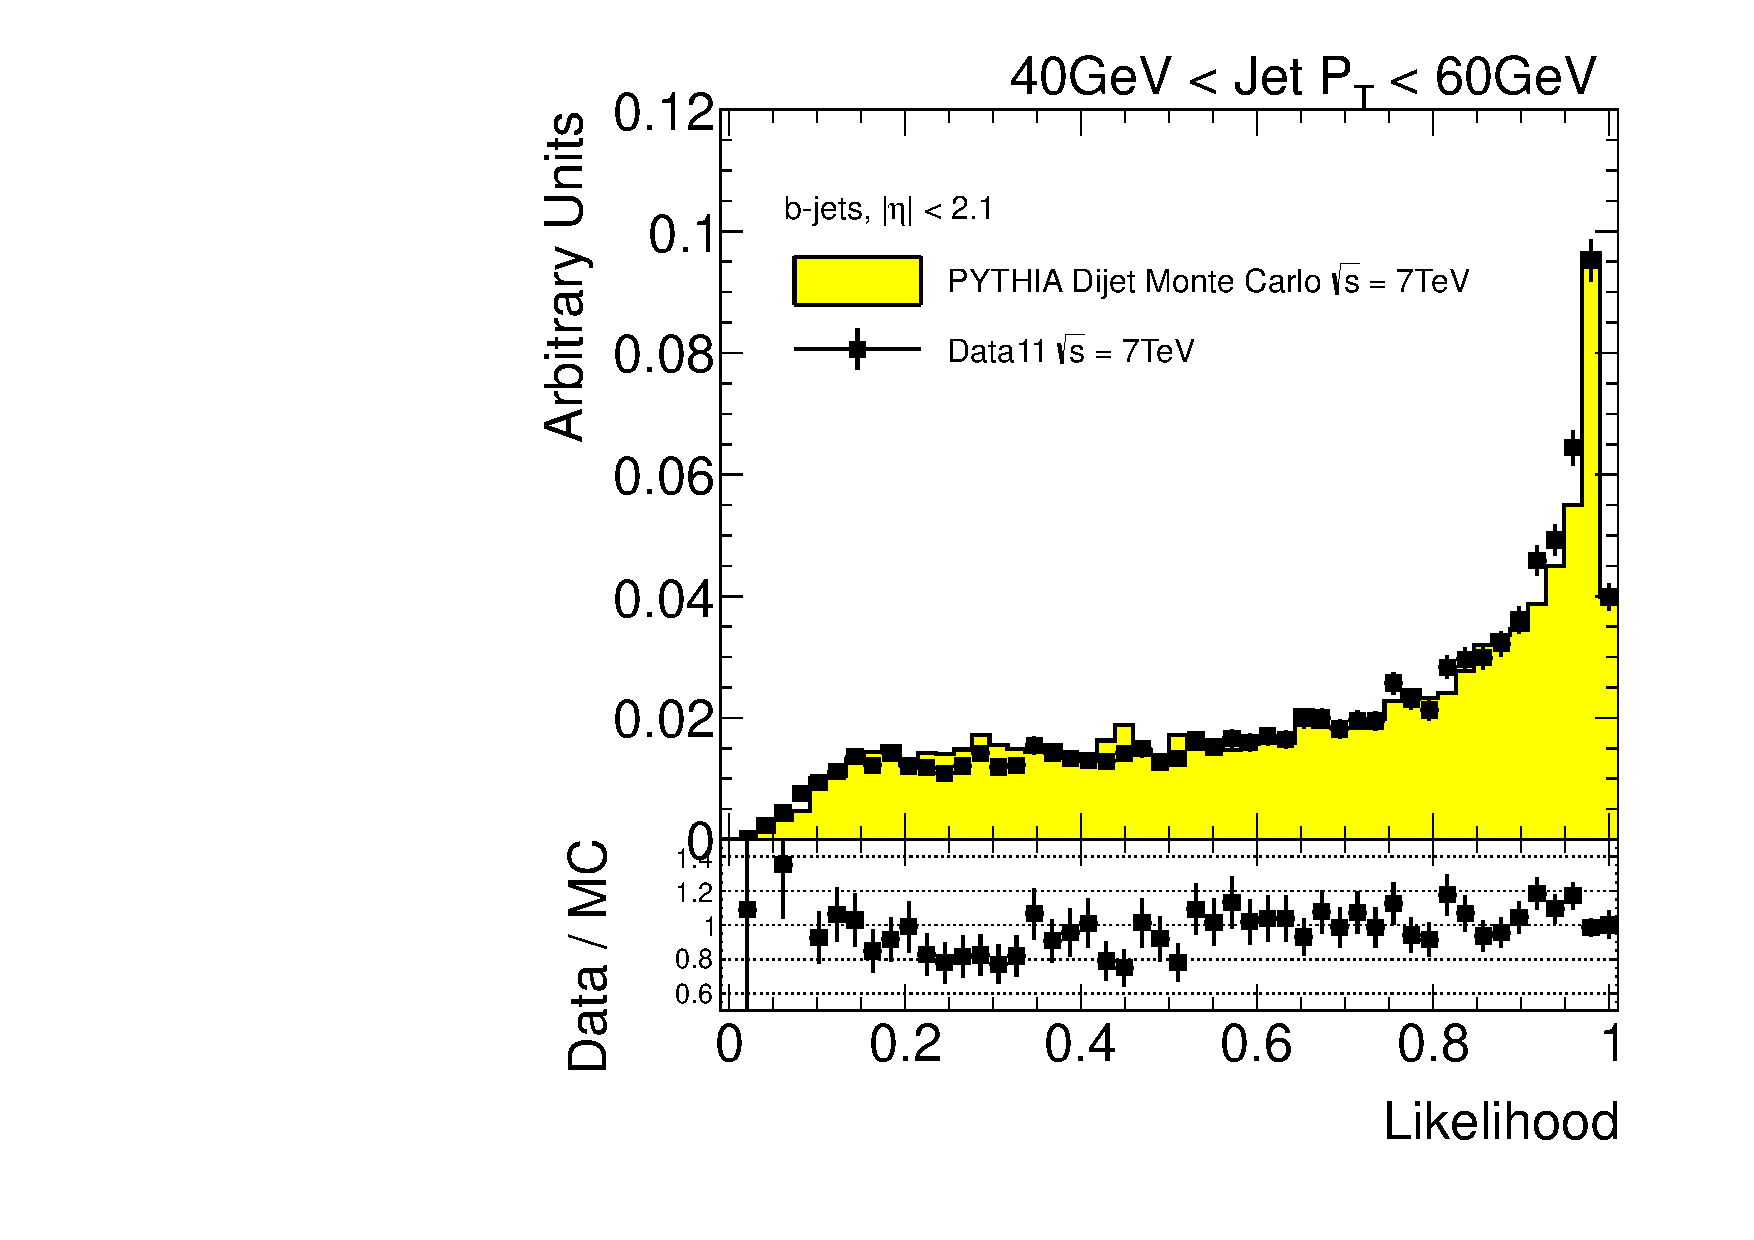
\includegraphics[width=0.49\textwidth]{FIGS/dataMC/likelihood/FullMVAoutput_PT040.pdf}
%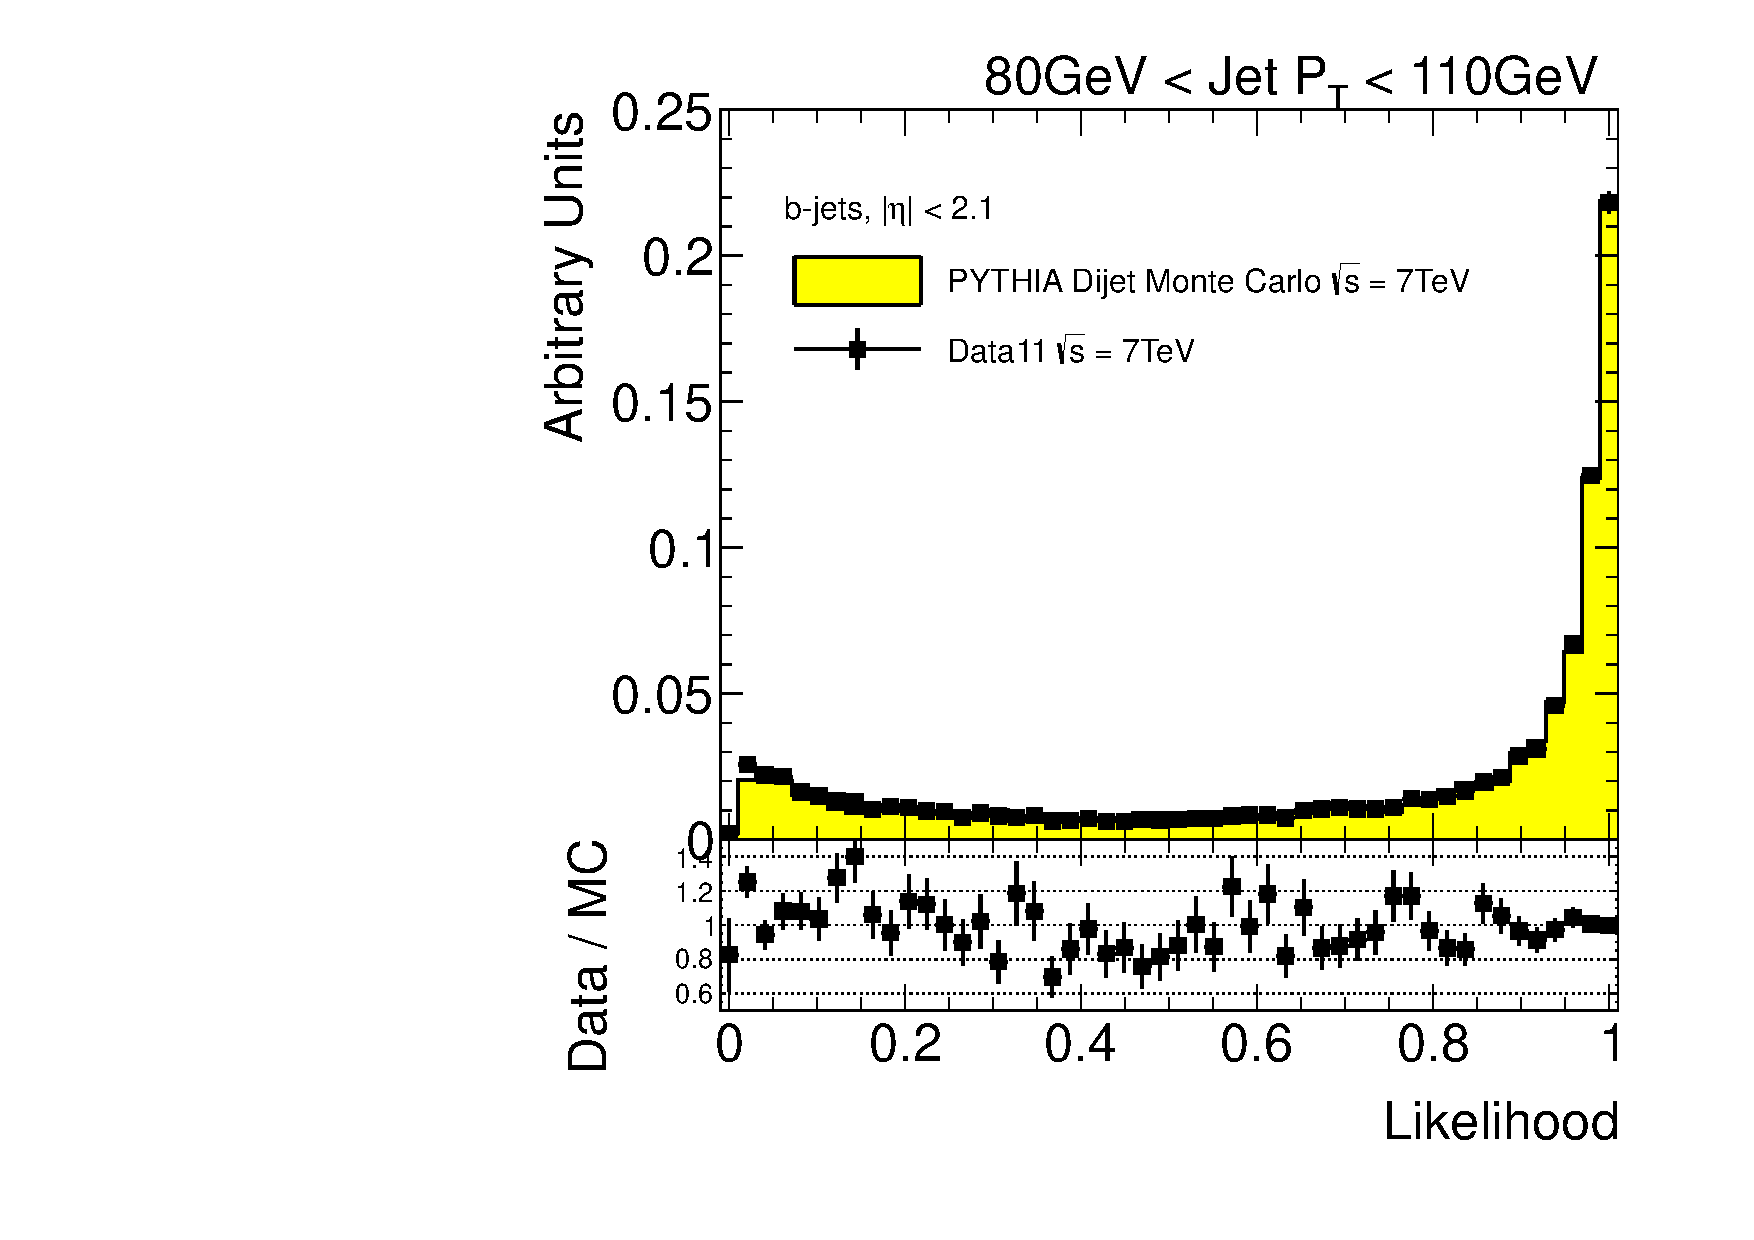
\includegraphics[width=0.49\textwidth]{FIGS/dataMC/likelihood/FullMVAoutput_PT080.pdf}
%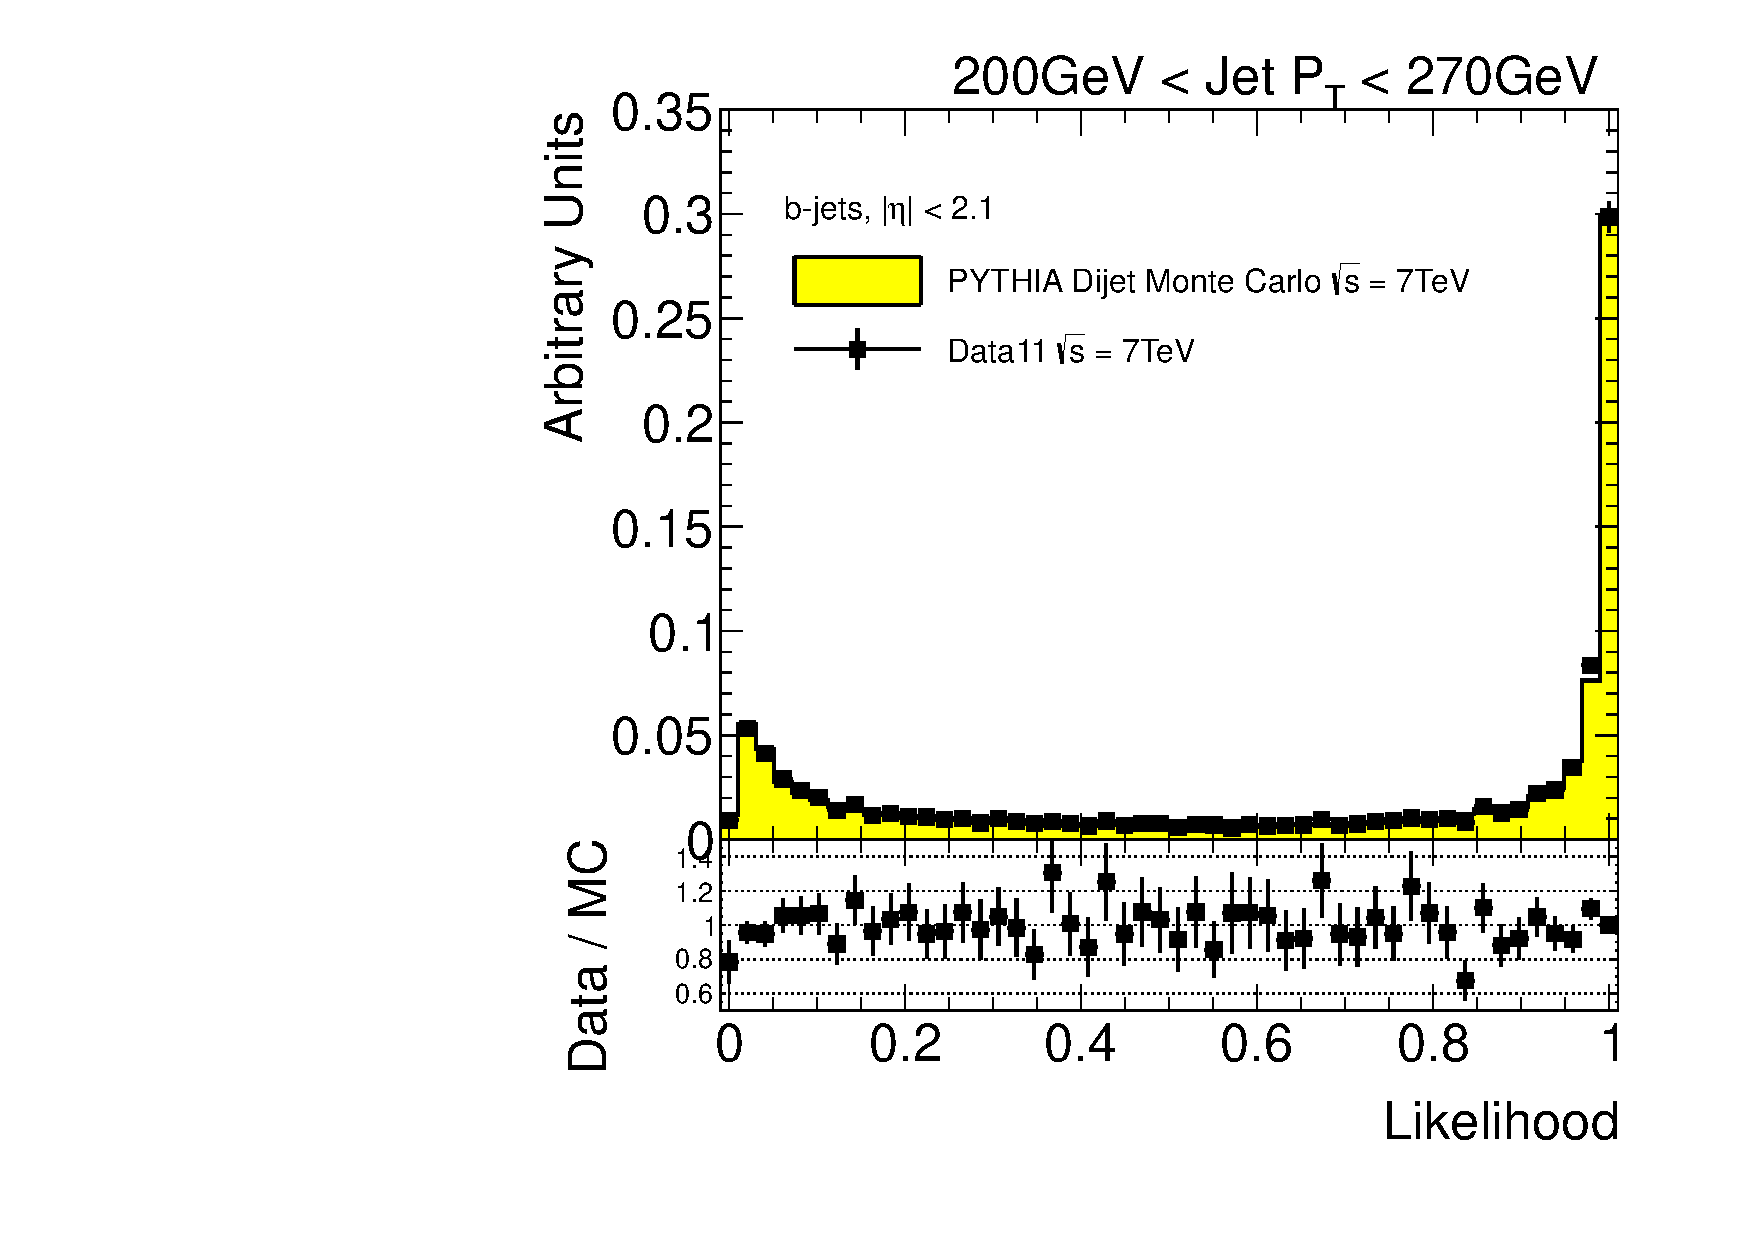
\includegraphics[width=0.49\textwidth]{FIGS/dataMC/likelihood/FullMVAoutput_PT200.pdf}
%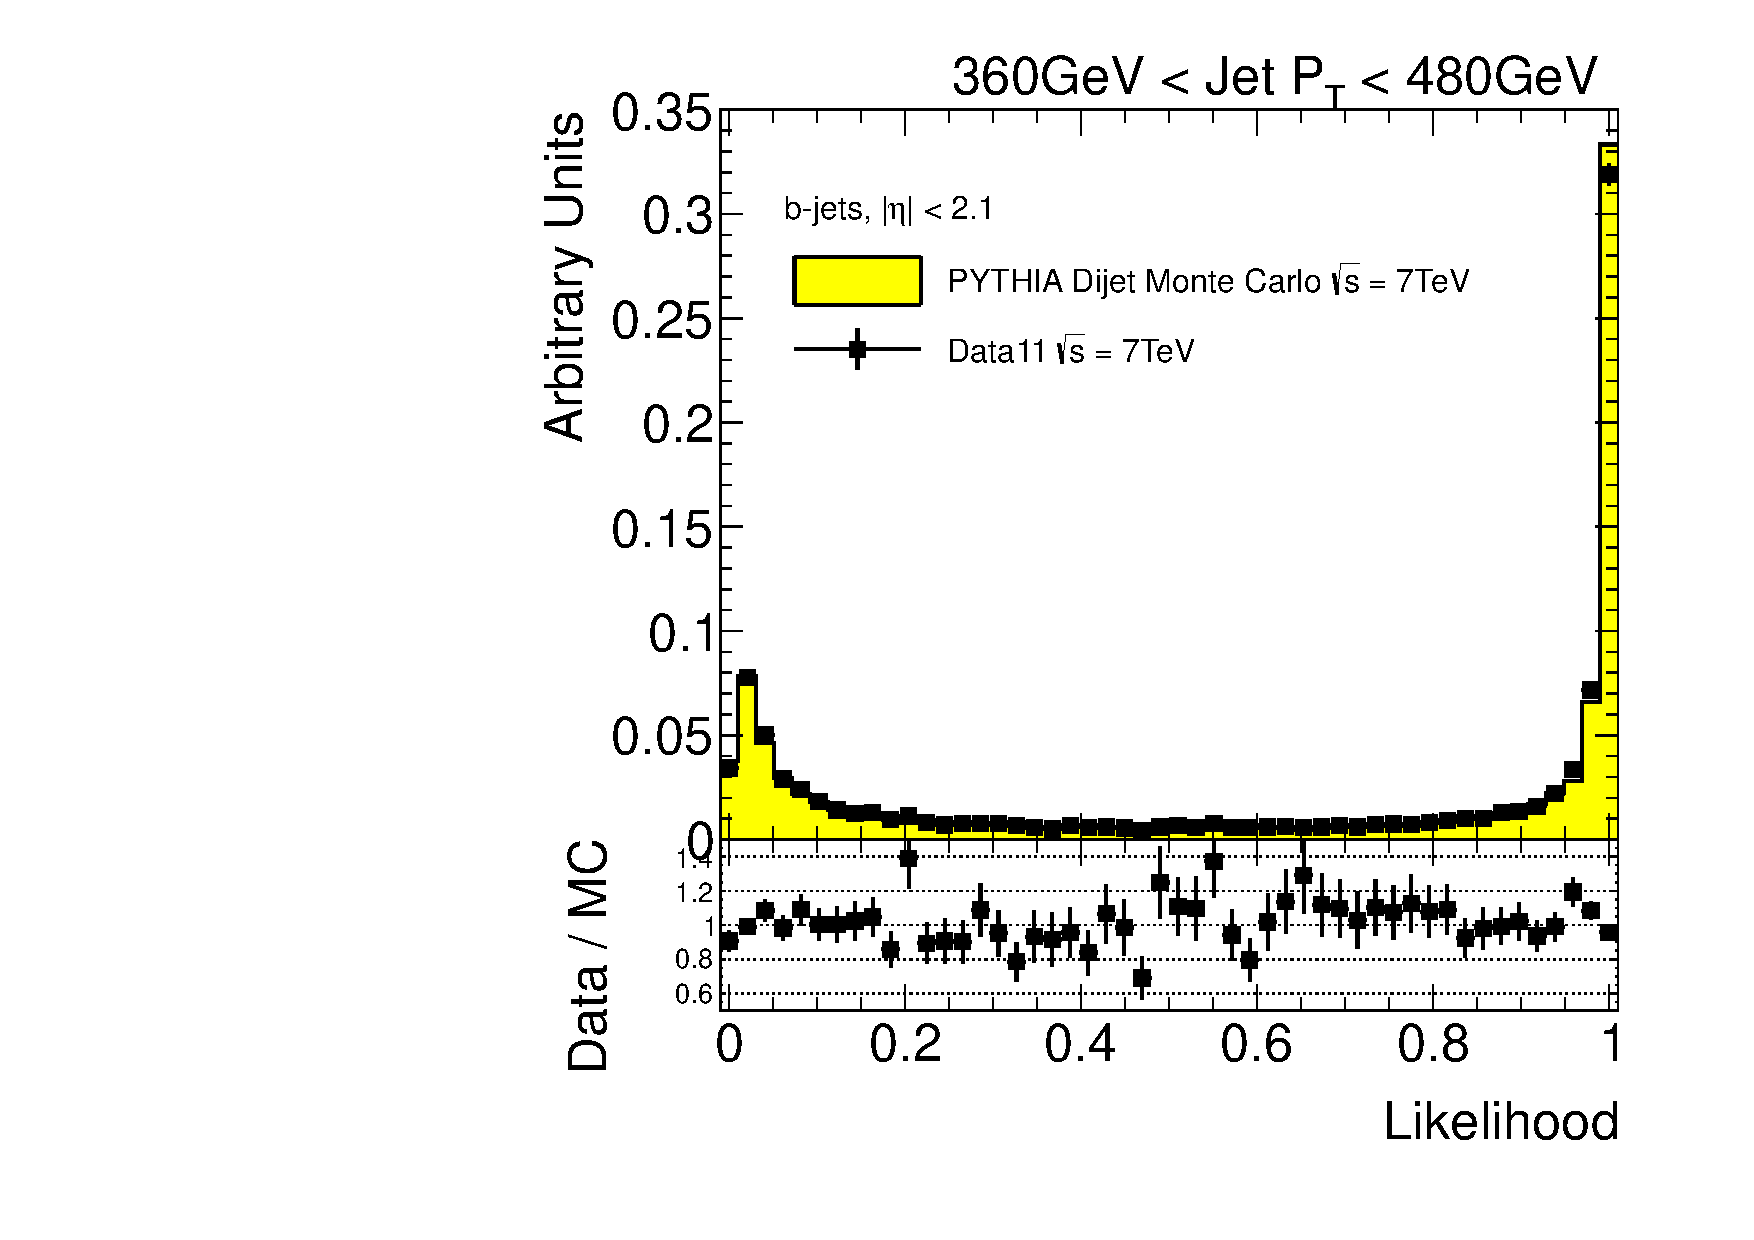
\includegraphics[width=0.49\textwidth]{FIGS/dataMC/likelihood/FullMVAoutput_PT360.pdf}  
%\caption{ Distribution of likelihood output in different jet $\pt$ bins, for experimental data  collected by ATLAS during 2011 (solid black points), and simulated data (filled histograms). The ratio data over simulation is shown at the bottom of each plot.}
%\label{fig:datamcmva}
%\end{figure}
